%%%%%%%%%%%%%%%%%%%%%%%%%%%%%%%%%%%%%%%%%%%%%%%%%%%%
%
% Versione: 0.1
%
%%%%%%%%%%%%%%%%%%%%%%%%%%%%%%%%%%%%%%%%%%%%%%%%%%%%

\documentclass{book}

\usepackage[a4paper, total={16cm, 25cm}]{geometry}
\usepackage[utf8]{inputenc}
\usepackage[sfdefault]{cabin}
\usepackage[italian]{babel}
\usepackage[parfill]{parskip}

\usepackage{fancyhdr} 
\fancyhf{}
\cfoot{\thepage}
\pagestyle{fancy} 

\usepackage{hyperref}
\hypersetup{
    colorlinks,
    citecolor=black,
    filecolor=black,
    linkcolor=black,
    urlcolor=teal
}

\usepackage{amsmath}
\usepackage[makeroom]{cancel}
\usepackage{amsfonts}
\usepackage{amsthm}
\usepackage{amssymb}
\usepackage{textcomp}
\usepackage{gensymb}
\usepackage{units}
\usepackage{graphicx}
\usepackage[export]{adjustbox}
\usepackage{wrapfig}
\usepackage[bottom]{footmisc}
\usepackage{float}
\usepackage{framed}
\usepackage{empheq}
\usepackage[most]{tcolorbox}
\newtcbox{\eqbox}[1][]{%
    nobeforeafter, math upper, tcbox raise base,
    enhanced, colframe=black, boxrule=1pt,
    #1}
\usepackage{cancel}
\def \*#1{\mathbf{#1}}
\def \w {\omega}
\def \N {\nabla}
\def \D {\Delta}
\def \s {\sigma}
\def \p {\partial}
\def \l {\lambda}
\def \sx {\left}
\def \dx {\right}
\def \° {\degree}
\def \intinf {\int_{-\infty}^{+\infty}}
\def \iintinf {\iint_{-\infty}^{+\infty}}
\def \iiintinf {\iiint_{-\infty}^{+\infty}}

\newcommand{\wt}[1] {\widetilde{#1}}
\newcommand{\wh}[1] {\widehat{#1}}
\newcommand{\lv}[1]{$|#1\rangle$}
\newcommand{\lve}[1]{|#1\rangle}

\theoremstyle{remark}
\newtheorem*{os}{Osservazione}
\newtheorem*{oss}{Osservazioni}
\newtheorem{example}{Esempio}[section]
\newtheorem{exercise}{Esercizio}[chapter]

\newenvironment{indentedpar}[1]
  {\begin{list}{}
    {\setlength{\leftmargin}{#1}}
    \item[]
    }
  {\end{list}}

\title{Principi e Applicazioni dei Laser\\ Appunti\thanks{ATTENZIONE: Questi appunti sono una bozza! Se vuoi contribuire alla stesura visita la pagina del progetto su \href{https://github.com/Imperator26/Principi-e-Applicazioni-dei-Laser-Appunti}{GitHub} per favore contatta la mail istituzionale mail.polimi.it con nome federicoaugusto.corazza}}
\date{A.A. 2017/2018}
\author{Federico A. Corazza}


\begin{document}
\maketitle
\tableofcontents
\cleardoublepage

\part{Principi dei Laser}

% LASER: Light Amplification by Stimulated Emission of Radiation
\chapter{LASER: Light Amplification by Stimulated Emission of Radiation}
\graphicspath{{./cap_1/images/}}

\section*{Concetti introduttivi}

\begin{description}
    \item [Fotone:]  quanto di energia dell'onda elettromagnetica. In assenza di onde e.m. si ha comunque rumore quantistico ovvero energia di punto zero;
    \item [Assorbimento:] cancellazione di un fotone e eccitazione di un elettrone;
    \item [Emissione stimolata:] decadimento di un elettrone e creazione di un fotone a causa di un ulteriore fotone. Il fotone generato è clone del fotone generante. Essi sono quindi indistinguibili fra di loro;
    \item [Emissione spontanea:] in assenza di perturbazione (ad esclusione del rumore quantistico) l'elettrone decade emettendo un fotone.
\end{description}

\section{Processi elementari di interazione radiazione-materia}

\begin{wrapfigure}{R}{0.3\textwidth}
    \centering
    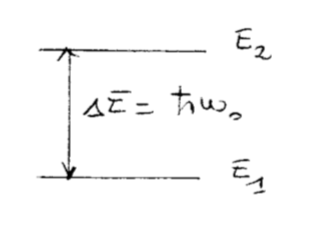
\includegraphics[width=0.9\linewidth]{jump}
\end{wrapfigure}

Consideriamo una collezione di atomi a due livelli di energia:  chiamiamo $E_1$ il primo livello, il quale è tipicamente il livello fondamentale dell'atomo, e $E_2 > E_1$ il secondo, che rappresenta lo stato eccitato con frequenza di risonanza:
\begin{equation*}
    \omega_0 \equiv \frac{E_2 - E_1}{\hbar}
\end{equation*}

Siano $N_1$ e $N_2$ le popolazioni atomiche, ovvero il numero di atomi per unità di volume sui livelli \lv{1} e \lv{2}. Si consideri poi un'onda e.m. monocromatica di frequenza $\omega$ che incide sulla collezione di atomi.\\
\\
Distinguiamo le varie casistiche.

\subsection{Assorbimento}

Qualitativamente il processo di assorbimento popola $N_2$ secondo la relazione:
\begin{equation*}
    \left( \frac{dN_2}{dt} \right)_{assorb.} = W_{12} N_1
\end{equation*}

\begin{wrapfigure}{R}{0.3\textwidth}
    \centering
    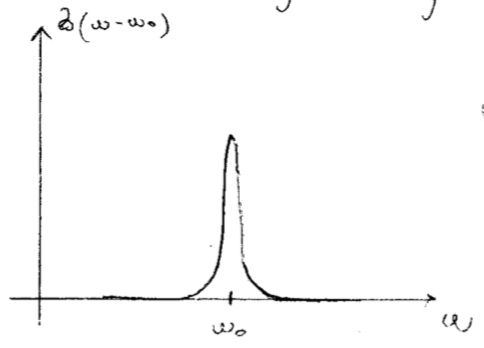
\includegraphics[width=0.9\linewidth]{deltad}
\end{wrapfigure}

dove, secondo la teoria semi-classica, il rate di assorbimento $W_{12}$ vale $W_{12} = \frac{I}{\hbar\omega} \cdot \sigma_{12}(\omega - \omega_0) = F \cdot \sigma_{12}(\omega - \omega_0)$ con $I$ l'intensità dell'onda incidente, $F = \frac{I}{\hbar\omega}$ il flusso fotonico e $\sigma_{12}(\omega -\omega_0)$ la \textit{cross-section} d'assorbimento della transizione \lv{1} $\leftrightarrow$ \lv{2} centrata in $\omega_0$.

La teoria semi-classica consente il calcolo di $\sigma_{12}$, la quale è quasi una delta di Dirac $\delta(\omega - \omega_0)$, cioè il processo di assorbimento di radiazione e.m. da parte di un atomo è un processo risonante il quale avviene solo se $\omega \approx \omega_0$. Ciò è giustificabile perché il processo di assorbimento deve conservare l'energia totale.

\subsection{Emissione stimolata}
\begin{wrapfigure}{R}{0.3\textwidth}
    \centering
    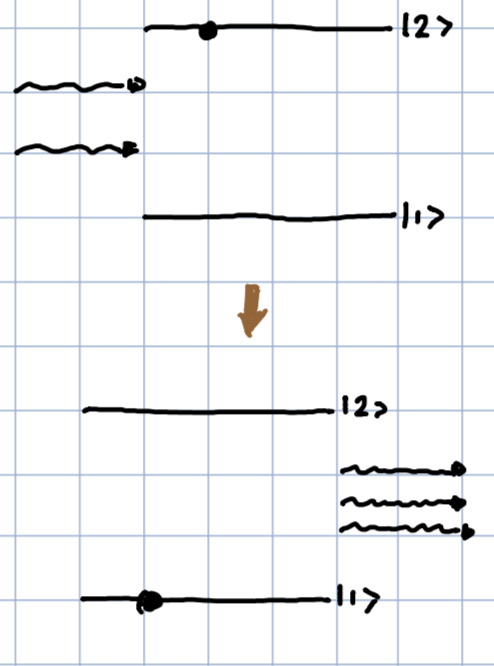
\includegraphics[width=0.9\linewidth]{emiss_stim}
    \caption{Emissione stimolata.}
\end{wrapfigure}

Un atomo nel livello \lv{2} che vede passare un fotone della giusta frequenza decade nel livello \lv{1} emettendo radiazione. Si crea un fotone identico: stesso modo, stessa frequenza, stessa polarizzazione etc. In tal caso possiamo scrivere secondo la teoria semi-classica:
\begin{equation*}
    \left( \frac{dN_2}{dt} \right) = W_{21} N_2
\end{equation*}

dove $W_{21} \equiv F \sigma_{21}(\omega - \omega_0)$.
Si dimostra che $W_{21} = W_{12}$ e quindi che $\sigma_{12} = \sigma_{21}$.\\

Cosa accade se su un atomo della popolazione $N_2$ non incide nessuna onda? Ci sono 2 possibilità.

\subsection{Emissione spontanea}

Un atomo inizialmente su \lv{2} in assenza di onde e.m. incidenti, spontaneamente, tende a decadere sul livello \lv{1}. Il modo spaziale, stato di polarizzazione, etc. del fotone emesso per emissione spontanea è casuale.\\
In tal caso:
\begin{equation*}
\left( \frac{dN_2}{dt} \right)_{\substack{emiss.\\ spont.}} = -\frac{N_2}{\tau_{spont.}}
\end{equation*}
con $\tau_{sp}$ si indica il tempo di vita \textit{radiativo} del livello eccitato \lv{2}.\\
Il decadimento nello spazio radiativo vuoto è dovuto alle fluttuazioni di energia di punto zero.

\subsection{Decadimento non-radiativo}

Un atomo in stato eccitato può decadere su un livello energetico inferiore mediante processi collisionali con altri atomi, senza emissione di fotone. L'energia interna dell'atomo può essere trasferita al partner urtante come energia cinetica (collisioni super elastiche), ceduto come energia interna oppure come ceduto ai fononi reticolari (nei solidi).\\
\\
Generalmente scriviamo:
\begin{equation*}
    \frac{dN_2}{dt} = - \frac{N_2}{\tau_{\text{non rad.}}}
\end{equation*}
dove $\tau_{\text{non rad.}}$ è il tempo di vita \textit{non radiativo} del livello eccitato \lv{2}.

\section{Assorbimento e amplificazione della luce}

Si consideri un'onda piana monocromatica di frequenza $\omega$ che si propaga in un mezzo materiale costituito da una collezione di atomi a due livelli.

\begin{wrapfigure}{R}{0.4\textwidth}
    \centering
    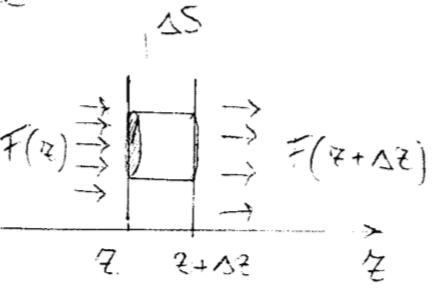
\includegraphics[width=0.9\linewidth]{flux}
\end{wrapfigure}

Siano $I(z)$, e $I(z + \Delta z)$ rispettivamente le intensità dell'onda in $z = z_0$ e $z = z_0 + \Delta z$.\\
Nel volume $\Delta V = \Delta S \Delta z$ si ha che il numero di fotoni distrutti nel volume $\Delta V$ nell'intervallo di tempo $\Delta t$ è pari a:
\begin{equation*}
    W_{12} N_1 \Delta V \Delta t
\end{equation*}
e che il numero di fotoni creati nel volume $\Delta V$ nell'intervallo di tempo $\Delta t$ è:
\begin{equation*}
    W_{21} N_2 \Delta V \Delta t
\end{equation*}

Deve quindi valere il seguente bilancio fotonico:
\begin{equation*}
    F(z + \Delta z) \Delta S \Delta t - F(z) \Delta S \Delta t = \underbrace{W_{12} N_1 \Delta V \Delta t}_\text{emissione stimolata} - \underbrace{W_{21} N_2 \Delta V \Delta t}_\text{assorbimento}
\end{equation*}

Siccome $W_{12} = W_{21} = \sigma(\omega - \omega_0) F$ si ha:
\begin{equation*}
    F(z + \Delta z) \Delta S \Delta t - F(z) \Delta S \Delta t = \sigma F(N_2 - N_1) \Delta z
\end{equation*}

quindi al limite per $\Delta z \rightarrow 0$:
\begin{equation*}
    \frac{dF}{dz} = \sigma \Delta N F \quad \text{con} \quad \Delta N \equiv N_2 - N_1 \quad \text{detta inversione di popolazione}
\end{equation*}

Dato che $F = \frac{I}{\hbar \omega}$ allora si ha che $\frac{dI}{dz} = \s \D N I$.\\
Supponendo $\Delta N$ indipendente da $z$ e da $I$\footnote{In generale non è vero a causa del fenomeno di saturazione.} si ha:
\begin{equation*}
    I(z) = I(0) e^{\sigma \Delta N z}
\end{equation*}

Distinguiamo due casi:

\begin{itemize}
    \item $N_1 > N_2$ cioè $\Delta N < 0$. Posto $\alpha \equiv (N_1 - N_2) \sigma$, il coefficiente di assorbimento del materiale, si ha:
    \begin{equation*}
        I(z) = I(0) e^{-\alpha z}
    \end{equation*}
    In questo caso, il mezzo è un assorbitore.
    \item $N_1 < N_2$ cioè $\Delta N > 0$. Posto $g \equiv (N_2 - N_1) \sigma$, il coefficiente di guadagno del materiale, si ha:
    \begin{equation*}
        I(z) = I(0) e^{g z}
    \end{equation*}
    In questo caso il mezzo è un amplificatore di luce.
\end{itemize}

Si noti che, all'equilibrio termodinamico a temperatura T, la distribuzione delle popolazioni atomiche è dato dalla distribuzione di Boltzmann:
\begin{equation*}
    \frac{N_2}{N_1} = e^{-\frac{E_2 - E_1}{k_B T}} = e^{-\frac{\hbar \omega_0}{k_B T}} < 1
\end{equation*}

Si tratta del caso $N_1 > N_2$ per cui non c'è inversione di popolazione. Per ottenere un amplificatore di luce si deve destabilizzare la distribuzione delle popolazioni con un meccanismo detto di \textit{pompaggio}. Generalmente, nei laser, si tratta di pompaggio elettrico oppure ottico.

\section{Principi e funzionamenti del laser}
Schema di un laser:
\begin{figure}[H]
    \centering
    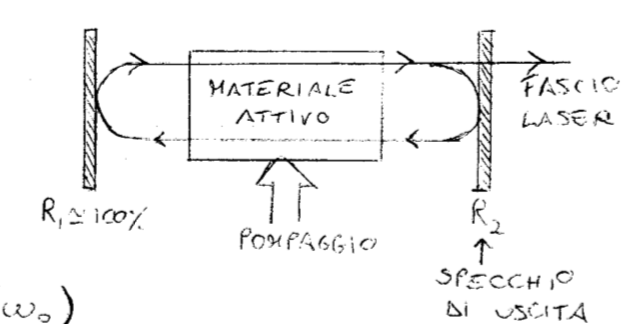
\includegraphics{schema_laser}
\end{figure}
dove indichiamo con $R_1$ e $R_2$ rispettivamente le riflettività degli specchi e con $l$ le dimensioni della cavità.\\
\\
Consideriamo un certo numero di fotoni nella cavità emessi per emissione spontanea.\\
Sia $F_1$ il flusso fotonico iniziale 
Nei successivi pompaggi all'interno della cavità il flusso fotonico si modifica così:
\begin{align*}
    & F_2 = F_1 e^{gl} \quad \text{con} \quad g \equiv (N_2 - N_1) \sigma = \sigma \Delta N\\
    & F_3 = R_2 F_2 = R_2 F_1 e^{gl}\\
    & F_4 = F_3 e^{gl} = R_2 F_1 e^{2gl}\\
    & F_5 = R_1 F_4 = R_1 R_2 F_1 e^{2gl}
\end{align*}

Introdotte le perdite logaritmiche $\gamma$ del risonatore:
\begin{equation*}
    \gamma \equiv -\frac{1}{2} \left[\ln (R_1) + \ln (R_2) \right] \qquad \rightarrow \qquad R_1 R_2 = e^{-2 \gamma}
\end{equation*}

si ha:
\begin{equation*}
    F_5 = F_1 e^{2(gl - \gamma)}
\end{equation*}

Quanto appena detto è valido per un \textit{round trip}.

\begin{figure}[H]
    \centering
    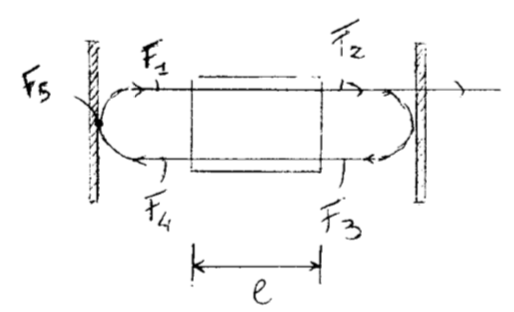
\includegraphics[width=10cm, height=4cm]{flux_schema_laser}
\end{figure}

All'n-esimo round trip si ha evidentemente:

\begin{equation*}
    F^{(n)} = F^{(0)} e^{2n(gl - \gamma)} \qquad n = 1, 2, 3, ...
\end{equation*}

Si distinguano quindi due casi:
\begin{itemize}
    \item laser \textbf{sotto-soglia} ($\gamma > gl$)\\
    Se $\gamma > gl$ allora $\gamma > \s \D N l$ e quindi $\D N < \frac{\gamma}{\sigma l}$ e $F^{(n)} \rightarrow 0$ ovvero il fotone emesso per emissione spontanea non riesce ad innescare la reazione a catena in cavità.
    \item laser \textbf{sopra-soglia} ($\gamma \leq gl$)\\
    Se $\gamma \leq gl$ allora $\D N > \s \D N_{th}$ dove per definizione $\D N_{th} \equiv \frac{\gamma}{\s l}$ detta \textit{inversione di popolazione critica} o di soglia.
\end{itemize}

\section{Meccanismo di pompaggio}

\subsection{Laser a due livelli}

\begin{figure}[H]
    \centering
    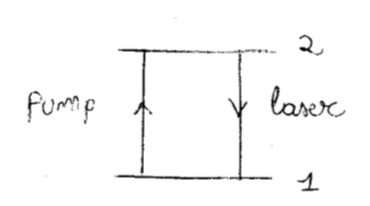
\includegraphics[width=4cm]{due_livelli}
\end{figure}

Questo tipo di laser non funziona. Al massimo si possono ottenere con metodi di pompaggio convenzionali $N_2 \leq N_1$ (trasparenza $N_2 = N_1$) ma mai $N_2 > N_1$

\subsection{Laser a tre livelli}

\begin{figure}[H]
    \centering
    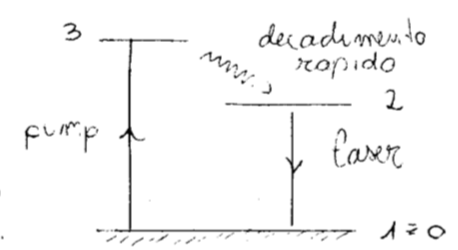
\includegraphics[width=4cm]{tre_livelli}
\end{figure}

Questo tipo di laser invece funziona ma non è ottimale, infatti per avere inversione di popolazione serve invertire più della metà degli atomi.

\subsection{Laser a quattro livelli}

\begin{figure}[H]
    \centering
    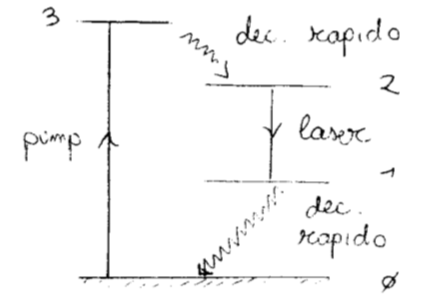
\includegraphics[width=4cm]{quattro_livelli}
\end{figure}

Questa è la soluzione ottimale perché è sufficiente invertire solo un atomo per avere inversione di popolazione.

\section{Proprietà della luce laser}

\begin{itemize}
    \item coerenza temporale (monocromaticità)
    \item coerenza spaziale
    \item direzionalità
    \item brillanza
    \item generazione di impulsi brevi
\end{itemize}
% Teoria semiclassica dell'interazione radiazione-materia
\chapter{Teoria semiclassica dell'interazione radiazione-materia}
\graphicspath{{./cap_2/images/}}

\section{Transizioni elettroniche indotte da perturbazioni dipendenti dal tempo}
Consideriamo l'atomo idrogenoide e indichiamo con $\psi(\*r,t)$ la funzione d'onda dell'elettrone più esterno (elettrone ottico) che compie transizioni. Trascuriamo lo spin dell'elettrone.\\
In assenza di perturbazioni $\psi$ evolve secondo l'equazione:
\begin{equation*}
    i\hbar \frac{\p \psi}{\p t} = \widehat{H}_0 \psi \quad \text{con} \quad \widehat{H}_0 \equiv -\frac{\hbar^2}{2m} \N^2 + V(\*r)
\end{equation*}

Indichiamo con $\lve{n} \equiv u_n(\*r)$ ed $E_n$ le autofunzioni normalizzabili (stati legati dell'atomo) e le energie (autovalori) di $\widehat{H}_0$:
\begin{equation}\label{eq: eq auto non perturbata}
    \widehat{H}_0 \lve{n} = E_n \lve{n}
\end{equation}

Ricordiamo che:
\begin{equation*}
    \langle n | m \rangle \equiv \intinf u_n^*(\*r) \; u_m(\*r) \; d\*r = \delta_{n,m} = \begin{cases}
        1\quad n = m\\
        0 \quad n \neq m
    \end{cases}
\end{equation*}

Supponiamo che l'elettrone interagisca con una perturbazione esterna (ad esempio, l'atomo è investito da un'onda e.m.). La perturbazione è descritta da un operatore auto-aggiunto $\hat{H_p}$ che assumiamo della forma:
\begin{equation}\label{eq: ham perturbata}
    \widehat{H}_p = f(t) \widehat{p}
\end{equation}

dove $f(t)$ è in funzione quasi monocromatica nel tempo della forma seguente:
\begin{equation*}
    f(t) = \frac{1}{2} \left[ A(t) e^{i\w t} + c.c. \right]
\end{equation*}
con $A(t)$ lentamente variabile di periodo $T =  \frac{2\pi}{\omega}$.

$\widehat{p}$ è un operatore indipendente dal tempo che quindi agisce sulle sole coordinate spaziali $\*r$.\\
In presenza della perturbazione l'equazione di Schr\"{o}dinger diventa:
\begin{equation} \label{eq: schrod perturbata}
    i\hbar \frac{\p \psi}{\p t} = \left(\widehat{H}_0 + \widehat{H}_p\right)\psi
\end{equation}

essendo $\widehat{H} = \widehat{H}_0 + \widehat{H}_p$ l'hamiltoniana complessiva.\\
Se si trascurano i processi di ionizzazione, ad ogni istante $t$, $\psi(\*r,t)$ può essere sviluppata in serie degli autostati \lv{n} di $\widehat{H}_0$ cioè:
\begin{equation}\label{eq: fun donda}
    \psi(\*r,t) = \sum_n C_n(t) e^{-i\frac{E_n}{\hbar}t} \lve{n}
\end{equation}

Sostituendo l'\textit{Ansatz} (assunzione) \eqref{eq: fun donda} nella \eqref{eq: schrod perturbata} si ha:
\begin{equation*}
    i\hbar \sum_n \left[\frac{d C_n}{d t} - i\frac{E_n}{\hbar} C_n \right] e^{-i\frac{E_n}{\hbar}t} \lve{n} = \sum_n C_n [\widehat{H}_0 + \widehat{H}_p] e^{-i\frac{E_n}{\hbar}t} \lve{n}
\end{equation*}

\begin{equation*}
    i\hbar \sum_n \dot{C}_n e^{-i\frac{E_n}{\hbar}t} \lve{n} + \cancel{i\hbar \sum_n C_n e^{-i\frac{E_n}{\hbar}t} \left(-i\frac{E_n}{\hbar}\right) \lve{n}} = \cancel{\sum_n C_n e^{-i\frac{E_n}{\hbar}t} \widehat{H}_0 \lve{n}} + \sum_n C_n e^{-i\frac{E_n}{\hbar}t} \widehat{H}_p \lve{n}
\end{equation*}

sostituendo \eqref{eq: eq auto non perturbata}, \eqref{eq: ham perturbata} e semplificando si ottiene:
\begin{equation*}
    i\hbar \sum_n \dot{C}_n e^{-i\frac{E_n}{\hbar}t} \lve{n} = \sum_n C_n e^{-i\frac{E_n}{\hbar}t} f(t) \widehat{p} \lve{n}
\end{equation*}

Moltiplicando per $\langle m|$ e tenendo conto che $\langle m|n\rangle = \delta_{n,m}$ si ha:
\begin{equation*}
    i\hbar \dot{C}_m e^{-i\frac{E_m}{\hbar}t} = f(t) \sum_n \langle m|\widehat{p}|n\rangle C_n e^{-i\frac{E_n}{\hbar}t}
\end{equation*}

ovvero:
\begin{equation*}
    i\hbar \dot{C}_m = f(t) \sum_n p_{m,n} C_n e^{-i\frac{(E_n - E_m)}{\hbar}t}
\end{equation*}

avendo posto:
\begin{equation*}
    p_{m,n} \equiv \langle m|\widehat{p}|n\rangle \equiv \intinf u_m^*(\*r) \; \widehat{p} \; u_n(\*r) \; d\*r
\end{equation*}
definito elemento di matrice di perturbazione.\\

Si noti che $p_{n,m}$ è una matrice hermitiana, ovvero $p_{n,m} = p_{n,m}^*$.\\
\\
\textit{Qual è il significato fisico di $C_n(t)$?}
\begin{indentedpar}{1cm}
$|C_n(t)|^2$ è la probabilità che al tempo $t$ l'elettrone si trovi sullo stato \lv{n} con energia $E_n$.
\end{indentedpar}
\noindent
\textit{Qual è l'effetto della perturbazione?}
\begin{indentedpar}{1cm}
Se non ci fosse la perturbazione, cioè se $f(t) = 0$ allora $|C_n(t)|^2 = cost$.
Quindi, se al tempo $t=0$ l'elettrone, con certezza, si trova su un dato livello $\bar{n}$ cioè $C_n(0) = \delta_{n,\bar{n}}$ allora l'elettrone rimane sul livello \lv{\bar{n}} (stato stazionario).

In presenza di una perturbazione i $C_n(t)$ variano nel tempo. La perturbazione induce cioè transizioni tra i diversi stati stazionari dell'atomo.
\end{indentedpar}

Fissando l'attenzione al caso dell'atomo a due livelli \lv{1} e \lv{2}, chiamando $\omega_0 = \frac{E_2 - E_1}{\hbar}$ la frequenza di risonanza della transizione $\lve{1} \leftrightarrow \lve{2}$ e notando che gli elementi diagonali della matrice di perturbazione $p_{1,1}$ e $p_{2,2}$ sono nulli si ha:
\begin{empheq}[box=\eqbox]{equation*}
    \begin{cases}
        i\hbar \dot{C_1} = f(t) \; p_{12} \; C_2 \; e^{-i\omega_0 t} \qquad \textbf{equazione del sistema}\\
        i\hbar \dot{C_2} = f(t) \; p_{21} \; C_1 \; e^{i\omega_0 t} \qquad \textbf{ di un atomo a due livelli}
    \end{cases}
\end{empheq}

Specifichiamo le condizioni iniziali per una perturbazione piccola.\\
Si supponga che al tempo $t=0$ l'elettrone sia con certezza sul livello \lv{2} e che  quindi $C_1(0) = 0$ e $C_2(0) = 1$ e, inoltre, si supponga che la perturbazione sia quasi monocromatica con frequenza $\w\simeq\omega_0$ ovvero $f(t) = \frac{1}{2} \left( A(t) e^{-i\omega t} + \,c.c.\right)$ con $A(t)$ lentamente variabile su un intervallo $\frac{2\pi}{\omega}$.

Se la perturbazione è debole (ovvero se $A \rightarrow 0$) e se il tempo di interazione ($0,t$) non risulta troppo grande allora $C_1(t)$ e $C_2(t)$ non varieranno troppo rispetto ai valori imperturbati, ovvero:
\begin{equation*}
    |C_1(t)|^2 << 1 \qquad |C_2(t)|^2 \simeq 1
\end{equation*}

Possiamo in tale ipotesi trascurare la seconda equazione nel sistema e risolvere la prima:
\begin{equation*}
    i\hbar \dot{C_1} = p_{1,2} \; f(t) \; C_2 \; e^{-i\omega_0 t} \approx p_{1,2} \; f(t) \; e^{-i\omega_0 t}
\end{equation*}

deducendo che l'evolvere di $C_1$ non dipende da $C_2$.
Risolvendo per $C_1(t)$ si ottiene:
\begin{equation*}
    C_1(t) = \frac{p_{1,2}}{i\hbar} \int_0^t f(t') \; e^{-i\omega_0 t'} dt'
\end{equation*}

Se spengo la perturbazione al tempo $t = T$ la probabilità di trovare l'elettrone sul livello \lv{1} vale:
\begin{equation}\label{eq: probab c1}
    |C_1(t)|^2 = \frac{|p_{1,2}|^2}{\hbar^2} \left|\int_0^T f(t') \; e^{-i\omega_0 t'} dt'\right|^2
\end{equation}

È quindi possibile introdurre una\textbf{ probabilità di transizione} $W_{21}$ da $\lve{2} \rightarrow \lve{1}$ nell'unità di tempo così definita:
\begin{equation*}
    W_{21} = \lim_{T \rightarrow \infty} \frac{|C_1(T)|^2}{T}
\end{equation*}

Sostituendo $f(t) = \frac{1}{2} \left[ A(t) e^{-i\omega t} + c.c.\right]$ nell'integrale della \eqref{eq: probab c1} si ha:
\begin{equation*}
    \left|\int_0^T f(t') e^{-i\omega_0 t'} dt'\right|^2 = \left|\underbrace{\frac{1}{2} \int_0^T A(t') e^{i(\omega - \omega_0) t'} dt'}_\text{termine risonante} + \underbrace{\frac{1}{2} \int_0^T A^*(t') e^{-i(\omega + \omega_0) t'} dt'}_\text{termine anti-risonante} \right|^2
\end{equation*}

\textbf{Nota.}\\
Se $A(t) = 1$ e $\omega = \omega_0$ si hanno:
\begin{equation*}
    \int_0^T  dt' = T \quad \text{termine risonante}
\end{equation*}
\begin{equation*}
    \int_0^T e^{-2i\omega_0 t'} dt' = \frac{1 - e^{-2i\omega_0 T}}{2i \omega_0} \quad \text{termine anti-risonante}
\end{equation*}

Trascurare il termine anti-risonante è detta \textbf{approssimazione di onda rotante}.
Facendo questa approssimazione quindi si ottiene:
\begin{empheq}[box=\eqbox]{equation}\label{eq: regola di fermi}
    W_{21} = \frac{|p_{1,2}|^2}{4\hbar^2} S(\omega - \omega_0) \quad \text{regola d'oro di Fermi}
\end{empheq}

avendo posto:
\begin{empheq}[box=\eqbox]{equation*}
    S(\D \w) \equiv \lim_{T \rightarrow \infty} \frac{1}{T} \left| \int_0^T A(t') e^{i(\D\w) t'} dt' \right|^2 \quad \text{spettro di potenza dell'inviluppo A(t)}
\end{empheq}

\textbf{Osservazioni.}
\begin{enumerate}
    \item Se $C_1(0) = 1$ e $C_2(0) = 0$ applicando la matrice di perturbazione si ha che:
    \begin{equation*}
        W_{12} = \lim_{T \rightarrow \infty} \frac{|C_2(T)|^2}{T} = W_{21}
    \end{equation*}

    \item Un altro metodo per scrivere la Regola d'oro di Fermi è attraverso le funzioni di autocorrelazione:
    \begin{equation*}
        A_T(t) = \begin{cases}
            A(t) \quad 0 < t < T\\
            0 \quad \text{altrimenti} 
        \end{cases}    
    \end{equation*}
    e la funzione di autocorrelazione:
    \begin{equation*}
        R(t) \equiv \intinf A_T(t) A_T^*(t - \tau) dt
    \end{equation*}
    allora è facile vedere che:
    \begin{equation*}
        S(\D\w) = \intinf R(\tau) e^{i\D\w\tau} d\tau
    \end{equation*}
    ovvero lo spettro di potenza $S(\D\w)$ di $A(t)$ è l'integrale di Fourier della sua funzione di autocorrelazione.
    
    \item La teoria di perturbazione è valida quando è verificata la seguente condizione:
    \begin{equation*}
        W_{21}T << 1
    \end{equation*}
    infatti:
    \begin{equation*}
        W_{21} = \frac{|C_1(T)|^2}{T} \Longrightarrow |C_1(T)|^2 = W_{21}T << 1
    \end{equation*}
\end{enumerate}

\begin{example}
Perturbazione rigorosamente monocromatica.\\
Supponiamo $f(t) = \cos(\omega t)$ cioè $A(t) = 1$. In tal caso lo spettro di potenza $S$ vale:
\begin{align*}
    S(\D \w) &= \lim_{T \rightarrow \infty} \frac{1}{T} \left| \int_0^T e^{i(\D\w) t} dt \right|^2\\
    &= \lim_{T \rightarrow \infty} \frac{1}{T} \left|\frac{e^{i\D\omega T} - 1}{i\D w} \right|^2\\
    &= \lim_{T \rightarrow \infty} \frac{1}{T} \left|\frac{e^{\frac{i\D\omega T}{2}} \left(e^{\frac{i\D\omega T}{2}} - e^{\frac{-i\D\omega T}{2}} \right)}{i\D w} \right|^2\\
    &= \lim_{T \rightarrow \infty} \frac{1}{T} \left|\frac{4 \sin^2\left(\frac{\D\omega T}{2}\right)}{\D w^2} \right|^2\\
    &= \lim_{T \rightarrow \infty} T \left|\frac{\sin^2\left(\frac{\D\omega T}{2}\right)}{\left(\frac{\D w T}{2}\right)^2} \right|^2
\end{align*}

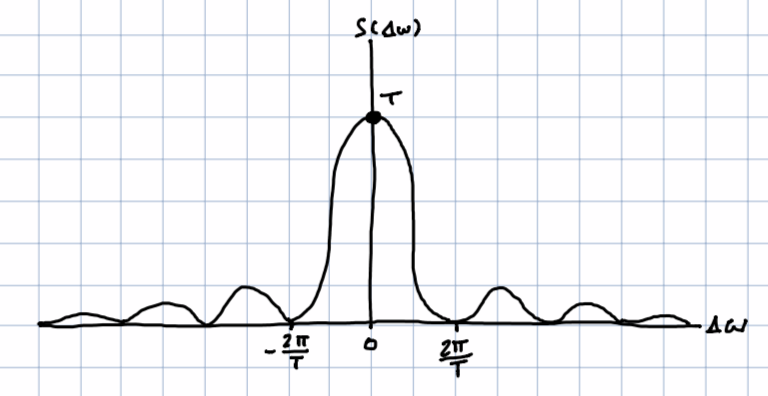
\includegraphics[width=5cm, center]{sinc}

Studiamo la funzione $G(\D \w) = T sinc^2\left(\frac{\D \omega T}{2}\right)$ al crescere di T.

Si noti che l'area:
\begin{equation*}
    \intinf G(\D \w) = T \intinf sinc^2\left(\frac{\D \omega T}{2}\right) = T \frac{2}{T} \intinf \frac{sin^2\xi}{\xi^2} d\xi = 2\pi
\end{equation*}

Nel limite $T \rightarrow \infty$:
\begin{equation*}
    G(\D \w) = \begin{cases}
        \infty \quad \D\omega = 0\\
        0 \quad \D\omega \neq 0
    \end{cases}
\end{equation*}
cioè lo spettro di potenza tenderà ad una delta di Dirac di area $2\pi$ per $\Delta \omega \rightarrow 0$.

In definitiva $\Delta S(\Delta \w) = 2\pi \delta(\Delta \w)$:
\begin{equation*}
    W_{12} = W_{21} = \pi \frac{|p_{1,2}|^2}{2\hbar^2} \delta(\omega - \omega_0) \quad \text{per perturbazione monocromatica}
\end{equation*}
\end{example}

\begin{example}Onda quasi monocromatica con salti di fase casuali\\
Supponiamo che $f(t) = \cos(\omega t +\varphi(t))$ con $\varphi(t)$ costante a tratti con discontinuità a valori casuali distribuiti fra $(0,2\pi)$, ad intervalli $\tau$ con $\tau$ variabile aleatoria. 
\begin{wrapfigure}{R}{0.3\textwidth}
    \centering
    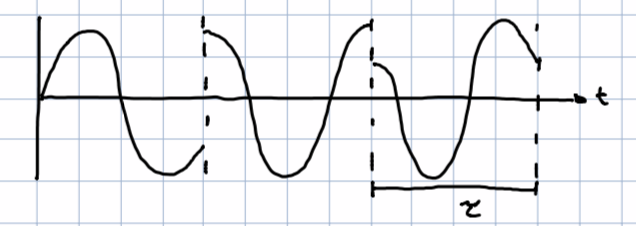
\includegraphics[width=0.9\linewidth]{phase_jumps}
\end{wrapfigure}
Supponiamo inoltre che $\varphi$ abbia distribuzione di probabilità esponenziale:
\begin{equation*}
    \varphi(\tau) = \frac{1}{\tau_c} e^{-\frac{\tau}{\tau_c}}
\end{equation*}
dove $\tau_c$ è il valore medio.

Calcoliamo lo spettro di potenza $S(\D \w)$ come integrale di Fourier della funzione di autocorrelazione $R(\tau)$\footnote{Per il calcolo di $R(\tau)$ vedi \textit{Principles of lasers} Appendice del capitolo 12}.

Il risultato è:
\begin{equation*}
R(\tau) = e^{-\frac{|\tau|}{\tau_c}}
\end{equation*}
%grafico
Calcolo lo spettro di potenza:
\begin{align*}
    S(\D \w) &= \intinf e^{-\frac{|\tau|}{\tau_c}} e^{i\D\w\tau} d\tau\\
    &= \int_0^{+\infty} e^{-\frac{|\tau|}{\tau_c}} e^{i\D\w\tau} d\tau + \int_{-\infty}^0 e^{\frac{|\tau|}{\tau_c}} e^{i\D\w\tau} d\tau\\
    &= \frac{e^{\left(i\D\omega - \frac{1}{\tau_c}\right)\tau|_0^{+\infty}}}{i\D\omega - \frac{1}{\tau_c}} + \frac{e^{\left(i\D\omega + \frac{1}{\tau_c}\right)\tau|_{-\infty}^0}}{i\D\omega + \frac{1}{\tau_c}}\\
    &= -\frac{1}{i\D\omega - \frac{1}{\tau_c}} + \frac{1}{i\D\omega + \frac{1}{\tau_c}}\\
    &= \frac{\tau_c}{1 - i\D\w\tau_c} + \frac{\tau_c}{1 + i\D\w\tau_c}\\
    &= \frac{2\tau_c}{1 + (\D\w\tau_c)^2}
\end{align*}

che possiamo riscrivere:
\begin{equation*}
    S(\D\w) = 2\pi g_L(\D\w)
\end{equation*}

dove:
\begin{empheq}[box=\eqbox]{equation*}
    g_L\left(\D\w\right) = \frac{\tau_c}{\pi} \frac{1}{1 + (\D\omega \tau_c)^2} \quad \text{funzione lorentziana}
\end{empheq}

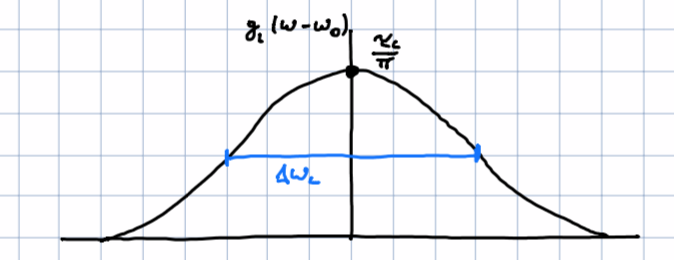
\includegraphics[width=5cm, center]{lorentziana}

È quindi facile vedere che $g_L$ è normalizzata: $\intinf g_L(\D\w) d\D\omega = 1$.

La lunghezza a metà altezza $FWHM$ della lorentziana vale:
\begin{equation*}
    g_L\left(\frac{\D\omega_L}{2}\right) = \frac{\tau_c}{2\pi}
\end{equation*}
ovvero vale
\begin{equation*}
    \D \omega_L = \frac{2}{\tau_c}
\end{equation*}
Pertanto per la regola d'oro di Fermi \eqref{eq: regola di fermi}
\begin{equation*}
    W_{12} = W_{21} = \frac{|p_{1,2}|^2}{4\hbar^2} S(\omega - \omega_0)
\end{equation*}

Il caso di onda perfettamente monocromatica è per la lorentziana il limite $\tau_c \rightarrow \infty$.\\
Ritroviamo il risultato dell'esempio.

L'espressione $W_{12} = W_{21}$ dalla teoria perturbativa è ben posta anche a risonanza ($\omega = \omega_0$) in quanto la lorentziana non ha la singolarità del seno cardinale.
\end{example}

\section{Assorbimento ed emissione stimolata: Calcolo di $W_{12} = W_{21}$}
Considero un atomo a due livelli investito da un'onda piana (quasi) monocromatica di frequenza $\w$, che si propaga nella direzione $z$ dello spazio con campo $\*E$ linearmente polarizzato in direzione $x$.

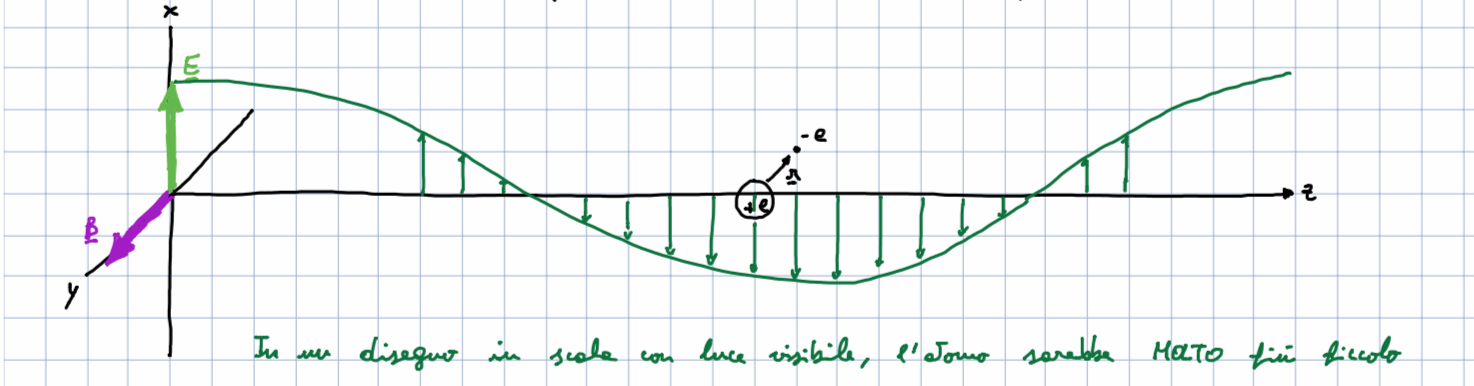
\includegraphics[width=12cm, center]{onda_mono_lin_pol}

L'elettrone dell'atomo risente, oltre che del potenziale nucleare, anche della forza di Lorentz:
\begin{equation*}
    \*F = -e\*E - e\*v\times\*B = -e\*E_x(z, t)\*u_x -e\*v\times \*u_y\*B_y(z, t)
\end{equation*}
L'hamiltoniana classica per un elettrone in un campo elettromagnetico è la seguente:
\begin{equation*}
    \widehat{H} = \frac{1}{2m} \left(\*p + q\*A\right)^2 + qV \qquad \N\cdot\*B = \N\cdot\N\times\*A = 0
\end{equation*}

Nell'approssimazione di dipolo elettrico assumiamo le seguenti ipotesi:
\begin{enumerate}
    \item Poiché l'elettrone è localizzato attorno al nucleo per una dimensione dell'ordine del raggio di Bohr $a_0 \propto 0.053 nm$ e la lunghezza d'onda nel visibile (rosso) è circa $\l \simeq 500 nm$ allora possiamo considerare il campo elettrico e il campo magnetico pressoché costanti. Posso quindi assumere, nell'espressione di $\*F$, $z=z_N$. Ovvero la coordinata $z$ è costante e pari alla posizione del nucleo.
    
    \item Per basse velocità $|\*v| << c$ è possibile trascurare la forza di Lorentz.
\end{enumerate}

Per queste ipotesi si ha che la forza che l'elettrone sente per effetto dell'onda e.m. è pari a:
\begin{equation}
    \*F(t) \simeq -e\*E_x(z_N, t)\*u_x
\end{equation}
la quale deriva dall'energia potenziale $H_p(x, t) = e x E_x(t)$.

Si noti che l'energia classica di dipolo elettrico in campo esterno è la seguente:
\begin{equation}
    H_p -\*{\mu} \cdot \*E
\end{equation}
dove $\*\mu = -e\*r$ è il momento di dipolo elettrico dell'atomo.

L'operatore quantistico di perturbazione è pertanto:
\begin{equation}
    \hat{H}_p = e x E_x(t) = f(t) \hat{p}
\end{equation}
dove $f(t) = E_x(t)$ e $\hat{p} \equiv e x = -\*\mu \cdot \*u_x$.

L'elemento di matrice di perturbazione che entra nella formula di $W_{12} = W_{21}$
\begin{equation}
    |p_{12}|^2 = |<1|e x|2>|^2 = \left|\intinf u_1^*(\*r) \; e x \; u_1(\*r) d\*r \right|^2
\end{equation}
ovvero $|p_{12}|^2 = |\mu_{12x}|^2$
dove si è definito l'elemento di matrice di dipolo elettrico della transizione $\lve{1} \rightarrow \lve{2}$:
\begin{equation}
    \*\mu_{12} \equiv <1|e\*r|2>
\end{equation}

Quindi, ad esempio, per onda rigorosamente monocromatica, cioè se $E_x(t) = E_x \cos(\w t)$:
\begin{equation}
    W_{12} = W_{21} = \frac{\pi |\mu_{12x}|^2 E_0^2}{2 \hbar^2} \delta(\w - \w_0)
\end{equation}

Se invece $E_x(t) = E_0 \cos(\w t + \varphi(t))$ similmente si ha:
\begin{equation}
    W_{12} = W_{21} = \frac{\pi |\*\mu_{12x}|^2 E_0^2}{2 \hbar^2} g_L(\w - \w_0)
\end{equation}
Nel caso si abbiano più atomi, il valore medio vale:
\begin{equation}
    \bar{W}_{12} = \bar{W}_{21} = \frac{\pi <|\*\mu_{12x}|^2> E_0^2}{2 \hbar^2} g_L(\omega - \omega_0)
\end{equation}
dove $<|\*\mu_{12x}|^2>$ è il valore medio $\frac{|\*\mu_{12x}^{(1)}|^2 + |\*\mu_{12x}^{(2)}|^2 + ... + |\*\mu_{12x}^{(n)}|^2}{N}$.

Se la distribuzione degli atomi nello spazio è isotropa:
\begin{equation}
    <|\*\mu_{12x}|^2> = <|\*\mu_{12y}|^2> = <|\*\mu_{12z}|^2>
\end{equation}

Del resto $|\*\mu_{12x}|^2 + |\*\mu_{12y}|^2 + |\*\mu_{12z}|^2 = |\*\mu_{12}|^2$ quindi mediando:
\begin{equation}
    <|\*\mu_{12x}|^2> + <|\*\mu_{12y}|^2> + <|\*\mu_{12z}|^2> = |\*\mu_{12}|^2
\end{equation}
e quindi:
\begin{equation}
    <|\mu_{12x}|^2> = \frac{|\mu_{12}|^2}{3}
\end{equation}

In definitiva:
\begin{empheq}[box=\eqbox]{equation*}
    W_{12} = W_{21} = \frac{\pi |\*\mu_{12}|^2 E_0^2}{6 \hbar^2} g_L(\w - \w_0)
\end{empheq}
Per tenere conto di tanti atomi è sufficiente dividere per 3 il modulo di $\*\mu_{12}$.

Con questa teoria si può studiare l'effetto sull'atomo della perturbazione dell'onda ma non è possibile sapere cosa succede all'onda (fotone creato, distrutto); per tenere conto di ciò è necessaria la teoria di seconda quantizzazione.

\textbf{Osservazioni.}\\
\begin{enumerate}
    \item Regole di selezione di dipolo elettrico:
    $W_{12} = W_{21}$ si annulla se l'elemento di matrice di transizione $ = 0$. In tal caso la transizione si dice proibita per dipolo elettrico, altrimenti è permessa.
    Negli atomi idrogenoidi $\hat{H}_0(-\*r) = \hat{H}_0(\*r)$ cioè è simmetrica per invarianza, per cui le autofunzioni $u_n(\*r) \equiv \lve{n}$ sono a parità definita, cioè:
    \begin{equation}
        u_n(-\*r) = u_n(\*r) \quad pari \qquad u_n(-\*r) = - u_n(\*r) \quad dispari
    \end{equation}
    Per cui:
    \begin{equation}
        \*\mu_{12} = \intinf u_1^*(\*r) \; e \*r \; u_1(\*r) dx dy dz = \begin{cases}
        0 \quad \text{se \lv{1} e \lv{2} stessa parità}\\
        \neq 0 \quad \text{se \lv{1} e \lv{2} parità opposta}
        \end{cases}
    \end{equation}
    Ci può essere transizione solo per autofunzioni di parità opposta. Questa proprietà dà origine alle cosiddette \textit{Regole di Selezione}, che per atomi idrogenoidi sono:
    \begin{equation}
        \Delta l = \pm 1 \quad \Delta j = 0, \pm 1 \quad \Delta m_j = 0, \pm 1
    \end{equation}
    Ad esempio transizioni tra stati \textit{s} e \textit{p} sono permesse per dipolo elettrico (non c'è nessun vincolo su \textit{n}).
    Queste regole sono valide nelle ipotesi dell'approssimazione di dipolo elettrico.
    
    \item Transizioni indotte per dipolo magnetico\\
    Se $\*\mu_{12} = 0$, i processi di assorbimento / emissione stimolata possono avvenire per interazioni di ordine superiore
    Mi limito a studiare il dipolo magnetico, l'energia classica di interazione è:
    \begin{equation}
        H_p = - \*\mu_m \cdot \*B
    \end{equation}
    dove $\*\mu_m = IS \*n = -\frac{e S}{T} \*n$ è il momento di dipolo magnetico calssico dell'elettrone orbitale e $\*B$ è il campo magnetico dell'onda, dove $S$ è l'area dell'orbita e T il periodo di rivoluzione.
    Detta $\alpha$ la velocità angolare:
    \begin{equation}
        \alpha = \frac{1}{2} r^2 \frac{d\theta}{dt} = \frac{1}{2} r^2 \dot{\theta} = costante
    \end{equation}
    Quindi $S = \int_0^T \alpha dt = \alpha T$ per cui $\*\mu = -e \alpha \*n$.
    Il momento angolare dell'elettrone è $\*L = \*r \times m\*v = mr^2 \dot{\theta} \*n = 2m \alpha \*n$ quindi:
    \begin{equation}
        \*\mu_{m} = -\frac{e}{2m} \*L
    \end{equation}
    L'energia classica di interazione è quindi ($\*B = B_y \*\mu_y = B_0 cos(\w t + \varphi(t))$):
    \begin{equation}
        H_p = -\*mu \cdot \*B = \frac{e}{2m} L_y B_y
    \end{equation}
    L'hamiltoniana quantistica di perturbazione si ottiene quantizzando:
    \begin{equation}
        \hat{H}_p = \frac{e}{2m} \hat{L}_y B_y \equiv f(t) \hat{p}
    \end{equation}
    \begin{equation}
        f(t) = B_y(t) \quad \rightarrow \quad \hat{p} = \frac{e}{2m} \hat{L}_y = \frac{e\hbar}{2m} \frac{\hat{L}_y}{\hbar} = \mu_B \frac{\hat{L}_y}{\hbar}
    \end{equation}
    dove $\mu_B = \frac{e\hbar}{2m}$ è il magnetone di Bohr ovvero il quanto di interazione di dipolo magnetico.
    
    Applicando la teoria delle perturbazioni, si ottiene:
    \begin{equation}
        W_{12}^{magn} = W_{21}^{magn} = \frac{|p_{12}|^2 B_0^2}{2\hbar^2} g_L(\omega - \omega_0)
    \end{equation}
    con $|p_{12}|^2 = \mu_B^2 \left| <1|\frac{\hat{L}_y}{\hbar}\right|^2$.
    Se $\varphi(t) = 0$ allora $g_L \rightarrow \delta$.
    
    Calcoliamo l'ordine di grandezza del rapporto $\frac{W_{12}^{elec}}{W_{12}^{magn}}$:
    \begin{equation}
        \frac{W_{12}^{elec}}{W_{12}^{magn}} = \frac{|\mu_{12x}|^2 E_0^2}{B_0^2 \mu_B^2 \left| <1|\frac{\hat{L}_y}{\hbar}\right|^2} \simeq \left(\frac{c e a_B}{\mu_B}\right)^2 \simeq 10^5
    \end{equation}
    essendo $\left| <1| ex |2> \right|^2 \simeq (e a_B)^2$ e $\left| <1|\frac{\hat{L}_y}{\hbar}\right|^2 \simeq m^2 \simeq 1$, con $m$ numero quantico magnetico, il contributo della probabilità di transizione per dipolo magnetico, se permessa per dipolo elettrico, è trascurabile.
\end{enumerate}


\section{Teoria esatta dell'interazione coerente tra atomo a due livelli e radiazione. Oscillazioni di Rabi}

Considero l'interazione coerente (indisturbata) tra atomo a due livelli e onda e.m. quasi monocromatica.
Assumo la transizione $\lve{1} \rightarrow \lve{2}$ permessa per dipolo elettrico. Le equazioni esatte delle ampiezze di probabilità $C_1$ e $C_2$ sono:
\begin{equation}
    \begin{cases}
        i\hbar \dot{C_1} = \mu_{12x} \; E_x(t) \; C_2 \; e^{-i\omega_0 t}\\
        i\hbar \dot{C_2} = \mu_{21x} \; E_x(t) \; C_1 \; e^{i\omega_0 t}
    \end{cases}
\end{equation}
con $E_x(t) = \frac{1}{2} \left[ A(t) e^{i\w t} + c.c. \right]$
\begin{equation}
    \begin{cases}
        i\hbar \dot{C_1} =  \frac{\mu_{12x}}{2} \left[ A(t) e^{i (\w-\w_0) t} + \cancel{A^*(t)e^{-i (\w+\w_0) t}} \right] \; C_2\\
        i\hbar \dot{C_2} =  \frac{\mu_{21x}}{2} \left[ \cancel{A(t) e^{i (\w+\w_0) t}} + A^*(t)e^{-i (\w-\w_0) t} \right] \; C_1
    \end{cases}
\end{equation}
Nell'approssimazione di onda rotante i termini fuori dalla diagonale sono antirisonanti rapidamente oscillanti a valore medio nullo quindi si trascurano.

Nella RWA:
\begin{equation}
    \begin{cases}
        i\hbar \dot{C_1} \simeq  \frac{\mu_{12x}}{2}A(t) e^{i (\w-\w_0) t} \; C_2\\
        i\hbar \dot{C_2} \simeq  \frac{\mu_{21x}}{2} A^*(t)e^{-i (\w-\w_0) t} \; C_1
    \end{cases}
\end{equation}

Suppongo che al tempo $t = 0$ l'atomo sia nel livello \lv{1} quindi $C_1(0) = 1$ e $C_2(0) = 0$.

Studiamo 3 casi interessanti:
\begin{enumerate}
    \item $A(t) = E_0$ costante $\w = \w_0$ è il caso in cui $W_{12} \rightarrow \infty$ e la teoria di perturbazione è inconsistente.
    
    In tal caso, si definisce:
    \begin{empheq}[box=\eqbox]{equation*}
        \Omega_R \equiv \frac{\mu_{12x} E_0}{\hbar} \qquad \textbf{frequenza di Rabi} 
    \end{empheq}
    la misura, in unità di $\hbar$, dell'energia di interazione.
    
    Si ha:
    \begin{equation}
        \begin{cases}
            i\hbar \dot{C_1} \simeq  \frac{\mu_{12x}}{2}A(t) e^{i (\w-\w_0) t} \; C_2\\
            i\hbar \dot{C_2} \simeq  \frac{\mu_{21x}}{2} A^*(t)e^{-i (\w-\w_0) t} \; C_1
        \end{cases}
    \end{equation}
    Si noti che $C_1$ e $C_2$ soddisfano l'equazione dell'oscillatore armonico con $\omega = \frac{\Omega_R}{2}$:
    \begin{equation}
        \Ddot{C}_1 + \left(\frac{\Omega_R}{2}\right)^2 C_1 = 0
    \end{equation}
    La soluzione del sistema con le condizioni iniziali $C_1(0) = 1$ e $C_2(0) = 0$ è:
    \begin{equation}
        \begin{cases}
            C_1(t) = \cos\left(\frac{\Omega_R}{2}\right)
            C_2(t) = -i \sin\left(\frac{\Omega_R}{2}\right)
        \end{cases}
    \end{equation}
    
    Si noti che se avessi applicato la teoria di perturbazione avrei ottenuto $i\dot{C_2} \simeq \frac{\Omega_R}{2}$ cioè $C_2(t) = -i \frac{\Omega_R}{2} t$ e $$W_{12} = \lim_{T \to \infty} \frac{|C_2(t)|^2}{T} = \lim_{T \to \infty} \frac{|C_2(t)|^2}{T} \to \infty$$ il ché è inconsistente.
    %disegno
    Rappresenta uno scambio periodico di energia tra atomo e radiazione:\\
    $assorbimento \rightarrow emissione \rightarrow assorbimento \rightarrow emissione \rightarrow ...$
    
    \item  Oscillazione di Rabi $E = E_0$ costante $\w \neq \w_0$.
    \begin{equation}
        \begin{cases}
            i\hbar \dot{C_1} \simeq  \frac{\mu_{12x}}{2}A(t) e^{i (\w-\w_0) t} \; C_2\\
            i\hbar \dot{C_2} \simeq  \frac{\mu_{21x}}{2} A^*(t)e^{-i (\w-\w_0) t} \; C_1
        \end{cases}
    \end{equation}
    Integrando con le stesse condizioni iniziali considerate nel caso precedente:
    %disegno
    \begin{equation}
        T = \frac{2\pi}{\sqrt{\Omega_R^2 + (\w - \w_0)^2}}
    \end{equation}
    e $\Delta = \Delta(\omega - \omega_0) \to 0$ se $\left|\frac{\w - \w_0}{\Omega_R}\right| >> 1$.
    
    In tale limite si ritrova che $W_{12} = W_{21} = 0$ in accordo con l'hamiltoniana di perturbazione.
    
    \item Trasparenza elettromagnetica\\
    Impulso ottico non dissipato a risonanza (cioè $A(t)$ reale, $\Delta(t) \to 0$ se $t \to \pm \infty$ $\w=\w_0$) $\rightarrow$ trasparenza.
    %disegno
    In tal caso posto $\Omega_R(t) \equiv \frac{A(t) \mu_{12x}}{\hbar}$ reale:
    \begin{equation}
        \begin{cases}
            i\hbar \dot{C_1} \simeq  \frac{\mu_{12x}}{2}A(t) e^{i (\w-\w_0) t} \; C_2\\
            i\hbar \dot{C_2} \simeq  \frac{\mu_{21x}}{2} A^*(t)e^{-i (\w-\w_0) t} \; C_1
        \end{cases}
    \end{equation}
    da integrare con $C_1(-\infty) = 1$ e $C_2(-\infty) = 0$.
    
    Prima che l'impulso incida, l'elettrone si trova su \lv{1}.
    La soluzione risulta:
    \begin{equation}
        \begin{cases}
            C_1(t) = \cos\left(\int_{-\infty}^t \frac{\Omega_R(\xi)}{2} d\xi\right)
            C_2(t) = -i \sin\left(\int_{-\infty}^t \frac{\Omega_R(\xi)}{2} d\xi \right)
        \end{cases}
    \end{equation}
    Se ritrovo l'elettrone su \lv{1} dopo che l'impulso ha attraversato l'atomo vuol dire che non c'è stato assorbimento.
    
    Al tempo $t = \infty$ la probabilità che l'elettrone resti sul livello \lv{1}, e cioè che non si sia distrutto un fotone, è:
    \begin{equation}
        |C_1(\infty)|^2 = \cos^2\left(\frac{A}{2}\right)
    \end{equation}
    dove $A \equiv \intinf \Omega_R(t) dt$ è detta area dell'impulso.
    Se $A=2n\pi$ ($n = 0,1,2$) allora $|C_1(\infty)|^2 = 1$ quindi il mezzo è trasparente.
\end{enumerate}


\section{Emissione spontanea}
È quel fenomeno per cui un atomo isolato inizialmente al tempo $t=0$ preparato su un livello eccitato \lv{2} decade su un livello inferiore \lv{1} (livello fondamentale) emettendo un fotone.\\
\\
L'espressione mostra che la legge di decadimento è esponenziale
\begin{equation*}
|C_2(t)|^2 = e^{-\frac{t}{\tau_{sp}}}
\end{equation*}
dove $\tau_{sp}$ è detto tempo di vita radiativo del livello \lv{2}.\\
Per transizioni permesse per dipolo elettrico con $\lambda$ nel visibile è dell'ordine dei $ns$.\\
\\
\textit{Possiamo spiegare l'emissione spontanea con la teoria semi-classica? No, ma proviamo a farlo lo stesso.}\\
\\
La funzione d'onda $\psi(\*r, t)$ dell'atomo a due livelli è dato dalla sovrapposizione degli stati stazionari $|1> \equiv u_1(\*r)$ e $|2> \equiv u_2(\*r)$
\begin{equation*}
\psi(\*r, t) = C_1(t) u_1(\*r) e^{-\frac{E_1}{\hbar}t} + C_2(t) u_2(\*r) e^{-\frac{E_2}{\hbar}t}
\end{equation*}
dove $|C_1|^2$ e $|C_2|^2$ sono le probabilità al tempo t che l'elettrone occupi i due livelli.\\
Il valore classico del momento di dipolo elettrico $\*\mu \equiv -e\*r$ dell'atomo vale:
\begin{equation*}
<\*\mu> = <\psi|\*\mu|\psi> = -\intinf \psi^*(\*r, t) \; e\*r \; \psi(\*r, t) d\*r
\end{equation*}
cioè:
\begin{align}
    <\*\mu> &= - \intinf \left[|C_1|^2 |u_1|^2 e \*r + |C_2|^2 |u_2|^2 e \*r + 2 e \*r Re\{C_1 C_2^* u_1 u_2^* e^{i\w_0t}\} \right] d\*r\\
    &= - \*\mu_{11}|C_1|^2 - \*\mu_{22} |C_2|^2 - 2 Re\{C_1 C_2^* e^{i\w_0 t} \*\mu_{21}\}
\end{align}
dove ho posto:
\begin{equation}
    \*\mu_{ik} \equiv <i| e\*r |k> \equiv \intinf u_i^*(\*r) \; e\*r \; u_k(\*r)
\end{equation}
con $(i, k) = 1,2$.

Assumendo come negli atomi idrogenoidi, $\*\mu_{11} = \*\mu_{22} = 0$, si ha:
\begin{equation}
    <\*\mu> = -2 Re\{C_1 C_2^* e^{i\w_0t} \*\mu_{21}*\} = \mu_{osc} \cos(\w_0 t + \varphi)
\end{equation}
Si noti che se $C_1 C_2^* \neq 0$ e se $|C_1|^2$ e $|C_2|^2$ variassero lentamente nel tempo $<\*\mu>$ sarebbe un dipolo oscillante a frequenza $\w_0$ e ampiezza:
\begin{equation}
    \mu_{osc} \simeq 2 |\*\mu_{21}||C_1||C_2|
\end{equation}

L'elettrone che non si torva in uno stato stazionario rende l'atomo un dipolo oscillante. Questo significa che da un punto di vista classico uno stato non stazionario corrisponde ad un dipolo atomico oscillante che irradia secondo l'elettrodinamica classica ad una frequenza pari a quella di risonanza.

\textbf{Teorema di Larmor}: una carica accelerata irradia.
La potenza dell'onda e.m. irradiata del dipolo vale:
\begin{equation}
    P_{irr} = \frac{n \mu_{osc}^2 \w_0^4}{12 \pi c^3 \varepsilon_0}
\end{equation}
con $n$ indice di rifrazione del mezzo in cui il dipolo irradia ($n=1$ nel nostro caso).

Per la conservazione dell'energia del sistema, detta $E$ l'energia classica dell'elettrone, deve essere:
\begin{equation}
    \frac{E}{t} = - P_{irr}
\end{equation}
ma:
\begin{equation}
    E = E_1 |C_1|^2 + E_2 |C_2|^2 = E_1 (1 - |C_2|^2) + E_2 |C_2|^2 = |C_2|^2 \hbar \w_0 + E_1
\end{equation}
per cui:
\begin{equation}
    \hbar \w_0 \frac{d|C_2|^2}{dt} = - P_{irr} = \frac{n \w_0^4 4 |C_1|^2 |C_2|^2 |\*\mu_{12}|^2}{12 \pi \varepsilon_0 c^3}
\end{equation}
che possiamo riscrivere così:
\begin{equation}
    \frac{d|C_2|^2}{dt} = -\frac{1}{\tau_{sp}}|C_2|^2 (1 - |C_2|^2)
\end{equation}
dove ho posto:
\begin{equation}
    \frac{1}{\tau_{sp}} \equiv \frac{n \w_0^3 |\*\mu_{12}|^2}{3 \pi \varepsilon_0 c^3 \hbar}
\end{equation}
a definizione dell'inverso del tempo di vita $\tau_{sp}$.

Integrando l'equazione per separazione di variabili, posto $y \equiv |C_2|^2 = y(t)$ (si noti che $0 \leq y(t) \leq 1$) si ha:
\begin{equation}
    \frac{dy}{dt} = - \frac{y(1-y)}{\tau_{sp}}
\end{equation}
\begin{equation}
    \int (\frac{1}{y} + \frac{1}{1-y}) dy = \int - \frac{dt}{\tau_{sp}}
\end{equation}
\begin{equation}
    \ln(y) - \ln(1 - y) = -\frac{t-t_0}{\tau_{sp}}
\end{equation}
dove $t_0$ è una costante arbitraria da determinarsi con le condizioni iniziali.

Risolvendo per $y$:
\begin{equation}
    y = \frac{1}{1 + e^{\frac{t-t_0}{\tau_{sp}}}} = \frac{1}{2} \left[1 + \tanh\left(\frac{t-t_0}{2\tau_{sp}}\right)\right]
\end{equation}
\begin{empheq}[box=\eqbox]{equation*}
    |C_2(t)|^2 = \frac{1}{2} \left[1 -\tanh{\frac{t-t_0}{2\tau_{sp}}}\right] \qquad \textbf{legge di decadimento spontaneo semiclassico dell'atomo}
\end{empheq}
Si noti che:
\begin{enumerate}
    \item $|C_2(t_0)|^2 = \frac{1}{2}$ dove $t_0$ è l'istante in cui l'elettrone sta in \lv{1} o \lv{2} con uguale probabilità.
    
    \item se $|C_2(0)|^2 = 1 - \varepsilon$
\end{enumerate}

Grafico di $|C_2(t)|^2$:
%disegno
La legge di decadimento così ottenuta non riproduce l'esperenzia:
\begin{enumerate}
    \item Il decadimento non è esponenziale (lo è solo in prima approssimazione se $|C_2(0)|^2 << 1$.
    
    \item Se $\varepsilon \to 0$ cioè se $|C_2(0)|^2 = 1$ non ho decadimento (stato stazionario è noto essere stabile in I approssimazione).
\end{enumerate}

La spiegazione corretta dell'emissione spontanea  richiede la quantizazione del campo elettrico.

La spiegazione della teoria quantistica dell'emissione spontanea è la teoria di Weisskopf-Wigner. Questo da un decadiemtno esponenziale con tempo di vita $\tau_{sp}$ che è pari a $\tau_{sp}$ calcolato con la teoria semiclassica.

Faccio notare che:
\begin{equation}
    \tau_{sp} \propto \frac{1}{\w_0^3 |\*\mu_{12}|^2}
\end{equation}
L'emissione spontanea è da ritenersi importante se $\tau_{sp}$ è piccolo.

Per cui l'emissione spontanea è dominante per transizioni energetiche (es: raggi X $\to$ non ci sono laser a raggi X).

Se $\*\mu_{12} = 0$ (transizione proibita per dipolo elettrico), l'emissione spontanea avviene per interazioni di ordine superiore (es: dipolo magnetico), ma $\tau_{sp}$ è più lungo.

\textbf{Curiosità.} Effetto Zeno quantistico.\\
È possibile rimuovere il fenomeno dell'emissione spontanea? Si. Continuando ad osservare lo stato di un atomo ad una frequenza particolare si può mantenere l'atomo nello stato eccitato anche per sempre.
%disegno
Se osservo il sistema la sua funzione d'onda collassa e se $\tau$ è sufficientemente inferiore a $\tau_{Zeno}$ rimane sempre $|C_2(t)|^2 = 1$.


\section{Decadimento non-radiativo (cenni)}
Principali decadimenti non radiativi:
\begin{enumerate}
    \item Collisioni superelastiche (nei gas):\\
    energia  interna viene convertita in energia cinetica dei partner urtanti.
    %disegno
    
    \item Trasferimento quadi risonante di energia:\\
    Il processo ha una probabilità non trascurabile se $\Delta E << k_B T$ (energia termica).
    %disegno
    
    \item Decadimento per interazione con fononi reticolari:
    Si ha quando l'atomo a due livelli è una impurezza (drogante) di un reticolo cristallino (laser a stato solido).
    %disegno
\end{enumerate}
Tipicamente possiano assumere che:
\begin{equation}
    \left(\frac{dN_2}{dt}\right)_{dec.n.rad.} = -\frac{N_2}{\tau_{n.rad.}}
\end{equation}
dove $\tau_{n.rad.}$ è detto tempo di vita non radiativo del livello \lv{2}.

Per la popolazione $N_2$, i decadimenti radiativi e non radiativi determinano globalmente la legge di decadimento:
\begin{equation}
    \left(\frac{dN_2}{dt}\right)_{dec.} = \left(\frac{dN_2}{dt}\right)_{dec.rad.} + \left(\frac{dN_2}{dt}\right)_{dec.n.rad.} = -\frac{N_2}{\tau_{sp}} -\frac{N_2}{\tau_{n.rad.}}
\end{equation}
cioè:
\begin{equation}
    \left(\frac{dN_2}{dt}\right)_{dec.} = -\frac{N_2}{\tau}
\end{equation}
con $\frac{1}{\tau} \equiv \frac{1}{\tau_{rad}} + \frac{1}{\tau_{n.rad.}}$ a definizione del tempo di vita del livello \lv{2}.

Si noti che $\tau$ è più piccolo sia di $\tau_{rad.}$ che di $\tau_{n.rad.}$

Supponiamo che nel volume $V$ del materiale, al tempo $t=0$ tutti gli atomi siano eccitati sul livello \lv{2}.

Si definisce il \textit{rendimento quantico di fluorescenza} della transizione $\lve{2} \to \lve{1}$ il rapporto:
\begin{equation}
    \Phi \equiv \frac{\textit{energia sotto forma di radiazione}}{\textit{energia inizialmente immagazzinata nel mezzo}}
\end{equation}

Per quanto riguarda il denominatore, detta $\w_0$ la frequenza di risonanza degli atomi si ha:
\begin{equation}
    denominatore = \hbar \w_0 V N_2(0) \equiv \hbar \w_0 V N
\end{equation}
con $N$ la popolazione totale.

Per il numeratore, osserviamo che la potenza irradiata sarà generata
solamente per emissione spontanea $P_{irr}(t) = \frac{N_2}{\tau_{sp}} V \hbar \w_0$.
\begin{equation}
    numeratore = \int_0^\infty P_{irr}(t) dt = \frac{\hbar \w_0 V}{\tau_{sp}} \int_0^\infty N_2(t) dt
\end{equation}
Per calcolare $N_2(t)$, ricordo che:
\begin{equation}
    \frac{dN_2}{dt} = -\frac{N_2}{\tau}
\end{equation}
la quale integrata da $N_2(t) = N_2(0) e^{-\frac{t}{\tau}} = N e^{-\frac{t}{\tau}}$ 
Dunque:
\begin{equation}
    numeratore = \frac{\hbar \w_0 V}{\tau_{sp}} \int_0^\infty N e^{-\frac{t}{\tau}} dt = \frac{\hbar \w_0 V N}{\tau_{sp}} \tau
\end{equation}
Nel numeratore teniamo conto di $\tau$ in quanto $N_2$ dipende anche dal decadimento non radiativo.

In definitiva:
\begin{equation}
    \Phi = \frac{numeratore}{denominatore} = \frac{\frac{\hbar \w_0 V N}{\tau_{sp}} \tau}{\hbar \w_0 V N} = \frac{\tau}{\tau_{sp}}
\end{equation}
Si noti che $\Phi \leq 1$ e $\Phi \to 1$ se $\tau_{n.rad.} >> \tau_{sp}$.

Per fare un LED efficiente, $\Phi$ deve essere prossimo ad 1.


\section{Cause di allargamento di riga I: allargamento omogeneo}
Una causa di allargamento di riga si dice di tipo omogeneo se il suo effetto nel calcolo di $W_{12} = W_{21}$ per onde monocromatiche $E_x(t) = E_0 \cos(\omega t)$ è quello di sostituire $\sigma(\omega - \omega_0)$ con una funzione regolare $g_L(\omega - \omega_0)$ che è di tipo \textit{lorentziano} per tutti gli stomi dell'emissione.\\
\\
Principali cause di allargamento di riga omogenee:
\begin{itemize}
\item collisionale (nei gas)
\item naturale (dovuto all'emissione spontanea)
\item interazione con vibrazioni reticolari (atomi impurezze nel cristallo)
\end{itemize}

\subsection{Allargamento collisionale nei gas}
Considero un gas costituito da una collezione di atomi a due livelli tutti uguali tra loro e con frequenze di risonanza $\omega_0$, investiti da un'onda e.m. piana monocromatica con campo elettrico $\*E(t) = E_0 \cos(\omega t)\hat(u_x)$ con $\omega \approx \omega_0$. In assenza di collisioni e in approssimazione di dipolo elettrico, le equazioni dei due livelli sono (nella RWA):
\begin{equation*}
\begin{cases}
i\hbar \dot{C_1} = \frac{\mu_{12x}E_0}{2} e^{i(\omega - \omega_0)t} C_1\\
i \hbar \dot{C_2} = \frac{\mu_{21x}E_0}{2} e^{i(\omega - \omega_0)t} C_2
\end{cases}
\end{equation*}
Calcolo in $\mathbb{R}$ perturbativo $W_{12}$ sapendo $C_1(0) = 1$

Teniamo ora conto dell'effetto delle collisioni.\\
Per questo suppongo che:
\begin{enumerate}
\item collisioni elastiche
\item collisioni istantanee (tempo di collisione molto breve) ad istanti di tempo $t_1, t_2, \cdot t_n$ con $\tau \equiv t_{n+1} - t_n$ con $\tau$ variabile aleatoria a distribuzione esponenziale
\end{enumerate}





Tale risultato si può interpretare così: È come se l'atomo non fosse soggetto a collisioni ma interagisse con un'onda quasi monocromatica con campo elettrico
\begin{equation*}
\*E_x(t) = E_0 \cos(\omega t + \Theta(t))
\end{equation*}
con fase $\Theta(t)$ costante a tratti.

Possiamo quindi usare, per il calcolo di $W_{12} = W_{21}$, il risultato dell'esempio (2) del paragrafo 1:
\begin{equation*}
W_{12} = W_{21} = \frac{\pi|\mu_{12x}|^2 E_0^2}{2\hbar^2} g_L(\omega - \omega_0)
\end{equation*}
dove $g_L(\omega - \omega_0) \equiv \frac{\tau_c}{\pi} \frac{1}{1+ \tau_c^2(\omega - \omega_0)^2}$ è una funzione \textit{lorentziana}.
%grafico
La FWHM della lorentziana è
\begin{equation*}
\Delta \omega_0 = \frac{2}{\tau_c} \qquad \left(\Delta \nu_0 = \frac{\Delta \omega_0}{2\pi} = \frac{1}{\pi \tau_c} \right)
\end{equation*}
ed è inversamente proporzionale al tempo medio collisionale $\tau_c$.\\
Esempio: Nel modello di gas perfetto a sfere rigide, l'atomo ha raggio $a$; a temperatura $T$ e pressione $p$, $\tau_c$ ha la seguente espressione:
\begin{equation*}
\tau_c = \frac{\sqrt{m k_B T}}{16 \pi a^2 p} \propto \frac{1}{p}
\end{equation*}
per cui l'allargamento di riga collisionale $\Delta \nu_0 \propto p$.\\
Ad esempio nel laser ad \textit{He-Ne} vale la regola empirica
\begin{equation*}
\frac{\Delta \nu_0}{p} \sim \frac{1 MHz}{torr}
\end{equation*}

\subsection{Allargamento naturale (o intrinseco)}
È dovuto all'emissione spontanea. Esiste anche per un singolo atomo isolato.
%figura
Poiché \lv{2} è metastabile con tempo di vita $\tau_{sp}$, per il principio di indeterminazione tempo-energia la frequenza di risonanza $\omega_0$ della transizione $|2> \leftrightarrow |1>$, cioè $\omega_0 = \frac{(E_2 - E_1)}{\hbar}$, è indeterminata 
\begin{equation*}
\hbar \Delta\omega_0 \tau_{sp} \sim \hbar \quad \text{cioè} \quad \Delta \omega_0 \sim \frac{1}{\tau_{sp}}
\end{equation*}
che è la stima dell'allargamento di riga naturale.\\
Si può dimostrare che:
\begin{equation*}
W_{12} = W_{21} = \frac{\pi|\mu_{12x}|^2 E_0^2}{2\hbar^2} g_L(\omega - \omega_0)
\end{equation*}
con $g_L(\omega - \omega_0) \equiv \frac{\tau_{sp}}{\pi} \frac{1}{1 + [\tau_{sp}(\omega - \omega_0)]^2}$ come il caso (1) con $\tau_c \rightarrow \tau_{sp}$.\\
Ricordando l'espressione di $\tau_{sp}$ ho che
\begin{equation*}
\Delta \nu_0 \propto \omega_0^3 |\*\mu_{12}|^2
\end{equation*}
per cui l'allargamento naturale è dominante per transizioni energetiche (raggi X, raggi $\gamma$)\\
Es. Laser \textit{He-Ne}, stimando $|\*\mu_{12}| \sim ea$, $a \sim 0,1 nm$ e $\lambda = 500 nm$ ho $\tau_{sp} \sim 10 ns$ e $\Delta \nu_0^{nat.} \approx 16 MHz$.

\subsection{Allargamento di riga dovuto ad interazioni con vibrazioni reticolari in un solido (cenni)}
In tal caso 
\begin{equation*}
W_{12} = W_{21} = \frac{\pi|\mu_{12x}|^2 E_0^2}{2\hbar^2} g_L(\omega - \omega_0)
\end{equation*}
dove $g_L$ \textit{lorentziana} con larghezza $\Delta \omega_0$ (FWHM) che aumenta all'aumentare della temperatura $T$ del reticolo.\\
\\
\textbf{Esempio}\\
Laser a Nd:YAG, $\Delta \nu_0$ dipende da T:
%grafico
a temperatura ambiente $\Delta \nu_0 \approx 126 GHz$\\
\\
\textbf{Osservazione}\\
Se sull'atomo agiscono simultaneamente più cause di cause omogenee di allargamento di riga
\begin{equation*}
W_{12} = W_{21} = \frac{\pi|\mu_{12x}|^2 E_0^2}{2\hbar^2} g_L(\omega - \omega_0)
\end{equation*}
con $g_L$ è la convoluzione della lorentziana associata ad ogni causa omogenea di allargamento di riga. È facile verificare che $g_L$ è ancora lorentziana con FWHM pari alla somma della FWHM delle singole lorentziane convolute.\\

\section{Cause di allargamento di riga II: cause non-omogenee}
Una causa di allargamento di riga si dice di tipo non-omogeneo se il suo effetto è quello di distribuire le frequenze di risonanza $\omega_0'$ degli atomi a due livelli della collezione attorno ad un valore $\omega_0$ con una distribuzione $g*(\omega_0' - \omega_0)$, cioè se $N$ è la densità (popolazione totale) di atomi
\begin{equation*}
Ng*(\omega_0' - \omega_0) d\omega_0'
\end{equation*}
è il numero di atomi delle collezione con frequenze di risonanza nell'intervallo ($\omega_0', \omega_0' + d\omega_0'$).
Tipicamente $g*$ è una funzione gaussiana.

\subsection{Allargamento Doppler nei gas}
Consideriamo un gas a temperatura T assoluta investito  da un'onda e.m. piana monocromatica, che si propaga lungo l'asse $z$, con campo elettrico $E_x(t) = E_0 \cos(\omega t)$, dove $\w$ è la frequenza dell'onda nel sistema di riferimento del laboratorio.
%grafico
Nel sistema di riferimento dell'atomo, a causa dell'effetto Doppler la frequenza dell'onda vista dall'atomo è spostata al valore:
\begin{equation*}
\w' = \omega (1 - \frac{v_z}{c})
\end{equation*}
Se calcolo $W_{12} = W_{21}$ nella teoria perturbativa, troverei $W_{12} = W_{21} \propto \delta(\w' - \omega_0)$ essendo $\omega_0 \equiv \frac{E_2 - E_1}{\hbar}$ la frequenza di risonanza propria dell'atomo (cioè dell'atomo in quiete). I processi di assorbimento/emissione stimolata avvengono quindi se:
\begin{equation*}
\w' = \omega_0
\end{equation*}
ovvero
\begin{equation*}
\w(1 - \frac{v_z}{c}) = \omega_0
\end{equation*}
che si scrive
\begin{equation*}
\omega = \omega_0'
\end{equation*}
dove ho posto
\begin{equation*}
\omega_0 \equiv \frac{\omega_0}{1-\frac{v_z}{c}} \approx \omega_0 \left(1 + \frac{v_z}{c} \right)
\end{equation*}
(in approssimazione non relativistica; $|v_z| << c$)
$|\*v|$ è dell'ordine di $v_{th}$\\
\\
nel sistema di riferimento del laboratorio, la condizione di assorbimento/emissione stimolata $\omega \approx \omega_0'$ si interpreta così: la frequenza dell'onda $\w$ è invariante, ma l'atomo ha una frequenza di risonanza (impropria) $\omega_0' \simeq \omega_0 (1 + \frac{v_z}{c})$; spostata dalla frequenza propria $\omega_0$ a causa del moto ($v_z$). Nel sistema di riferimento del laboratorio
\begin{equation*}
W_{12} = W_{21} \propto \delta(\omega - \omega_0')
\end{equation*}
Per calcolare $g*(\omega_0' - \omega_0)$, indico con $f(v_z)$ la densità di probabilità della distribuzione delle velocità $v_z$ del gas. Evidentemente:
\begin{equation*}
Ng*(\omega_0' - \omega_0) d\omega_0' = N f(v_z) dv_z
\end{equation*}
cioè
\begin{equation*}
g*(\omega_0' - \omega_0) = \left|\frac{dv_z}{d\omega_0'} \right| f(v_z(\omega_0'))
\end{equation*}
\\
Dalla teoria cinetica dei gas, è noto che la distribuzione delle velocità $\*v = (v_x, v_y, v_z)$ di un gas all'equilibrio termodinamico a temperatura $T$ vale:
\begin{equation*}
f(v_x, v_y, v_z) = cost. e^{-\frac{H}{k_B T}} = cost. e^{-\frac{1}{2} \frac{m(v_x^2 + v_y^2 + v_z^2)}{k_B T}}
\end{equation*}
quindi la distribuzioni ridotte di probabilità $f(v_z)$ vale
\begin{equation*}
f(v_z) = \iint_{-\infty}^{+\infty} f(v_x, v_y, v_z) dv_x dv_y = cost. e^{-\frac{1}{2} m\frac{v_z^2}{kB_ T}}
\end{equation*}
La costante si determina imponendo $\int_{-\infty}^{+\infty} f(v_z) dv_z = 1$ cioè
\begin{equation*}
cost. = \frac{1}{\int_{-\infty}^{+\infty} e^{-\frac{1}{2} m\frac{v_z^2}{kB_ T}} dv_z}
\end{equation*}
cambio di variabile $\xi = \sqrt{\frac{m}{2k_B T} v_z}$
\begin{equation*}
\frac{1}{\sqrt{\frac{m}{2k_B T} v_z} \int_{-\infty}^{+\infty} e^{-\xi^2} d\xi} = \frac{1}{\sqrt{\frac{m}{2k_B T} v_z}}
\end{equation*}
Essendo $d\omega_o' = \frac{\omega_0}{c} dv_z$ ho infine:
\begin{equation*}
g^*(\omega_0' - \omega_0) = \sqrt{\frac{mc^2}{2\pi k_B T \omega_0^2}} e^{-\frac{1}{2} \frac{mc^2 (\frac{\omega_0'}{\omega_0}-1)}{k_BT}}
\end{equation*}
Distribuzione delle frequenze di risonanza $\omega_0'$ in un gas per effetto Doppler.
\\
La FWHM di questa distribuzione vale
\begin{equation*}
\Delta \omega_0^* = 2\omega_0 \sqrt{\frac{2k_B T \ln 2}{mc^2}}
\end{equation*}
Si noti che $\Delta \omega_0^* \propto \sqrt{\frac{T}{m}}$. Tipico valore di $\Delta 	nu_0^* = \frac{\Delta \omega_0^*}{2\pi}$ in un gas a $T \simeq 300 K$ varia da $\sim 100 MHz$ a $\sim 2GHz$.

\subsection{Allargamento per effetto Stark in atomi droganti di vetri (solidi amorfi)}
Si tratta di una perturbazione dei livelli energetici di un atomo sottoposto ad un campo elettrico statico. Se ci sono livelli degeneri le degenerazioni vengono eliminate (vedi teoria delle perturbazioni indipendenti dal tempo). È l'analogo dell'effetto Zeeman per il campo magnetico. Un campo elettrostatico modifica la separazione tra i livelli energetici modificando la frequenza di risonanza. Per un solido cristallino il campo $\*E$ è uniforme, in uno amorfo no.

Poiché in un solido amorfo il campo elettrostatico cristallino locale $\*E_{loc}$ è disomogeneo, atomi a due livelli posti in punti diversi del solido risentono di $\*E_{loc}$ diversi. Per effetto Stark, il campo locale sposta quindi la risonanza $\omega_0$ degli atomi ad un valore $\omega_0'$, dipendente da $\*E_{loc}$, che varia da punto a punto. Per il teorema del limite centrale del calcolo delle probabilità, la distribuzione delle $g^*$ delle risonanze $\omega_0'$ è una gaussiana.

Siccome nella realtà le cause di allargamento omogeneo e non avvengono insieme, bisogna rivedere la formula di $W$ in cui la lorentziana va convoluta con la gaussiana; da cui si ottiene il profilo di Voigt.

\section{Profilo di riga totale. Cross-section}
Si consideri un insieme di atomi a due livelli (densità N) con frequenze di risonanza $\omega_0'$ descritte dalla distribuzione $g^*(\omega_0' - \omega_0)$;
la $g^*$ tiene conto delle cause di allargamento di riga non omogenee. Se queste sono trascurabili $g^*(\omega_0' - \omega_0) \simeq \delta(\omega_0' - \omega_0)$. \\
Un'onda e.m. piana monocromatica di frequenza $\w$ con campo elettrico $E_x(t) = E_0 \cos(\omega t)$ incide sulle collisioni di atomi. Poiché $dN = Ng^*(\omega_0' - \omega_0) d\omega_0'$ è il numero di atomi per unità di volume con frequenze di risonanza $(\omega_0'$, $\omega_0' + d\omega_0'$), la probabilità che per uno di tali atomi avvenga, nell'unità di tempo, un processo di assorbimento o emissione stimolata di
\begin{equation*}
W_{12}^{omo} = W_{21} = \frac{\pi |\*\mu_{12}|^2 E_0^2}{6\hbar^2} g_L(\omega - \omega_0')
\end{equation*}
In media, la probabilità che un atomo della collezione, indipendentemente dalla sua frequenza di risonanza $\omega_0'$, compia un processo di assorbimento o di emissione stimolata è
\begin{equation*}
W_{12} = W_{21} = \frac{\int dN W_{12}^{omo}}{N} = \int_{-\infty}^{-\infty} d\omega_0' g^*(\omega_0' - \omega_0) W_{12}^{omo}(\omega - \omega_0') = \frac{\pi |\*\mu_{12}|^2 E_0^2}{6\hbar^2} \int_{-\infty}^{-\infty} d\omega_0' g^*(\omega_0' - \omega_0) g_L(\omega - \omega_0')
\end{equation*}
Posto $\omega \equiv \omega_0' - \omega_0$, ho
\begin{equation*}
W_{12} = W_{21} = \frac{\pi |\*\mu_{12}|^2 E_0^2}{6\hbar^2} g_t(\omega - \omega_0)
\end{equation*}
Profilo di riga totale
dove ho posto
\begin{equation*}
g_t(\omega - \omega_0) = \int_{-\infty}^{-\infty} g^*(\w) g_L(\omega - \omega_0 - \w) d\w
\end{equation*}
a definizione dell'integrale di Voigt (convoluzione di una gaussiana con una lorentziana).
\\
Si noti che se non ho (o è trascurabile) l'allargamento non omogeneo, $g^*(\omega_0' - \omega_0) \simeq \delta(\omega_0' - \omega_0)$ e $g_t(\omega - \omega_0) = g_l(\omega - \omega_0)$. Se invece è trascurabile l'allargamento omogeneo di riga cioè se la $g_L(\omega -\omega_0' \approx \delta(\omega - \omega_0')$, ho
\begin{equation*}
g_t(\omega - \omega_0) = g^*(\omega - \omega_0)
\end{equation*}
Esprimiamo $W_{12} = W_{21}$ utilizzando l'intensità $I$ dell'onda, invece che $E_0^2$.\\
Ricordo che:
\begin{equation*}
I = <|\*E \times \*H|> = <|\*E \times \frac{\*B}{\mu_0}|> = \frac{1}{\mu_0} \frac{E_0^2}{c_0} <\cos^2(\omega t)> = \frac{1}{2} \varepsilon_0 c_0 E_0^2
\end{equation*}
cioè $E_0^2 = \frac{2I}{\varepsilon_0 c_0}$ per cui
\begin{equation*}
W_{12} = W_{21} = \frac{\pi |\*\mu_{12}|^2 E_0^2}{6\hbar^2} g_t(\omega - \omega_0) \equiv \frac{I}{\hbar \omega} \sigma(\omega - \omega_0)
\end{equation*}
dove ho introdotto la sezione d'urto di assorbimento/emissione stimolata della transizione $|1> \leftrightarrow |2>$
\begin{equation*}
\sigma(\omega - \omega_0) \equiv \frac{\pi |\*\mu_{12}|^2 w_0}{3 \hbar^2 \varepsilon_0 c_0} g_t(\omega - \omega_0)
\end{equation*}
Ricordiamo il grafico di $\sigma$
%grafico
Per questo avevamo visto che da un bilancio fotonico nel volume $\Delta V = \Delta S \Delta z$ deve aversi
\begin{equation*}
F(z + \Delta z) \Delta S \Delta t - F(z) \Delta S \Delta t = W_{21} N_2 \Delta V \Delta t - W_{12} N_1 \Delta V \Delta t
\end{equation*}
da cui, al limite $\Delta t \rightarrow 0$
\begin{equation*}
\frac{dF}{dz} = W(N_2 - N_1) = F \sigma(N_2 - N_1)
\end{equation*}
Se, ad esempio, tutti gli atomi sono sul livello \lv{1} cioè se $N_1 = N$ e $N_2 = 0$, ho
\begin{equation*}
F(z) = F(0) e^{-\alpha z}
\end{equation*}
con $\alpha \equiv \sigma N$ coefficiente di assorbimento del mezzo.

\subsection{Interpretazione geometrica della sezione d'urto $\sigma$}
%grafico
Immaginiamo che i fotoni siano un flusso di proiettili, che attraversano dei bersagli (gli atomi) ciascuno di area (di assorbimento) $\sigma_a$. Come varia il flusso di proiettili $F(z)$?
\begin{equation*}
[F(z) - F(z + \Delta z)] \Delta S = \frac{sigma_a N \Delta S \Delta z}{\Delta S} F(z) \Delta S
\end{equation*}
da cui $\frac{F(z) - F(z + \Delta z)}{\Delta z} = \sigma_a N F$.
\begin{equation*}
-\frac{dF}{dt} = \sigma_a N F
\end{equation*}
\begin{equation*}
F(z) = F(0) e^{\sigma_a N t}
\end{equation*}

\section{Saturazione dell'assorbimento e del guadagno}
\subsection{Saturazione dell'assorbimento (riga omogenea)}
Considero una collezione di atomi a due livelli con frequenza di risonanza $\omega_0$ ad allargamento omogeneo dell'equilibrio termodinamico (con $\hbar \omega_0 >> k_BT$). Un'onda e.m. monocromatica di frequenza $\w$ si propaga nel mezzo. Detto $N_1$ ed $N_2$ le popolazioni atomiche. Possiamo scrivere le seguenti equazioni bilancio \textit{rate equations}:
\begin{equation*}
N_1 + N_2 = N_t \qquad \text{densità atomica}
\end{equation*}
essendo $\frac{1}{\tau} = \frac{1}{\tau_{sp}} + \frac{1}{\tau_non rad}$
\begin{equation*}
\frac{dN_2}{dt} = \left( \frac{dN_2}{dt} \right)_{ass.} + \left( \frac{dN_2}{dt} \right)_{emiss stimolata} + \left( \frac{dN_2}{dt} \right)_{decad. rad + non rad} = W N_1 - W N_2 - \frac{N_2}{\tau}
\end{equation*}
cioè
\begin{equation*}
\begin{cases}
N_1 + N_2 = N_t\\
\dot(N_2) = W(N_1 - N_2) - \frac{N_2}{\tau}
\end{cases}
\end{equation*}
Introdotto la differenza di popolazione $\Delta N = N_1 - N_2$ per cui
\begin{equation*}
N_1 + N_2 = N_t
\end{equation*}
\begin{equation*}
N_2 = \frac{N_t - \Delta N}{2} \rightarrow -\frac{\Delta \dot{N}}{2} = W\Delta N - \frac{N_t - \Delta N}{2 \tau}
\end{equation*}
\begin{equation*}
\Delta \dot{N} = -2W \Delta N + \frac{N_t}{\tau} - \frac{\Delta N}{\tau} = - \frac{\Delta}{\tau} (1 + 2W \tau) + \frac{N_t}{\tau} \qquad \text{con} \quad W = \frac{I}{\hbar\omega} \sigma(\omega - \omega_0
\end{equation*}
Dopo un transitorio $\Delta N(t)$ si osserva nel valore stazionario $\Delta N = 0$
\begin{equation*}
\Delta N = \frac{N_t}{1 + 2W\tau} = \frac{N_t}{1 + \frac{I}{I_s}}
\end{equation*}
dove $I_s = \frac{\hbar \omega}{2\sigma \tau}$ è detta intensità di saturazione della transizione $|1> \leftrightarrow |2>$.\\
Dalle equazioni di bilancio fotonico ho che l'intensità dell'onda nel mezzo 
\begin{equation*}
\frac{1}{\hbar\omega} \frac{dI}{dz} = -W(N_1 - N_2)
\end{equation*}
e cioè
\begin{equation*}
\frac{1}{\hbar\omega} \frac{dI}{dz} = -W(N_1 - N_2)
\end{equation*}
\begin{equation*}
\frac{dI}{dz} = - \alpha(I) I
\end{equation*}
dove $\alpha(I) = \frac{\sigma }{}$ coefficienti di assorbimento saturato.
Si noti che, se $I << I_s$, $(I) \approx \alpha_0 \equiv \sigma N_t$ coefficiente di assorbimento non-saturato (o di piccolo segnale), e $I(z) \simeq I(0) e^{-\alpha_0z}$ (legge di Beer dell'assorbimento). Se invece la $I$ incidente è comparabile (o più grande) di $I_s$, devo integrare l'equazione
\begin{equation*}
\frac{dI}{dz} = -\frac{\alpha_0 I}{1 + \frac{I}{I_s}}
\end{equation*}
\\
Consideriamo un altro problema: due onde incidenti sul mezzo a due livelli. L'onda di pump, intensa, e l'onda di probe, debole:
%disegno
L'onda intensa di pump viene usata per controllare la differenza di popolazione $\Delta N$ nel mezzo
\begin{equation*}
\Delta N \simeq \frac{N_t}{1 + \frac{I_p}{I_s}}
\end{equation*}
L'onda debole di probe verrà poi assorbita con un coefficiente di assorbimento (di piccolo segnale)
\begin{equation*}
\alpha(\w) = \sigma(\omega -\omega_0) \Delta N
\end{equation*}
cioè $I(z) = I(0) e^{-\alpha z}$.\\
\\
Grafico del coefficiente di assorbimento $\alpha(\w)$ del fascio di probe al variare di $\w$, parametrico in $I_p$:
%grafico

\subsection{Saturazione del guadagno (riga omogeneo)}
Consideriamo una collezione di atomi a quattro livelli con transizioni $|1> \leftrightarrow |2>$ avente frequenza di risonanza $\omega_0$ ad allargamento omogeneo.
%disegno
Se un'onda e.m. monocromatica di frequenza $\w$ incide sulla collezione possiamo scrivere la \textit{rate equation}:
\begin{equation*}
\frac{dN_2}{dt} = \left( \frac{dN_2}{dt} \right)_{decadimento rad + non rad} \left( \frac{dN_2}{dt} \right)_{decadimento rad + non rad} \left( \frac{dN_2}{dt} \right)_{emissione stimolata} 
\end{equation*}
(trascuro l'assorbimento perché $N_1 \simeq 0$: tempo di vita del livello \lv{1} molto breve).
cioè
\begin{equation*}
\Delta \dot{N} = -2 \frac{N_2}{\tau} - R_p - W N_2
\end{equation*}
essendo $\tau$ il tempo di vita del livello \lv{2}, $R_p$ il tasso di propagazione, e $W = \frac{\sigma(\omega - \omega_0) I}{\hbar \omega}$
Dopo un transitorio $N_2(t)$ si arresta al valore stazionario $\dot{N_2} = 0$
\begin{equation*}
-\frac{N_2}{\tau} + R_p - W N_2 = 0 \quad \rightarrow \quad N_2 = \frac{R_p \tau}{1 + \omega \tau}
\end{equation*}
ovvero:
\begin{equation*}
N_2 = \frac{R_p \tau}{1 + \frac{I}{I_s}}
\end{equation*}
dove ho posto $I_s \equiv \frac{\hbar \omega}{\sigma \tau}$ diversa dal sistema a due livelli.
L'inversione di popolazione $\Delta N \equiv N_2 - N_1 \simeq N2 = \frac{R_p \tau}{1 + \frac{I}{I_s}}$.
Dall'equazione del bilancio fotonico si ottiene
\begin{equation*}
\frac{dI}{dz} = g(I) I
\end{equation*}
dove $g(I) \equiv \frac{g_0}{1 + \frac{I}{I_s}}$ coefficiente di guadagno saturato, $g_0 = R_p \tau \sigma$ coefficiente di guadagno di piccolo segnale.\\
Un'onda intensa in un mezzo a 4 livelli viene amplificato meno di una debole fino ad arrivare alla saturazione ( analogo dell'assorbimento per un sistema a due livelli).\\
\\
Consideriamo come nel punto (i), il caso di due onde (pump e probe), con $I << I_s$.
%disegno
Il fascio debole (di probe) si propaga nel mezzo con $I(z) = I(0) e^{g(\w) z}$ con coefficiente di guadagno (di piccolo segnale) dato da:
\begin{equation*}
g(\w) = \sigma(\omega - \omega_0) N_2 = \sigma(\w- \omega_0) \frac{R_p \tau}{1 + \frac{I_p}{I_s}}.
\end{equation*}
Grafico di $g(\w)$ parametrico in $I_p$:
%disegno

\subsection{Saturazione dell'assorbimento per atomi a 2 livelli (allargamento di riga non omogeneo)}
Considero due onde, una debole (di probe) di intensità $I$ e frequenza $\w$, ed una intensa (onda di pump) di intensità $I_p >> I$ e frequenza $\w$, incidenti su una collezione di atomi a due livelli ad allargamento (prevalentemente) non omogeneo con distribuzione $g^*(\omega_0' - \omega_0)$ della frequenza di risonanza.
%disegno
Per il fascio di probe
\begin{equation*}
I(z) = I(0) e^{-\alpha(\w) z}
\end{equation*}
con $\alpha(\w)$, che dipende parametricamente da $I_p$, fatto così:
%grafico

\section*{Esercizio: Calcolare $\alpha(\w)$ per riga non omogenea [caso (iii) della lezione del 12/3]}
%disegno
Sia $dN = N_t g^*(\omega_0' - \omega_0) d\omega_0'$ la popolazione atomica della collezione avente figura di risonanza ($\omega_0', \omega_0' + d\omega_0'$), essendo $N_t$ la densità atomica totale: Siano poi $dN_1(\omega_0')$ e $dN_2(\omega_0')$ le frazioni popolazioni sui livelli \lv{1} e \lv{2}, per cui:
\begin{equation*}
dN_1 + dN_2 = dN
\end{equation*}
Le popolazioni $dN_1$ e $dN_2$ sono determinate dalle interazioni di tali atomi con il fascio intenso di pump, di intensità $I_p$ e frequenza $\w$. Evidentemente, come nel caso (i) di ieri:
\begin{equation*}
d\dot{N_2} = -\frac{dN_2}{\tau} - W^{pump} dN_2 +  W^{pump} dN_1
\end{equation*}
con $-\frac{dN_2}{\tau}$ decadimento radiativo e non radiativo, $W^{pump} dN_2$ emissione stimolata e $W^{pump} dN_1$ assorbimento dove $W^{pump} = \frac{\pi |\*\mu_{12}|^2 E_{pump}^2}{6 \hbar^2} g_L(\omega - \omega_0') \equiv \frac{I_p}{\hbar \omega} \sigma(\omega - \omega_0')$
Dopo un transitorio, $dN_1$ e $dN_2$ raggiungono un valore stazionario tale che:
\begin{equation}\label{eq: dN}
dN \equiv dN_1 - dN_2 = \frac{dN_t}{1 + 2 W^{pump} \tau} = \frac{N_t g^*(\omega_0' - \omega_0) d\omega_0'}{1 + \frac{2 I_p \tau}{\hbar \omega} \sigma^{omo}(\omega - \omega_0')}
\end{equation}
Il fascio di probe si propaga in un mezzo in cui la differenza di popolazione $dN_1 \equiv dN_1 - dN_2$, se gli atomi con frequenza di risonanza $(\omega_0', \omega_0' + d\omega_0')$, + stabilita dal fascio (intenso) di pump secondo l'equazione precedente.
%disegno
Scriviamo l'equazione di bilancio fotonico per l'onda di probe:
\begin{equation*}
\underbrace{\Delta S \Delta t \frac{I(z + dz)}{\hbar \omega}}_\text{n\° di fotoni uscenti\\dal volumetto $\Delta V$\\nel tempo $\Delta t$} - \underbrace{\Delta S \Delta t \frac{I(z)}{\hbar \omega}}_\text{n\° di fotoni creati nel volumetto $\Delta V$ nel tempo $\Delta t$} = \text{numero di fotoni creati in } \Delta V \text{nel tempo } \Delta t - \text{numero di fotoni distrutti in } \Delta V \text{nel tempo } \Delta t = \int W^{probe}(\omega - \omega_0') (dN_2 - dN_1) \Delta V \Delta t
\end{equation*}
dove $W^{probe} = \frac{\pi |\*\mu_{12}|^2 E_0^2}{6 \hbar^2} g_L(\omega - \omega_0') \equiv \frac{I(z)}{\hbar \omega} \sigma^{omo}(\omega - \omega_0')$
Pertanto, passando al limite per $\Delta z \rightarrow 0$, si ha:
\begin{equation*}
\frac{dI}{dz} = I(z) \int \sigma^{omo}(\omega -\omega_0') (dN_2 - dN_1)
\end{equation*}
Tenendo conto della \eqref{eq: dN}, ho infine:
\begin{equation*}
\frac{dI}{dz} = -I \alpha(\w) \quad \text{con} \quad \alpha(\w) \equiv \int \frac{N_t \sigma^{omo}(\omega - \omega_0') g^*(\omega_0' - \omega_0)}{1 + \frac{2 I_p \tau}{\hbar \omega} \sigma^{omo}(\omega - \omega_0')} d\omega_0'
\end{equation*}
Si noti che, se $I_p = 0$ (non c'è onda di pump),
\begin{equation*}
\alpha(\w) = N_t \int \sigma^{omo}(\omega - \omega_0') g^*(\omega_0' - \omega_0) d\omega_0' = N_t \frac{\pi |\*\mu_{12}|^2 \omega_0}{3 \hbar c \varepsilon_0} \underbrace{\int g_L(\omega - \omega_0') g^*(\omega_0' - \omega_0) d\omega_0'}_\text{profilo di Voigt $= g_t(\omega - \omega_0)$}
\end{equation*}
%disegno
Se $I_p \neq 0$, teniamo conto che l'allargamento di riga omogeneo è piccolo, per il contributo dominante dell'integrale è dovuto alle sole frequenze $\omega_0' \approx \w$.\\
Pertanto:
\begin{equation*}
\alpha(\w) \simeq \frac{\alpha(\w)|_{I_p = 0}}{1 + \frac{2 I_p \tau}{\hbar \omega} \sigma^{omo}(\omega - \omega_0')}
\end{equation*}
%grafico

\section*{Esercizio: Calcolare $W$ in teoria perturbativa per un atomo a due livelli quando si considera l'effetto dell'emissione spontanea.}
%disegno
Supponiamo che al tempo $t = 0$ l'elettrone stia sul livello \lv{1} e l'atomo sia investito da un'onda piana monocromatica di frequenza $\w$ linearmente polarizzata con campo elettrico $E_x(t) = E_0 \cos(\omega t)$.\\
Nella RWA, le equazioni del sistema a due livelli:
\begin{equation*}
\begin{cases}
i \dot{\hbar} \dot{C_1} = \frac{\mu_{12x} E_0}{2} e^{i(\omega - \omega_0) t} C_2\\
i \dot{\hbar} \dot{C_2} = \frac{\mu_{21x} E_0}{2} e^{-i(\omega - \omega_0) t} C_1
\end{cases}
\end{equation*}
In teoria perturbativa, assumo $|C_2(t)| << 1$ e $C_1(0) \simeq 0$, per cui:
\begin{equation*}
i \dot{\hbar} \dot{C_2} \simeq \frac{\mu_{21x} E_0}{2} e^{-i(\omega - \omega_0) t}
\end{equation*}
Per tenere conto dell'emissione spontanea, modifico l'equazione di convoluzione temporale di $C_2(t)$ così:
Modifico così:
\begin{equation}\label{eq: 1}
i \dot{\hbar} \dot{C_2} \simeq \frac{\mu_{21x} E_0}{2} e^{-i(\omega - \omega_0) t}
\end{equation}
Infatti, se spiego l'onda incidente, $C_2(t)$ evolve così:
\begin{equation*}
\dot{C_2} = -\frac{C_2}{2 \tau_{sp}} \text{che dà } |C_2(t)|^x = |C_2(0)| e^{-\frac{t}{\tau_{sp}}}
\end{equation*}
che è proprio la legge di decadiemnto di Weisskopf-Wigner dell'emissione spontane.\\
La soluzione dell'equazione differenziale $C_2(t)$, dopo un transitorio, 
\begin{equation}\label{eq: 2}
C_2(t) = \bar{C_2} e^{i(\omega_0 - \omega) t}
\end{equation}
con $\bar{C_2}$ da determinarsi sostituendo l'Ansatz \eqref{eq: 2} nella \eqref{eq: 1} che risolta rispetto a $\bar{C_2}$ dà:
\begin{equation*}
\bar{C_2} = \frac{\mu_{21x} E_0}{2 \hbar} \frac{1}{\frac{i}{2 \tau_{sp} + \omega - \omega_0}}
\end{equation*}
ovvero, dopo un transitorio, la probabilità di trovare l'elettrone sul livello \lv{2} si assesta al valore stazionario:
\begin{equation*}
|\bar{C_2}|^2 = \frac{|\mu_{12x}|^2 E_0^2}{4\hbar^2} \frac{(2 \tau_{sp})^2}{1 + [2 \tau_{sp}(\omega - \omega_0)]^2}
\end{equation*}
Per calcolare $W_{12} = W_{21}$, scrivo la seguente \textit{rate equation} in condizioni stazionarie:
%disegno
\begin{equation*}
W_{12} |C_1|^2 = \frac{|C_2|^2}{\tau_{sp}} + |C_2|^2 W_{21}
\end{equation*}
cioè:
\begin{equation*}
W(|C_1|^2 - |C_2|^2) = \frac{|C_2|^2}{\tau_{sp}}
\end{equation*}
In teoria perturbativa, $|C_2|^2 << 1$, $|C_1|^2 \simeq 1$, per cui:
\begin{equation*}
W \simeq \frac{|\bar{C_2}|}{\tau_{sp}} = \frac{\pi |\mu_{12x}|^2 E_0^2}{2 \hbar^2}
\end{equation*}

\part{Applicazioni dei Laser}

% Elementi di Ottica Diffrattiva e Fasci Gaussiani
\chapter{Elementi di Ottica Diffrattiva e Fasci Gaussiani}
\graphicspath{{./cap_3/images/}}

\section{Equazioni d'onda parassiale}
Consideriamo un'onda e.m. monocromatica di frequenza $\w$ in vuoto.\\
Detto:
\begin{equation*}
\*E(x,y,z,t) = \frac{1}{2} \left[\*E(x,y,z) e^{i\omega t} + c.c.\right]
\end{equation*}
il campo elettrico dell'onda, è noto che $\widetilde{E}(x,y,z)$ soddisfa l'equazione di Helmholtz:
\begin{equation}\label{eq: 1}
\nabla^2 \widetilde{E} + k^2 \widetilde{E} = 0 \quad \text{con } \quad k \equiv \frac{\omega}{c}
\end{equation}
Una soluzione semplice, corrispondente ad un'onda piana è $\widetilde{E} = E_x(z)\hat{u}_x$ linearmente polarizzata lungo $x$ che si propaga nella direzione $z$, con:
\begin{equation*}
E_x(z) = E_0 e^{-ikz}
\end{equation*}
Vogliamo cercare una soluzione dell'equazione \eqref{eq: 1}, che approssimi l'onda piana progressiva che si propaga lungo $z$ ma che trasporti potenza finita. Facciamo l'Ansatz:
\begin{equation*}
\widetilde{E} = u(x,y,z) e^{-i k z} \hat{u}_x
\end{equation*}
funzione di $z$ (lei e le sue derivate) lentamente variabile su scala spaziale $\lambda = \frac{2\pi}{k}$.
cioè
\begin{equation*}
\left| \frac{\partial u}{\partial z} \lambda \right| << |u| \quad \left| \frac{\partial^2 u}{\partial z^2} \lambda \right| << \left|\frac{\partial u}{\partial z}\right|
\end{equation*}
(SVEA: slowly varying envelop approximation). Sostituendo l'Ansatz (2) nella \eqref{eq: 1} e usando la SVEA ottengo:
\begin{equation*}
\frac{\partial^2}{\partial z^2} (u e^{ikz)} + (\nabla_t^2 u) e^{-ikz} = 0
\end{equation*}
dove ho posto:
\begin{equation*}
\nabla_t^2 \equiv \frac{\partial^2}{\partial x^2}
\end{equation*}
\begin{equation*}
\frac{\partial^2 u}{\partial z^2} e^{-ikz} -k^2 u e^{-ikz} - 2ik \frac{\partial}{\partial z} e^{-ikz} + (\Delta_t^2 u) 
\end{equation*}
cioè:
\begin{equation*}
\frac{\partial^2}{\partial z^2}
\end{equation*}
cioè $u(x,y,z)$ soddisfa l'equazione parassiale dell'onda:
\begin{equation*}
i\frac{\partial}{\partial z} = \frac{1}{2k} \nabla_t^2 u
\end{equation*}
La soluzione banale $u = E_0$ costante è il limite d'onda piano.\\
L'intensità media (sul ciclo attivo) dell'onda è:
\begin{equation*}
I = <|\*E \times \*H|> = ... = \frac{1}{2} \varepsilon_0 c_0 |u(x,y,z)|^2
\end{equation*}
per cui la potenza $P$ trasportata dall'onda vale:
\begin{equation*}
P = \iint_{-\infty}^{+\infty} I(x,y,z) dxdy
\end{equation*}
cioè:
\begin{equation*}
P = \frac{1}{2} \varepsilon_0 c_0 \iint_{-\infty}^{+\infty} dxdy |u(x,y,z)|^2
\end{equation*}
\subsubsection{Esercizio:}
Dimostro che 
\begin{equation*}
\frac{d}{dz} \iint_{-\infty}^{+\infty} (uu^*) dxdy \equiv 0
\end{equation*}
cioè la potenza $P$ dell'onda non varia con $z$ (ovvio: i fotoni dell'onda non vengono né creati né distrutti).

\textbf{Nota} Ho supposto che $\*E // \hat{u}_x$ e $\*B // \hat{u}_y$, il ché è vero solo per un'onda piana. Per un'onda non piana, questo è vero solo approssimativamente. Perché? Violo la I equazione di Maxwell $div \*E = 0$ cioè $\frac{\partial E_x}{\partial x} = 0$. Ma $E_x = (u(x,y,z) e^{-ikz}$  implica $\frac{\partial u}{\partial x} = 0$, derivante dalla II equazione di Maxwell, $div \*B = 0$, avrei $\frac{\partial u}{\partial y} = 0$. In definitiva $\frac{\partial u}{\partial x} = \frac{\partial u}{\partial y} = 0$, $\nabla_t^2 u = 0 \rightarrow \frac{\partial u}{\partial x} = 0$, $u = E_0$. A rigore, la soluzione parassiale (SVEA) a potenza finita sono quasi TEM.\\
\\
La soluzione più generale dell'equazione d'onda parassiale:
\begin{equation*}
i \frac{\p \psi}{\p z} = \frac{1}{2k} \left(\frac{\p^2 \psi}{\p x^2} + \frac{\p^2 \psi}{\p y^2} \right)
\end{equation*}
è data dall'integrale di KHF (Kirchhoff-Huygens-Fresnel)
%disegno
\begin{equation*}
u(x,y,z) = \frac{i}{\l (z - z_1)} \iint_{-\infty}^{+\infty} dx_1dy_1 u(x_1,y_1,z_1) e^{-\frac{ik}{2(z-z_1)} \left[ (x-x_1)^2 + (y-y_1)^2 \right]}
\end{equation*}

\subsection{Propagazione di un'onda monocromatica parassiale in un sistema ottica gaussiano}
Considero un'onda monocromatica con frequenza $\w$ parassiale che si propaga in un sistema ottico (S.O.) gaussiano (cioè con superfici riflettenti/rifrangenti sferiche) con asse ottico $z$.\\
La propagazione dell'onda si descrive in due modi:
\begin{equation*}
\begin{cases}
\text{limite dell'ottica geometrica: matrici (a raggi) ABCD}\\
\text{ottica ondulatoria: integrale di KHF generalizzato.}
\end{cases}
\end{equation*}
\textbf{Osservazioni:}\\
\begin{enumerate}
\item Matrici ottiche elementari
\begin{enumerate}
\item Propagazione libera
\[
\begin{bmatrix}
1	&	L\\
0	&	1
\end{bmatrix}
\]
\item Lente sferica sottile
\[
\begin{bmatrix}
1	&	0\\
-\frac{1}{f}	&	1
\end{bmatrix}
\]
con $f > 0$ se lente convergente e viceversa
\item Riflessione da specchio sferico
\[
\begin{bmatrix}
1	&	0\\
-\frac{2}{R}	&	1
\end{bmatrix}
\]
con $r >0$ se il raggio coincide dalla parte concava e viceversa.
\end{enumerate}
\item Matrici ABCD di s.o. composto. Se il raggio luminoso si propaga da $\alpha \rightarrow \beta$ incontrando una successione di S.O. elementari di matrici $M_1, M_2 ... M_N$, la matrice $M$ di propagazione da $\alpha$ a $\beta$ vale:
\begin{equation*}
M = M_NM_{N-1}...M_1
\end{equation*}
\item Il determinante della matrice ABCD vale:
\begin{equation*}
AD - BC = \frac{n_2}{n_1}
\end{equation*}
dove $n_1$ e $n_2$ sono gli indici di rifrazione dei mezzi in ingresso (piano $\alpha$) e uscita (piano $\beta$).
\end{enumerate}

\section{Fasci gaussiani I: definizione del fascio gaussiano fondamentale $TEM_{00}$ e legge ABCD}
I fasci gaussiani sono una famiglia di onde monocromatiche parassiali che, propagandosi in un arbitrario s.o. gaussiano (in particolare in propagazione libera cioè in vuoto) restano \textit{funzionalmente invarianti}. Il fascio gaussiano più semplice, detto fondamentale, è indicato con la sigla $TEM_{00}$.\\
Facciamo questo Ansatz:
%disegno
nel piano $z = z_1$, considero la distribuzione $u(x_1,y_1,z_1) = u_0 e^{-\frac{k(x_1^2 + y_1^2)}{2 q_1}}$ dove $q_1$ è un numero complesso detto parametro Q del fascio gaussiano. La condizione che il fascio trasporti potenza finita, e che:
\begin{equation*}
\iint_{-\infty}^{+\infty} dx_1 dy_1 |u(x_1,y_1,z_1)|^2 < \infty
\end{equation*}
ciò implica necessariamente la condizione $\Im{\frac{1}{q_1}} < 0$ o, che è lo stesso, $\Im{q_1} > 0$. Sostituendo l'Ansatz (1) nell'integrale generalizzato di KHF, si ottiene:
\begin{equation*}
u(x,y,z) = \frac{i}{\l B} \iint_{-\infty}^{+\infty} dx_1 dy_1 u(x_1,y_1,z_1) e^{\frac{ik}{2B} [A (x_1^2 + y_1^2) + D(x^2 + y^2) -2xx_1 - 2yy_1]}
\end{equation*}
\begin{equation*}
u(x,y,z) = \frac{u_0}{A + \frac{B}{q_1}} e^{-\frac{ik(x^2 + y^2)}{2q(z)}}
\end{equation*}
dove ho posto:
\begin{equation*}
q(z) = \frac{Aq_1 + B}{Cq_1 + D}
\end{equation*}
legge ABCD di propagazione del parametro complesso del fascio gaussiano.
La distribuzione gaussiana (1) si propaga in un arbitrario s.o. rimanendo funzionalmente invariante. Propagare un fascio gaussiano equivale, in sostanza, a propagare secondo la legge ABCD il suo parametro Q.\\
\subsubsection{Significato fisico di $q$} Introduco l'Ansatz:
\begin{equation*}
\frac{1}{q} = \frac{1}{R} - i\frac{\l}{\pi w^2}
\end{equation*}
con $\mathfrak{Re}$ e $\w$ reali e dimensionalmente lunghezze.
Per capire il significato fisico di $\Re$ e $\w$, osserviamo che:
\begin{equation*}
u(x,y,z) \propto e^{-i\frac{(x^2 + y^2)}{2q(z)}} \underbrace{=}_\text{Ansatz (3) non si dimostra} e^{-i\frac{(x^2 + y^2)}{2\Re(z)}} e^{-i\frac{(x^2 + y^2)}{w^2(z)}}
\end{equation*}
per cui la distribuzione trasversale di intensità del fascio, al piano $z = z$ vale:
\begin{equation*}
I(x,y,z) = \frac{1}{2} \varepsilon_0 c_0 |u|^2 \propto e^{-\frac{2 (x^2 + y^2)}{w^2(z)}}
\end{equation*}
cioè la distribuzione è gaussiana con dimensione di macchia \textit{spot size} $w$.
Per capire il significato di $R = R(z)$, calcoliamo le superfici equifase (fronti d'onda) dell'onda e.m.\\
Ricordando:
\begin{equation*}
\widetilde{E}(x,y,z) = u(x,y,z) e^{-ikz}
\end{equation*}
e
\begin{equation*}
E(x,y,z,t) = \frac{1}{2} \left[\widetilde{E} e^{-ikt} + c.c.\right] = \frac{1}{2} \left[u e^{i\omega t-ikt} + c.c.\right]
\end{equation*}
posso scrivere:
\begin{equation*}
E(x,y,z) = \frac{1}{2} \left[|u| e^{i\phi-ikt + i\omega t} + c.c.\right]
\end{equation*}
con $\phi$ fase di $u$. Le superfici equifase, per definizione
\begin{equation*}
\phi - kz = costante
\end{equation*}
Ma $\phi = -\frac{k (x^2 + y^2)}{2R}$, per cui le superfici equifase del fascio gaussiano sono:
\begin{equation*}
-\frac{k (x^2 + y^2)}{2R} - kz = costante
\end{equation*}
cioè:
\begin{equation*}
z = - \frac{x^2 + y^2}{2R} + costante'
\end{equation*}
ovvero, le superfici equifase (trascurando la dipendenza di $R$ da $z$ che è lenta su scala della $l$) sono paraboloidi di rotazione attorno all'asse $z$ e $R$ è il raggio della sfera osculatrice del paraboloide nel suo vertice.
%disegno
Si noti che se $R > 0$ la concavità del paraboloide è discorde con l'asse $z$ (come in figura), mentre se $R < 0$ la concavità è concorde con il verso di $z$. $R$ è detto raggio di curvatura del fascio gaussiano al piano $z$.\\
Si noti che al variare di $z$, sia $w$ che $R$ variano.

\section{Fasci gaussiani II: propagazione libera del fascio gaussiano fondamentale}
Studiamo la propagazione libera di un fascio gaussiano (cioè propagazione in vuoto).
%disegno
La matrice ABCD da $\alpha$ a $\beta$ vale
\[
\begin{bmatrix}
A	&	B\\
C	&	D
\end{bmatrix} =
\begin{bmatrix}
1	&	z - z_1\\
0	&	1
\end{bmatrix}
\]
per cui dalla legge ABCD ho:
\begin{equation*}
q(z) = \frac{Aq_1 + B}{Cq_1 + D} = q_1 + z - z_1
\end{equation*}
con $\Im{q_1} > 0$. Senza ledere di generalità, posso assumere $q_1$ puramente immaginario. Inoltre, posso assumere $z_1 = 0$. In $z = z_1 = 0$ ho dunque $q(z) = q_1 = iz_R$ dove $z_R$ è detto parametro (o lunghezza) di Rayleigh del fascio gaussiano. Si noti che, dire che in $z = z_1 = 0$ $q = q_1$ è puramente immaginario, equivale a dire che il fronte di fase del fascio in $z = 0$ è piano, cioè $R(z=0) = \infty$.\\
Pertanto:
\begin{equation*}
q(z) = z + iz_R \qquad \text{propagazione del parametro q libero (su $z=0$ ho fronte di fase piano cioè $R=\infty$)}
\end{equation*}
\\
Calcoliamo ora come evolvono $w(z)$ e $R(z)$.\\
Dall'Ansatz:
\begin{equation*}
\frac{1}{q(z)} = \frac{1}{R(z)} -i\frac{\l}{\pi w^2(z)} = \frac{1}{z + iz_R} = \frac{z - iz_R}{z^2 + z_R^2}
\end{equation*}
uguagliando per parti $\Re$ e $\Im$ dei due termini sottolineati ottengo
\begin{equation*}
\frac{1}{R(z)} = \frac{z}{z^2 + z_R^2} , \frac{\l}{\pi w^2(z)} = \frac{z_R}{z^2 + z_R^2}
\end{equation*}
che risolte danno:
\begin{equation*}
R(z) = z \left[1 + \left(\frac{z_R}{z} \right)^2 \right]
\end{equation*}
\begin{equation*}
w(z) = w_0 \sqrt{\left[1 + \left(\frac{z_R}{z} \right)^2 \right]}
\end{equation*}
dove ho posto $w_0 = w(z=0)$ a definizione del punto di vita (beam waist) del fascio gaussiano, dato da $z_R = \frac{\pi w_0^2}{\l}$.
%grafico di R
%grafico di w
Si osservi che:
\begin{enumerate}
\item In $z=0$, $R=\infty$ (fronte di fase piano) e $w(z) =w_0$ minimo. Cioè $z=0$ è il piano dove la diminuzione di macchia è minima; per questo $z=0$ è detto piano del punto di vita (beam waist) del fascio.
\item Per $z \rightarrow \pm\infty$. $R(z) \rightarrow \pm\infty$ cioè lontano dal beam waist il fascio tende ad essere localmente un'onda piana.
\item Si definisce angolo di divergenza $\theta_d$ del fascio gaussiano l'angolo di , per piccoli angoli:
\begin{equation*}
\theta_d \simeq \tan \theta_d = \lim_{z \rightarrow +\infty} \frac{w(z)}{z} = \lim_{z \rightarrow +\infty} \frac{w_0 \frac{z}{z_R}}{z} = \frac{w_0}{z_R} = \frac{w_0}{\frac{\pi w^2_0}{\l}}
\end{equation*}
ho cioè:
\begin{equation*}
\theta_d = \frac{\l}{\pi w_0}
\end{equation*}
\item Significato fisico di $z_R$. $z_R$ è la lunghezza caratteristica di propagazione per cui il fascio resta collimato.
\end{enumerate}
%schema pittorico
L'espressione completa del fascio gaussiano si calcola così. Ricordando che:
\begin{equation*}
u(x,y,z) = \frac{u_0}{A + \frac{B}{q_1}} e^{-\frac{ik(x^2 + y^2)}{2q(z)}}
\end{equation*}
e che%eqref
\begin{equation*}
q(z) = z + iz_R
\end{equation*}
\begin{align*}
E(x,y,z) &= \frac{1}{2} \left[u(x,y,z) e^{i\omega t -ikt} + c.c.\right]\\
&= \frac{1}{2} \left[u(x,y,z) e^{i\omega t -ikt} + c.c.\right]
\end{align*}
ho in definitiva:
\begin{empheq}[box=\eqbox]{equation*}
E(x,y,z,t) = u_0 \underbrace{\frac{w_0}{w(z)} e^{\frac{x^2 + y^2}{w^2(z)}}}_{\substack{\text{ampiezza trasversale}\\ \text{(gaussiana)}\\ \text{varia con z}}} \cos \left[ \underbrace{\omega t - kz}_{\substack{\text{termine ordinario}\\ \text{dell'onda piana}}} - \underbrace{k\frac{x^2 + y^2}{2R(z)}}_{\substack{\text{curvatura}\\ \text{ 
dei fronti}\\ \text{di fase}}} + \underbrace{atan\left(\frac{z}{z_R}\right)}_\text{fase di Gouy} \right]
\end{empheq}
espressione del campo elettrico quasi TEM per fasci gaussiani in propagazione libera.
\\
Osservazioni conclusive:
\begin{enumerate}
\item Relazione tra intensità di picco e potenza trasportata da un fascio gaussiano.\\
L'intensità del fascio gaussiano vale:
\begin{equation*}
I(x,y,z) = \frac{1}{2} \varepsilon_0 c_0 |u|^2 = \frac{1}{2} \varepsilon_0 c_0 \frac{u^2}{1+\left( \frac{z}{z_R} \right)^2} e^{-2\frac{x^2 + y^2}{w^2(z)}} = \frac{1}{2 \varepsilon_0 c_0 u_0^2 \left( \frac{w_0}{w(z)} \right)^2 \equiv I_0 \left( \frac{w_0}{w(z)} \right)^2} e^{-2\frac{x^2 + y^2}{w^2(z)}}
\end{equation*}
dove $I_0 \equiv I(0,0,0)$ è l'intensità di picco del fascio gaussiano.
La potenza trasportata del fascio vale quindi:
\begin{equation*}
P = \iintinf I(x,y,z) dxdy = I_0  \left( \frac{w_0}{w(z)} \right)^2 \iintinf e^{-2\frac{x^2 + y^2}{w^2(z)}} dxdy = I_0 \left( \frac{w_0}{w(z)} \right)^2 \left( \intinf e^{-2\frac{x^2}{w^2(z)}} dx \right)^2
\end{equation*}
in definitiva
\begin{equation*}
P = I_0 \left( \frac{w_0}{w(z)} \right)^2 \frac{\pi}{2} w^2(z)
\end{equation*}
\begin{empheq}[box=\eqbox]{equation*}
P = \frac{\pi}{2} w_0^2 I_0
\end{empheq}
Si noti che $I(0,0,z) = I_0 \left( \frac{w_0}{w(z)} \right)^2$ per cui anche la relazione
\begin{empheq}[box=\eqbox]{equation*}
P = \frac{\pi}{2} w^2(z) I(0,0,z)
\end{empheq}
\item fase di Gouy.
La fase del fascio gaussiano sull'asse ottico, cioè per x= y = 0vale:
\begin{equation*}
\omega t - kz + atan \left( \frac{z}{z_R} \right)
\end{equation*}
Come si vede, la fase longitudinale, rispetto ad un'onda piana differisce per il termine addizionale
\begin{equation*}
\phi_{Gouy}(z) \equiv atan \left( \frac{z}{z_R} \right) \quad \text{fase di Gouy}
\end{equation*}
%disegno
\end{enumerate}

\section{Fasci gaussiani III: fasci di Gauss-Hermite $TEM_{lm}$}
Sono una famiglia più generale di onde e.m. monocromatiche parassiali che si propagano in un s.o. gaussiano rimanendo funzionalmente invarianti. Facciamo l'Ansatz:
%disegno
\begin{equation*}
u(x_1,y_1,z_1) = u_0 H_l\left(\frac{\sqrt{2} x}{w_1}\right) H_m\left(\frac{\sqrt{2} x}{w_1}\right) e^{-ik\frac{x_1^2 + y_1^2}{2q_1}}
\end{equation*}
essendo $H_l(\xi)$ il polinomio di Hermite di grado $l$, $\Im{\frac{1}{q_1}} < 0$, $\frac{1}{q_1} = \frac{1}{R_1} - i\frac{\l}{\pi w_1^2}$.
Sostituendo tale relazione nell'integrale generalizzato di KHF ed usando le proprietà delle funzioni generatrici dei polinomi di Hermite, si ottiene:
\begin{equation*}
u(x,y,z) = \frac{u_0}{\left( A + \frac{B}{q_1}\right)^{1+l+m}} H_l\left(\frac{\sqrt{2} x}{w}\right) H_m\left(\frac{\sqrt{2} x}{w}\right) e^{-ik\frac{x_1^2 + y_1^2}{2q(z)}}
\end{equation*}
essendo $q(z) = \frac{Aq_1 + B}{Cq_1 + D}$ (legge ABCD) e $\frac{1}{q} = \frac{1}{R} -i \frac{\l}{\pi w^2}$.
Tenendo conto delle proprietà dei polinomi id Hermite ($H_n(-x) = (-1)^n H_n(x)$ e $H_n(x)$ ha $n$ seri reali) è facile vedere che, fissato $z$, il profilo d'intensità del fascio $TEM_{lm}$ nel piano $(x,y)$ è composto da $(l+1)\times(m+1)$ lobi, di cui
$\begin{cases}
l+1 \quad \text{in orizzontale}\\
m+1 \quad \text{in verticale}
\end{cases}$
%disegni
\subsection{Esercizio.}
$z=0$\\
$\l = 633 nm$\\
$q_1 = 3i -2 [m]$\\
\begin{enumerate}
\item quanto valgono $w_1$ ed $R_1$ in $z=0$?
Ricordando l'Ansatz:
\begin{equation*}
\frac{1}{q_1} = \frac{1}{R_1} -i\frac{\l}{\pi w_1^2} = \frac{1}{3i - 2}= -\frac{3i + 2}{13}
\end{equation*}
uguagliando parte $\Re$ e parte $\Im$ ho
\begin{equation*}
\frac{1}{R_1} = -\frac{2}{13} [m^{-1}] \quad \frac{\l}{\pi w_1^2} = \frac{3}{13} [m^{-1}] \Rightarrow \begin{cases}
R_1 = -\frac{13}{2} [m]\\
w_1 = 0.94 [mm]
\end{cases}
\end{equation*}
\item Dalla teoria è noto che, per fasci gaussiani in propagazione libera, il parametro complesso $q(z)$ del fascio varia con $z$ così:
\begin{equation*}
q(z) = z + iz_R \quad \text{con} \quad z_R = \frac{\pi w_0^2}{\l} \quad \text{e} \quad z = z_0 \quad \text{la posizione libera del beam waist sull'asse z.}
\end{equation*}
Per calcolare le incognite $z_0$ e $w_0$, impongo che $q(z=0) = q_1 = 3i -2 [m]$, per cui
\begin{equation*}
-z_0 + iz_R = 3i -2 [m] \quad \begin{cases}
z_0 = 2 [m]\\
z_R = 3 [m]\\
w_0 = \sqrt{\frac{\l z_R}{\pi}} = 0.64 [mm]
\end{cases}
\end{equation*}
\item Calcolare la divergenza del fascio gaussiano.
La divergenza del fascio gaussiano vale:
\begin{equation*}
\theta_d = \frac{\l}{\pi w_0} \simeq 0.318 [mrad]
\end{equation*}
\end{enumerate}



Esercizi
1) Discutere l'effetto di una lente sottile su un fascio gaussiano
\begin{figure}[H]
\centering
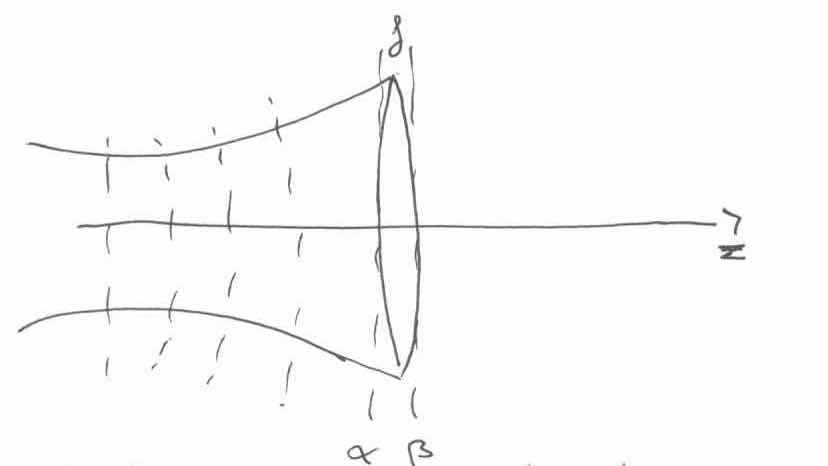
\includegraphics[height=4cm]{images/1}
\end{figure}
Detti $q_\alpha$ e $q_\beta$ i parametri complessi del fascio gaussiano appena prima e appena dopo la lente, per la legge ABCD
\begin{equation*}
q_\beta = \frac{Aq_\alpha + B}{Cq_\alpha + D} \quad \text{con} \quad
\begin{bmatrix}
1	&	0\\
-\frac{1}{f}	&	1
\end{bmatrix}
\end{equation*}
e quindi:
\begin{equation*}
q_\beta = \frac{q_\alpha}{-\frac{1}{f}q_\alpha + 1}
\end{equation*}
Ricordando l'Ansatz: $\frac{1}{q} = \frac{1}{R} -i\frac{\l}{\pi \w^2}$, ho
\begin{equation*}
\frac{1}{R_\beta} -i\frac{\l}{\pi\omega_beta^2} = \frac{1}{R_\alpha} -i\frac{\l}{\pi \omega_\alpha^2} - \frac{1}{f}
\end{equation*}
Uguagliando la parte reale e la parte immaginaria ho infine:
\begin{equation*}
\begin{cases}
\frac{1}{R_\beta} \frac{1}{R_\alpha} - \frac{1}{f}\\
w_\beta = w_\alpha
\end{cases}
\end{equation*}
cioè la lente sottile non modifica lo spot-size del fascio gaussiano mentre ne modifica il suo raggio di curvatura.
\begin{figure}[H]
\centering
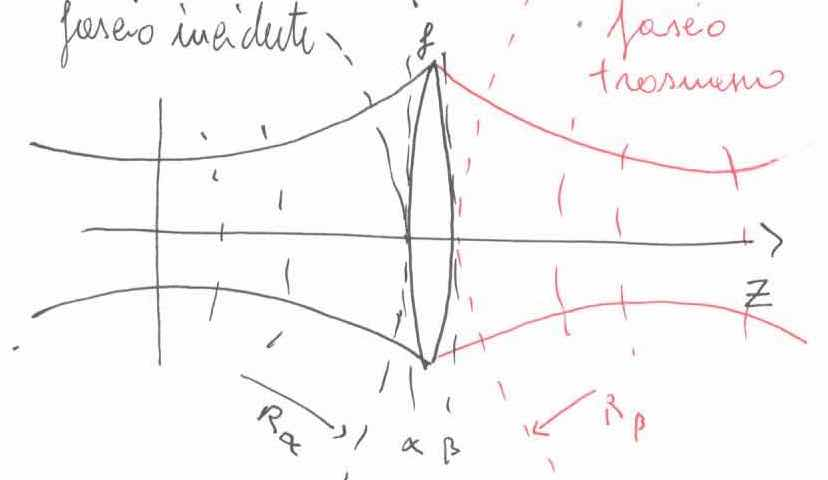
\includegraphics[height=4cm]{images/2}
\end{figure}

2) Focalizzazione di un fascio gaussiano
\begin{figure}[H]
\centering
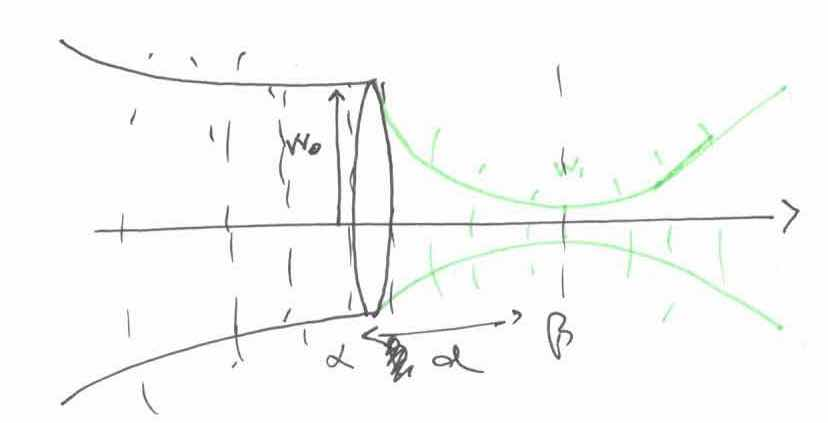
\includegraphics[height=4cm]{images/3}
\end{figure}
Siano $\alpha$ e $\beta$ i piani di figura. Per costruzione $q_\alpha = izR_\alpha =i\frac{\pi w_0^2}{\l}$ e $q_\beta = izR_\beta = i\frac{\pi w_1^2}{\l}$.
Inoltre, per la legge ABCD:
\begin{equation*}
q_\beta = \frac{Aq_\alpha + B}{Cq_\alpha + D} \quad \text{con} \quad
\begin{bmatrix}
1	&	d\\
0	&	1
\end{bmatrix} \begin{bmatrix}
1	&	0\\
-\frac{1}{f}	&	1
\end{bmatrix}
=
\begin{bmatrix}
1-\frac{d}{f}	&	d\\
-\frac{1}{f}	&	1
\end{bmatrix}
\end{equation*}
Pertanto:
\begin{equation*}
iz_{R_\beta} = \frac{iz_{R_\alpha A + B}}{iz_{R\alpha C + D}}\quad -z_{R_\alpha} z_{R_\beta} C +iDz_{R_\beta} = iDz_{R_\alpha} + B
\end{equation*}
Uguagliando la parte reale e immaginaria:
\begin{equation*}
\begin{cases}
z_{R_\alpha} z_{R_\beta} C = -B\\
D z_{R_\beta} = A z_{R\alpha} \rightarrow z_{R_\beta = \frac{A}{D} z_{R\alpha}}
\end{cases}
\end{equation*}
Dalla seconda equazione $z_{R_\beta} = \frac{A}{D} z_{R_\alpha}$, e quindi
\begin{equation*}
z_{R_\alpha}^2 \frac{A}{D} C = -B
\end{equation*}
ovvero:
\begin{equation*}
z_{R_\alpha}^2 \left(1 - \frac{d}{f}\right) \left(-\frac{1}{f}\right) = d
\end{equation*}
quindi:
\begin{align*}
d &= \frac{z_{R_\alpha}^2}{f + \frac{z_{R_\alpha}^2}{f}}\\
&= \frac{f}{1 + \left(\frac{f}{z_{R_\alpha}}\right)^2}
\end{align*}
\begin{equation*}
z_{R_\alpha} = \frac{A}{D}z_{R_\alpha} = 1 - \frac{d}{f} z_{R_\alpha} = \left[ 1 - \frac{1}{1 + \left( \frac{f}{z_{R_\alpha}}\right)}\right] z_{R_\alpha}
\end{equation*}
\begin{equation*}
w_1 = \sqrt{\frac{\left(\frac{f}{z_{R_\alpha}}\right)^2}{1 + \left( \frac{f}{z_{R_\alpha}}\right)^2}} w_0
\end{equation*}
Nel limite $z_R >> f$, ho $d \simeq f$ e $w_1 \simeq w_0 \frac{f}{\frac{\pi w_0^2}{\l}} = \frac{\l}{\pi w_0}f = \theta_d f$ essendo $\theta_d \equiv \frac{\l}{\pi w_0}$ è l'angolo di divergenza del fascio gaussiano incidente.
Interpretazione fisica:
\begin{figure}[H]
\centering
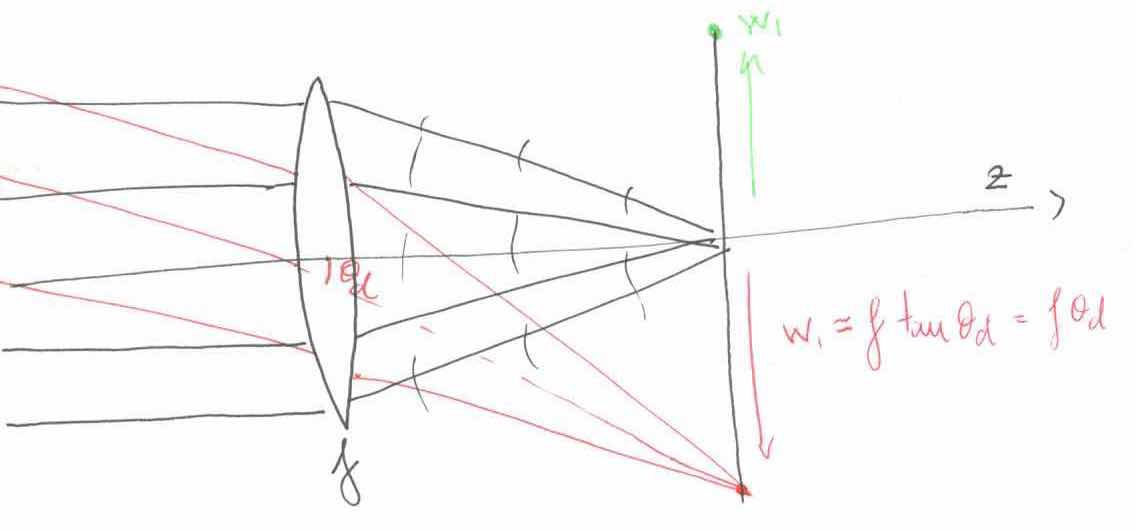
\includegraphics[height=4cm]{images/4}
\end{figure}

3) Legge dei punti coniugati per i fasci gaussiani
\begin{figure}[H]
\centering
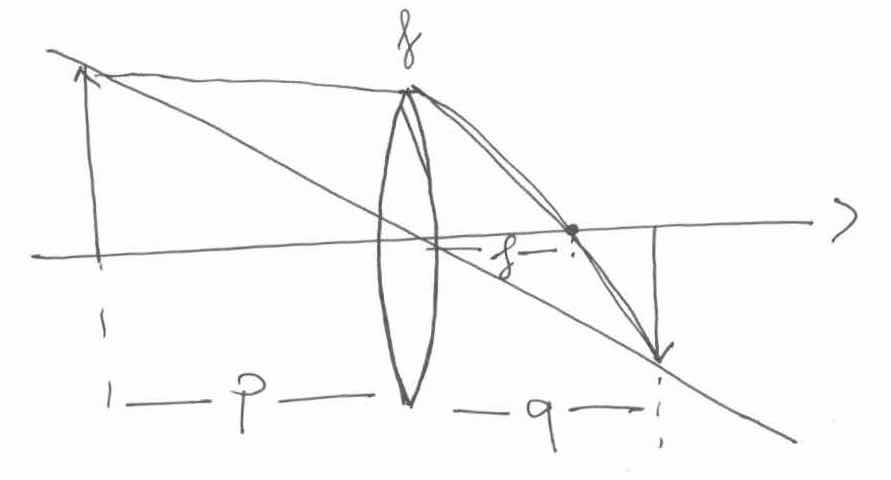
\includegraphics[height=4cm]{images/5}
\end{figure}
Consideriamo $q$ e $w_1$ dato $p$, $w_0$ e $f$ nel seguente problema
\begin{figure}[H]
\centering
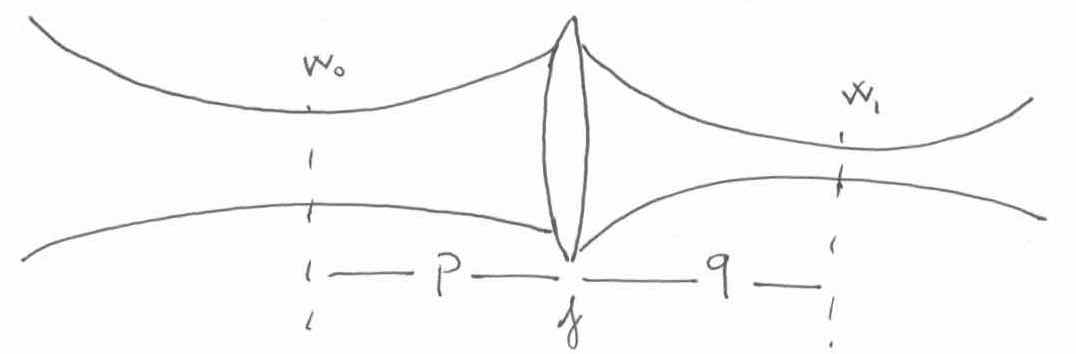
\includegraphics[height=4cm]{images/6}
\end{figure}
Detti $\alpha$ e $\beta$ i piani dei beam waist di figura, per costruzione: $q_\alpha = izR_\alpha =i\frac{\pi w_0^2}{\l}$ e $q_\beta = izR_\beta = i\frac{\pi w_1^2}{\l}$.
Inoltre, per la legge ABCD
\begin{equation*}
q_\beta = \frac{Aq_\alpha + B}{Cq_\alpha + D} \quad \text{con} \quad
\begin{bmatrix}
1	&	q\\
0	&	1
\end{bmatrix} \begin{bmatrix}
1	&	0\\
-\frac{1}{f}	&	1
\end{bmatrix} \begin{bmatrix}
1	&	p\\
0	&	1
\end{bmatrix}
=
\begin{bmatrix}
1-\frac{q}{f}	&	p + q - \frac{pq}{f}\\
-\frac{1}{f}	&	1 - \frac{p}{f}
\end{bmatrix}
\end{equation*}
da cui
\begin{equation*}
iz_{R_\beta} = \frac{iz_{R_\alpha A + B}}{iz_{R\alpha C + D}}\quad -z_{R_\alpha} z_{R_\beta} C +iDz_{R_\beta} = iDz_{R_\alpha} + B
\end{equation*}
uguagliando parte $\Re$ e parte $\Im$ ho
\begin{equation*}
\begin{cases}
-z_{R_\alpha} z_R{\beta} C = B\\
z_{R_\beta} D = A z_{R_\alpha}
\end{cases}
\end{equation*}
Risulta
\begin{equation*}
\frac{1}{q} = \frac{1}{f} - \frac{1}{p} \frac{1}{1 + \frac{z_{R_\alpha}}{p(p-f)}}
\end{equation*}
\begin{equation*}
w_1 = \left|\frac{q}{p}\right| \frac{w_0}{\sqrt{\frac{q}{p} + \left[ 1 + \frac{z_{R_\alpha}}{p(p-f)}\right] \left(	1 - \frac{q}{p}\right)}}
\end{equation*}
%\begin{oss}
\begin{enumerate}
\item Considerando i limite di fascio gaussiano incidente che tende ad un'onda sferica, cioè $z_{R_\alpha} = \frac{\pi w_0^2}{\l} \rightarrow 0$, e $p \neq f$, $p \neq 0$; in tal caso si ha:
\begin{equation*}
\frac{1}{q} \simeq \frac{1}{f} - \frac{1}{p}
\end{equation*}
che è la legge dei punti coniugati dell'ottica geometrica. In tale limite, inoltre
\begin{equation*}
w_1 \simeq \left|\frac{q}{p}\right| w_0
\end{equation*}
che è la legge ordinaria con rapporto d'ingrandimento $M= \left| \frac{q}{p}\right|$.
\item Si consideri il caso $p = f$. In tal caso $q \simeq f$
\end{enumerate}


Tema d'esame 3 Luglio 2009
Si consideri il sistema ottico in figura:
\begin{figure}[H]
\centering
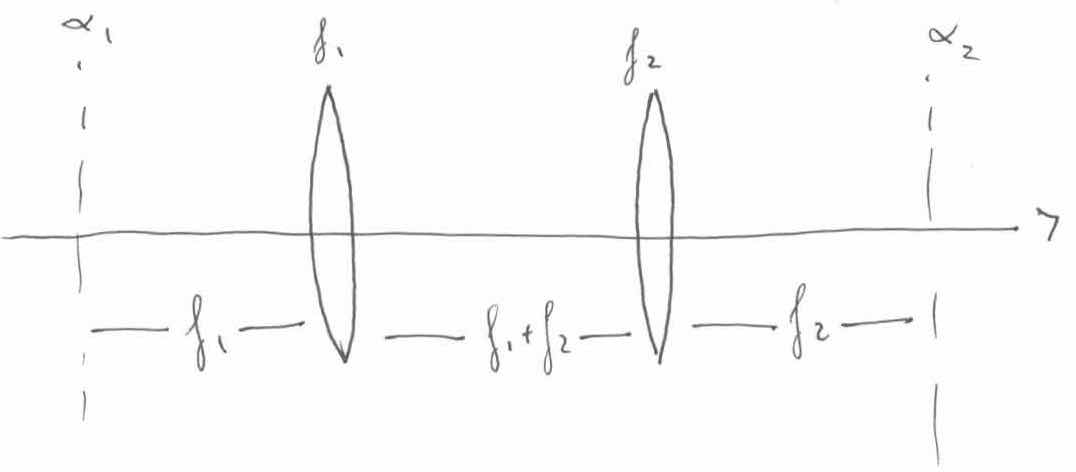
\includegraphics[height=4cm]{images/7}
\end{figure}
1) Calcolare la matrice da $\alpha_1 \rightarrow \alpha_2$:
\begin{equation*}
\begin{bmatrix}
1	&	f_2\\
0	&	1
\end{bmatrix}
\begin{bmatrix}
1	&	0\\
-\frac{1}{f_2}	&	1
\end{bmatrix}
\begin{bmatrix}
1	&	f_1 + f_2\\
0	&	1
\end{bmatrix}
\begin{bmatrix}
1	&	0\\
-\frac{1}{f_1}	&	1
\end{bmatrix}
\begin{bmatrix}
1	&	f_1\\
0	&	1
\end{bmatrix}
=
\begin{bmatrix}
-\frac{f_2}{f_1}	&	0\\
0	&	- \frac{f_1}{f_2}
\end{bmatrix}
\end{equation*}
Usando la legge ABCD si ha che:
\begin{equation*}
q_2 = \frac{Aq_1 + B}{Cq_1 + D}
\end{equation*}
essendo $q_1 + q_2$ i parametri complessi del fascio gaussiano ai piani $\alpha_1$ e $\alpha_2$.
Ricordando l'Ansatz:
$\frac{1}{q_1} = \frac{1}{R_1} -i\frac{\l}{\pi w_1^2}$ e $\frac{1}{q_2} = \frac{1}{R_2} -i\frac{\l}{\pi w_2^2}$ ottengo $q_2 = \frac{A}{D}q_1$, $\frac{1}{q_2} = \frac{D}{A}\frac{1}{q_1}$, ovvero $\frac{1}{R_2} -i\frac{\l}{\pi w_2^2} = \left(\frac{f_1}{f_2}\right)^2 \left[\frac{1}{R_1} - i\frac{\l}{\pi w_1^2}\right]$.
Uguagliando parte reale e parte immaginaria si ha
\begin{equation*}
\begin{cases}
R_2 = \left(\frac{f_2}{f_1}\right)^2 R_1\\
w_2 = \left|\frac{f_1}{f_2}\right|w_1
\end{cases}
\end{equation*}
% Risonatori Ottici
\chapter{Risonatori Ottici}
\graphicspath{{./cap_4/images/}}

\section{Concetti introduttivi}
In un laser il mezzo attivo è posto all'interno di una cavità ottica (risonatore), tipicamente costituito da due o più specchi altamente riflettenti che \textit{intrappolano} la luce al suo interno.
Le cavità ottiche sono cavità aperte. Tali risonatori sostengono delle distribuzioni elettromagnetiche quasi monocromatiche, detti quasi-modi, con frequenze di risonanza $\omega_{n,l,m}$ che dipendono da tre indici:
\begin{description}
\item [n] - indice di modo \textit{longitudinale}; definisce il profilo spaziale del modo nella direzione $z$ dell'asse ottico.
\item [l, m] - indici di modo \textit{trasversale}; definiscono il profilo spaziale del modo nelle direzioni trasversali $x$, $y$ trasversali all'asse ottico.
\end{description}
Esistono due tipologie di risonatori:
\begin{itemize}
\item Risonatori a cavità lineare: Fabry-Perot
\begin{figure}[H]
\centering
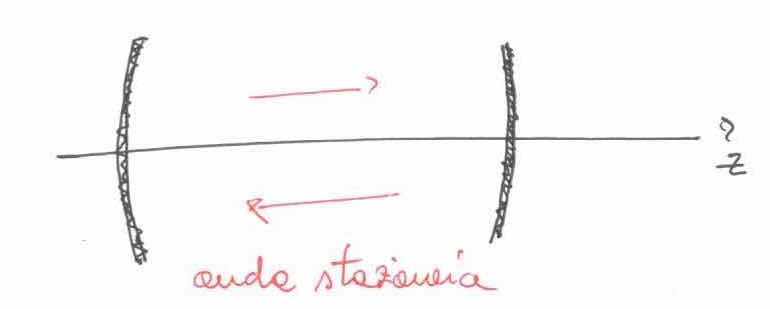
\includegraphics[height=4cm]{images/8}
\end{figure}
\item Risonatori ad anello
\begin{figure}[H]
\centering
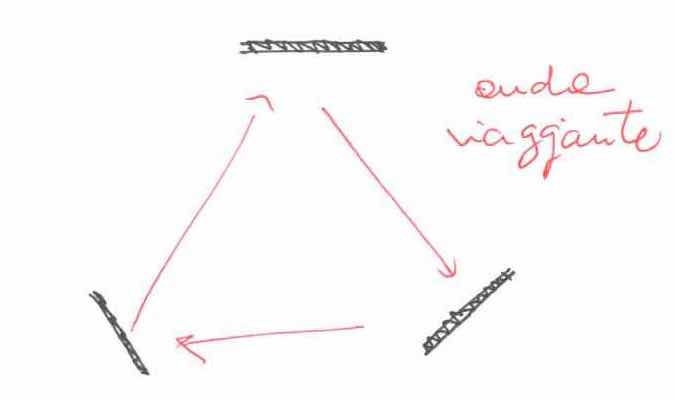
\includegraphics[height=4cm]{images/9}
\end{figure}
\end{itemize}
I risonatori ottici hanno perdite, l'energia può fuoriuscire dal risonatore. Le principali cause di perdite sono:
\begin{description}
\item [Perdite diffrattive] - dovute al fatto che la cavità è aperta.
\item [Perdite di accoppiamento] - dovute alla riflettività $R < 100\%$ dello spettro di uscita.
\item [Perdite di assorbimento/scattering] - dovute agli elementi ottici in cavità.
\end{description}
Le perdite fanno si che le soluzioni d'onda che soddisfano le condizioni al contorno siano della forma:
\begin{equation*}
\*E(x,y,z,t) = \*U_{n,m,l}(x,y,z) \cos(\omega_{n,m,l} t) e^{\frac{t}{2\tau_c}} \quad t \geq 0
\end{equation*}
dove $\omega_{n,m,l}$ è la frequenza di risonanza del quasi-modo, $\*U_{n,m,l}(x,y,z)$ è il profilo di modo, e $\tau_c$ il tempo di vita dei fotoni in cavità del modo ($\tau_c$ in generale dipende dagli indici $n$,$m$,$l$).
Per $\tau_c$ finito, lo spettro di Fourier del campo $\*E$ è una lorentziana centrata in $\omega_{n,m,l}$ con larghezza proporzionale a $\frac{1}{\tau_c}$.
\begin{figure}[H]
\centering
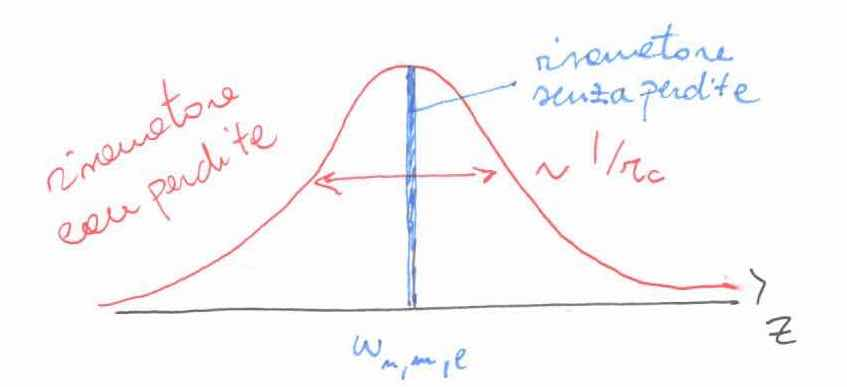
\includegraphics[height=4cm]{images/10}
\end{figure}
\noindent
\begin{example}
Calcolare la frequenza di risonanza di una cavità ottica costituita da due specchi metallici perfettamente riflettenti posti a distanza $L$. Si discutano inoltre le proprietà metalliche dei modi e.m. (onde stazionarie).
\begin{figure}[H]
\centering
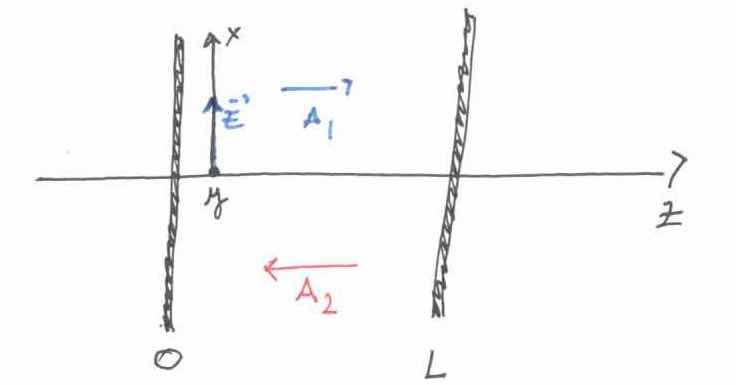
\includegraphics[height=4cm]{images/11}
\end{figure}
\noindent
Cerchiamo una soluzione della forma:
\begin{equation*}
\*E(x,y,z,t) = \frac{1}{2} \left[\underbrace{A_1 e^{i\omega t - ikz}}_\text{onda progressiva} + \underbrace{A_2 e^{i\omega t + ikz}}_\text{onda regressiva} + \,c.c.\right] \widehat{u}_x
\end{equation*}
con $k \equiv \frac{\omega}{c}$.
Le condizioni al contorno, sui due specchi sono:
\begin{equation*}
E_x(z=0,t) \equiv 0 \qquad E_y(z=0,t) \equiv 0
\end{equation*}
che implicano:
\begin{equation*}
\begin{cases}
A_1 e^{i\omega t} + A_2 e^{i\omega t} + c.c. \equiv 0 \qquad \forall t\\
A_1 e^{i\omega t} e^{-ikL} + A_2 e^{i\omega t} e^{ikL} + c.c. \equiv 0 \qquad \forall t
\end{cases}
\end{equation*}
e cioè, necessariamente:
\begin{equation*}
\begin{cases}
A_1 + A_2 = 0\\
A_1 e^{-ikL} + A_2 e^{ikL} = 0
\end{cases}
\end{equation*}
Tale sistema ha soluzione nulla se:
\begin{equation*}
\begin{bmatrix}
1	&	1\\
e^{-ikL}	&	e^{ikL}
\end{bmatrix} = 0
\end{equation*}
cioè $\sin(kL) = 0$ per $kL = n\pi$.
\begin{empheq}[box=\eqbox]{equation*}
\omega_n = kc = \frac{n\pi}{L} c \qquad\text{Frequenza di risonanza con n indice longitudinale}
\end{empheq}
Se $\w=\omega_n$, il campo elettrico vale:
\begin{align*}
\*E(x,y,z,t) &= \frac{1}{2} \left[A_1 e^{i\omega_n t - ik_n z} + A_2 e^{i\omega_n t + ik_n z} + c.c.\right]\\
&= \frac{1}{2} \left[A_1 e^{i\omega_n t} \left(e^{-ik_n z} - e^{ik_n z}\right) + c.c.\right]\\
&= -iA_1 e^i\omega_n t \sin(k_n z) + c.c.
\end{align*}
Posto $E_0 \equiv -2iA_1$ che assumo reale, si ha:
\begin{empheq}[box=\eqbox]{equation*}
E_x(z,t) = E_0 \sin(k_n z) \cos(\omega_n t) \qquad \text{onda stazionaria}
\end{empheq}
%disegno
ci sono $(n+1)$ nodi e $n$ vertici. La condizione di quantizzazione di $k$ si interpreta facilmente pensando alla corda vibrante.
\begin{equation*}
L = n \frac{\l}{2} \quad \text{con} \quad n=1,2,3...
\end{equation*}
Essendo $k = \frac{2\pi}{\l}$ questa condizione equivale a:
\begin{equation*}
L = n\frac{2\pi}{k} \frac{1}{2} = \frac{n\pi}{k} \quad \rightarrow \quad k = \frac{n\pi}{L}
\end{equation*}
\end{example}
\begin{example}
Calcolare i modi e le frequenze di risonanza di una risonatore ad anello a specchi piani in approssimazione di onda piana. Si indichi con $L$ il perimetro dell'anello.
\begin{figure}[H]
\centering
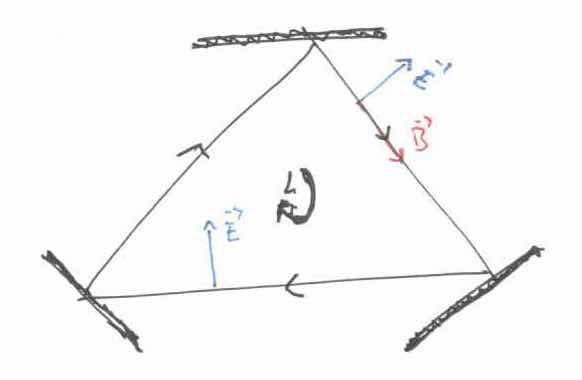
\includegraphics[height=4cm]{images/13}
\end{figure}
\noindent
Detto $z$ l'asse sghembo che descrive il perimetro dell'anello, cerco una soluzione dell'onda viaggiante lungo $z$:
\begin{equation*}
\*E(x,y,z,t) = \frac{1}{2} \left[Ae^{i\omega t -ikz} + c.c. \right] \widehat{u}_x
\end{equation*}
Essendo $z=0$ e $z=L$ i medesimi piani, $E$ in $z=0$ e $z=L$ deve assumere lo stesso valore per ogni $t$, e cioè deve essere soddisfatte le condizioni di autoconsistenza:
\begin{equation*}
E_x(z=0,t) \equiv E_x(z=L, t)
\end{equation*}
e cioè:
\begin{equation*}
A e^{i\omega t} + c.c. \equiv A e^{i\omega t - ikL} + c.c. \quad \forall t
\end{equation*}
che implica necessariamente:
\begin{equation*}
e^{-ikL} = 1
\end{equation*}
cioè:
\begin{equation*}
kL = 2n\pi \qquad \begin{cases}
k = k_n = \frac{2n\pi}{L}\\
\omega = \omega_n = \frac{2\pi c}{L} n
\end{cases}
\end{equation*}
$\nu_n = \frac{cn}{L}$ frequenza di risonanza del risonatore ad anello.

\begin{os}
La frequenza di risonanza longitudinale di un
Fabry-Perot di lunghezza $L$ è $\D\omega = \frac{\pi c}{L}$.
\end{os}
\begin{figure}[H]
\centering
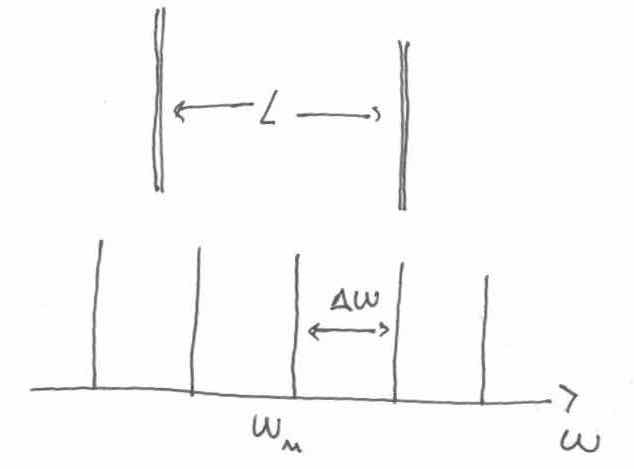
\includegraphics[height=4cm]{images/14}
\end{figure}
\noindent
Per una cavità ad anello $\D\omega = \frac{2\pi c}{L}$.
\begin{figure}[H]
\centering
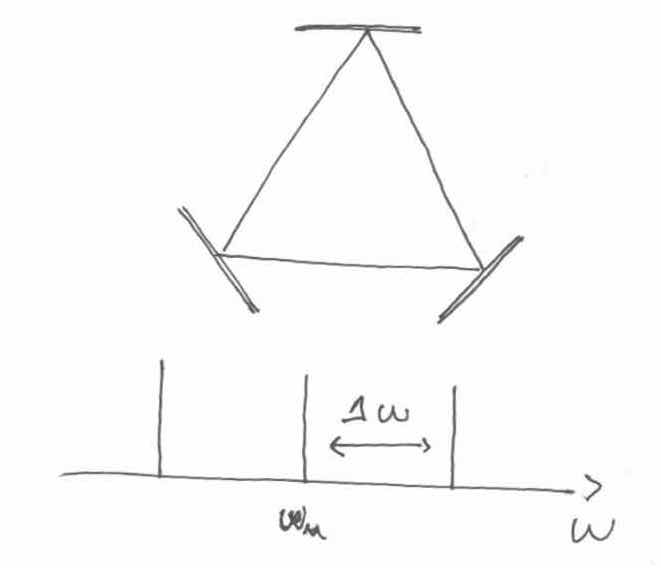
\includegraphics[height=4cm]{images/15}
\end{figure}
\end{example}

\begin{example}
Calcolare il numero di modi che cadono sotto la riga di guadagno di un mezzo attivo laser, con larghezza di riga $\D\nu_0$, nei seguenti casi:
\begin{enumerate}
\item cavità cilindrica chiusa di lunghezza $L$ e raggio $a$ con pareti metalliche perfettamente riflettenti
\item cavità aperta costituita dalla precedente rimuovendo la superficie laterale del cilindro.
\end{enumerate}
\begin{figure}[H]
\centering
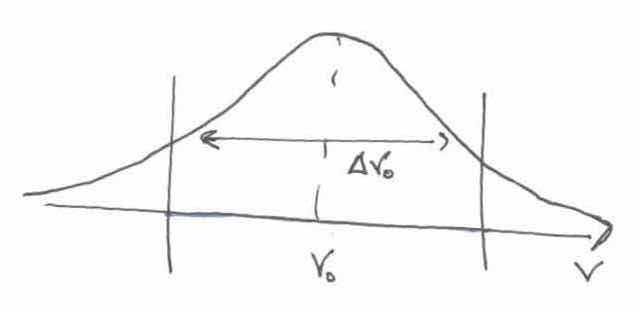
\includegraphics[height=4cm]{images/16.jpg}
\end{figure}
\begin{enumerate}
\item È noto che, per una cavità chiusa di volume $V$, la densità spettrale dei modi e.m. della cavità vale:
\begin{equation*}
\rho(\nu) = \frac{8\pi \nu^2 V}{c^3}
\end{equation*}
cioè $\rho(\nu) d\nu$ è il numero di modi con frequenza compresa tra $\nu$ e $\nu + d\nu$.
Quindi:
\begin{equation*}
N^{(closed)} = \rho(\nu_0) \D \nu_0 = \frac{8\pi \nu_0^2 V}{c^3} \D\nu_0
\end{equation*}
\item In questo caso i modi con basse perdite sono solo onde che si propagano lungo l'asse $z$. Le figure di tali modi sono equispaziati di:
\begin{equation*}
\D\nu = \frac{\D\omega}{2\pi} = \frac{c}{2L}
\end{equation*}
\begin{equation*}
N^{(open)} = \left\lfloor \frac{\D \nu_0}{\D \nu} \right\rfloor = \frac{\D \nu_0}{\frac{c}{2L}}
\end{equation*}
Calcolo il rapporto tra il numero di modi nei due casi:
\begin{equation*}
\frac{N^{(closed)}}{N^{(open)}} = \frac{\frac{8\pi \nu_0^2}{c^3} \D \nu_0 \pi a^2 L}{\frac{\D \nu_0}{\frac{c}{2L}}} = ... = \left( \frac{2\pi a}{\l_0} \right)^2
\end{equation*}
\end{enumerate}

\begin{exercise}
Si consideri un laser $HeNe$ con i seguenti parametri costruttivi:\\
$L = 50 cm$ $\l_0 = 633 nm$ $2a = 3 mm$ $\D\nu_0 = 1.7GHz$\\
Utilizzando quanto visto in precedenza si ha:
\begin{equation*}
N^{(open)} \simeq 6
\end{equation*}
\begin{equation*}
\frac{N^{(closed)}}{N^{(open)}} = 1.2 \cdot 10^9
\end{equation*}
Con una cavità chiusa ci sarebbero una quantità enorme di modi che verrebbero amplificati risultando in una sorgente non monocromatica. Viceversa, nel caso di cavità aperta i modi sono solamente 6. Ecco spiegato perché i laser sono costituiti da cavità aperte e non chiuse.
\end{exercise}
\end{example}

\section{Teoria geometrica dei risonatori ottici: Teorema di stabilità}
Considero un risonatore a cavità lineare costituita da due specchi sferici terminali, di raggi di curvatura $R_1$ e $R_2$, posti a distanza $L$. Tra i due specchi, in generale, possono esservi altri elementi ottici (lenti). L'asse ottico $z$ del risonatore è la retta che congiunge i centri degli specchi.
%disegno
Preso un piano $\gamma$ perpendicolare a $z$ interno al risonatore, studiamo la propagazione di un raggio parassiale che rimbalza avanti e indietro tra i due specchi.
Sia $(r_0,r_0'), (r_1,r_1'), \dots, (r_n,r_n'), \dots$ i parametri parassiali del raggio, quando attraverso il piano $\gamma$ da sinistra a destra, all'n-esimo round-trip.

Definizione
Il risonatore si dice stabile secondo l'ottica geometrica se, fissati $(r_0,r_0')$ ad arbitrio, $r_n$ e $r_n'$ non divergono se $n\rightarrow\infty$. Cioè, il risonatore è stabile se è in grado di intrappolare i raggi che rimbalzano tra i due specchi.

Si noti che la propagazione di un raggio luminoso tra i due specchi del risonatore è equivalente alla propagazione di un raggio nella lensguide così costruita.
%disegno
La matrice trasmissione di uno specchio in riflessione è uguale a quella di una lente in trasmissione se $f = \frac{R}{2}$.\\
Specchio
\begin{equation*}
\begin{bmatrix}
1	&	0\\
-\frac{2}{R}	&	1
\end{bmatrix}
\end{equation*}
Lente
\begin{equation*}
\begin{bmatrix}
1	&	0\\
-\frac{1}{f}	&	1
\end{bmatrix}
\end{equation*}
Vale il fondamentale teorema di stabilità: sia la matrice ABCD la matrice round-trip del risonatore rispetto al piano $\gamma$, cioè la matrice a raggi del piano $z=0$ al piano $z=2L$ nella lensguide equivalente. Allora il risonatore è stabile secondo l'ottica geometrica se è soddisfatta la seguente
\begin{equation*}
\left| \frac{A+D}{2} \right| < 1
\end{equation*}
Infatti, per definizione di matrice ABCD, si ha:
\begin{equation*}
\begin{bmatrix}
r_1\\
r_1'
\end{bmatrix} = 
\begin{bmatrix}
A	&	B\\
C	&	D
\end{bmatrix}
\begin{bmatrix}
r_0\\
r_0'
\end{bmatrix},
\begin{bmatrix}
r_2\\
r_2'
\end{bmatrix} = 
\begin{bmatrix}
A	&	B\\
C	&	D
\end{bmatrix}
\begin{bmatrix}
r_1\\
r_1'
\end{bmatrix} =
\begin{bmatrix}
A	&	B\\
C	&	D
\end{bmatrix}^2
\begin{bmatrix}
r_0\\
r_0'
\end{bmatrix},\dots
\begin{bmatrix}
r_n\\
r_n'
\end{bmatrix}
=\begin{bmatrix}
r_1\\
r_1'
\end{bmatrix} = 
\begin{bmatrix}
A	&	B\\
C	&	D
\end{bmatrix}^n
\begin{bmatrix}
r_0\\
r_0'
\end{bmatrix}
\end{equation*}
Dalla definizione di stabilità, il risonatore è stabile se:
\begin{equation*}
|r_n| < \infty, \qquad |r_n'| < \infty
\end{equation*}
per $n\rightarrow \infty$, qualunque sia $(r_0, r_0')$.
Posto $M \equiv \begin{bmatrix}
A	&	B\\
C	&	D
\end{bmatrix}$, detta $\begin{bmatrix}
\l_1	&	0\\
0	&	\l_2
\end{bmatrix}$ e $T$ la matrice diagonale $\Lambda$ degli autovalori $(\l_1,\l_2)$ di $M$ e dei corrispondenti autovettori
\begin{equation*}
MT = T\Lambda
\end{equation*}
se $T$ è invertibile, ho:
\begin{equation*}
M = T\Lambda T^{-1}
\end{equation*}



e poiché
\begin{equation*}
\Lambda^n = \begin{bmatrix}
\l_1	&	0\\
0	&	\l_2
\end{bmatrix}^n = \begin{bmatrix}
\l_1^n	&	0\\
0	&	\l_2^n
\end{bmatrix}
\end{equation*}
si ha
\begin{equation*}
\begin{bmatrix}
r_n\\
r_n'
\end{bmatrix} =
T\begin{bmatrix}
\l_1^n	&	0\\
0	&	\l_2^n
\end{bmatrix}
T^{-1}\begin{bmatrix}
r_0\\
r_0'
\end{bmatrix}
\end{equation*}
Per $n\rightarrow\infty$, $|r_n|$ e $r_n'$ sono limitati se e solo se:
\begin{equation*}
|\l_1| \leq 1, \qquad 
\end{equation*}
Calcolo $\l_1$ e $\l_2$
\begin{equation*}
\begin{bmatrix}
\l_1	&	0\\
0	&	\l_2
\end{bmatrix} = 0
\end{equation*}
\begin{align*}
&(\l-A)(\l-D)-BC = 0\\
&\l^2-(A+D)\l+\underbrace{AD-BC}_\text{det M = 1} = 0
\end{align*}
Introdotto l'angolo $\theta$ così definito:
\begin{equation*}
\cos \theta \equiv \frac{A+D}{2}
\end{equation*}
\begin{equation*}
\l^2 - 2\cos\theta\l + 1 = 0, \quad \l_{1,2} = \cos\theta \pm \sqrt{\cos^2\theta -1} = \cos\theta \pm i\sin\theta = e^{\pm i\theta}
\end{equation*}
cioè:
\begin{equation*}
\l_{1,2} = e^{\pm i\theta}
\end{equation*}
Distinguo tre casi:
\begin{enumerate}
\item $\left|\frac{A+D}{2}\right|<1$, $\theta$ reale, $|\l_1|=|\l_2|=1$ e il risonatore è stabile.
\item $\frac{A+D}{2}>1$, $\theta = i\psi$ con $cosh \psi=\frac{A+D}{2}$, $psi$ reale. Per cui $|\l_1|= e^{i\theta}=e^{-\psi}$, $\l_2=e^\psi$ uno dei due autovalori ha modulo maggiore di uno quindi il risonatore è instabile.
\item $\frac{A+D}{2}<-1$, posto $\theta=i\psi+\pi$ ho $cosh \psi=-\frac{A+D}{2} = \left|\frac{A+D}{2}\right|$ cioè $psi$ reale. In tal caso: $\l_{1,2}= e^{\pm i\theta}=e^{\pm i\theta \mp \psi} = -e^{\mp\psi}$. Ancora, uno dei due autovalori ha modulo maggiore di uno quindi il risonatore è instabile.
\end{enumerate}

Esempio notevole: risonatore a die specchi sferici
%disegno
Considero due specchi sferici di raggio di curvatura $R_1$ e $R_2$ a distanza $L$ fra i quali c'è il vuoto. Scelto $\gamma$ come in figura, la lensguide equivalente è:
%disegno
La matrice $M$ di round trip rispetto a $\gamma$ vale:
\begin{equation*}
M = \begin{bmatrix}
1	&	0\\
-\frac{2}{R_1}	&	1
\end{bmatrix}
\begin{bmatrix}
1	&	L\\
0	&	1
\end{bmatrix}
\begin{bmatrix}
1	&	0\\
-\frac{2}{R_2}	&	1
\end{bmatrix}
\begin{bmatrix}
1	&	L\\
0	&	1
\end{bmatrix} = \dots
\end{equation*}
da cui:
\begin{equation*}
\frac{A+D}{2} = 2(1-\frac{L}{R-1})(1-\frac{L}{R_2}) - 1
\end{equation*}
Introdotti i parametri $g_1, g_2$ del risonatore così definiti:
\begin{equation*}
g_1 \equiv 1-\frac{L}{R_1}, \quad g_2 \equiv 1-\frac{L}{R_2}
\end{equation*}
la condizione di stabilità diventa
\begin{equation*}
-1 < 2g_1 g_2 -1 <1
\end{equation*}
cioè:
\begin{equation*}
0 < g_1g_2 < 1 \qquad \text{Condizione di stabilità (per questo caso)}
\end{equation*}
Diagramma di stabilità del piano $(g_1,g_2)$
%disegno
Caso notevole:
risonatori simmetrici ha $R_1=R_2=R$, da cui $g_1=g_2=1-\frac{L}{R}$
Si noti che esistono 3 risonatori simmetrici al limite della stabilità:
\begin{enumerate}
\item $g_1=g_2=1$ cioè $R=0$: Risonatore piano-piano
%disegno
Non è stabile
\item $g_1=g_2=0$ cioè $R=L$: Risonatore confocale
%disegno
è stabile e ogni raggio ritorna su se stesso dopo due round trip
\item $g_1=g_2 = -1$ cioè $L=2R$: Risonatore concentrico
%disegno
È instabile
\end{enumerate}
Osservazione
La teoria svolta, fino al teorema di stabilità incluso, (escludere esempio notevole) vale




\section{Teoria ondulatoria dei risonatori:  modi e frequenze di risonanza}
Considero un risonatore a cavità lineare, costituito da due specchi terminali di raggi di curvatura $R_1$ e $R_2$ posti a distanza $L$, fra gli specchi possono essere interposti altri elementi (lenti). Supponiamo che:
\begin{enumerate}
\item Gli specchi sono infinitamente estesi (trascuro gli effetti di bordo e perdite diffrattive)
\item  Suppongo gli specchi riflettenti al 100\% (i quasi-modi sono modi)
\item Considero onde e.m. parassiali in approssimazione scalare (modi quasi TEM). La propagazione di un campo e.m. intrappolato fra i due specchi, rappresentabile dalla sovrapposizione o interferenza di due onde parassiali contropropagantesi può essere descritta in maniere sostanzialmente equivalente alla propagazione di un'onda viaggiante nella lens guide equivalente.
%disegno
Tracciamo la lens guide (unfolding):
%disegno
\end{enumerate}
Detto $\*E(x,y,z,t) = \frac{1}{2} [u(x,y,z) e^{i\omega t-ikz} + c.c.] \*u_x$ il campo che si propaga nella lensguide ho un inviluppo $u(x,y,z)$ che in funzione di $z$ varia in accordo dell'integrale generalizzato di KHF. Nel problema originale, i percorsi $z=0$ e $z=2L$ sono il medesimo piano $\gamma$; pertanto, per monodromia, deve aversi:
\begin{equation*}
E_x(x,y,0,t) \equiv E_x(x,y,2L,t) \qquad \forall t
\end{equation*}
condizione di autoconsistenza

ovvero:
\begin{equation*}
u(x,y,0) = u(x,y,2L) e^{-2ikL}
\end{equation*}
Del resto, detta ABCD la matrice di roundtrip del risonatore rispetto al piano $\gamma$, si ha:
\begin{equation}
u(x,y,2L) = \iintinf u(x_1,y_1,0)K(x,x_1y,y_1)dx_1dy_1
\end{equation}
dove $K \equiv \frac{i}{\l B} e^{-\frac{ik}{2B} [A(x_1^2 + y_1^2) + D(x^2 + y^2) - 2xx_1 - 2yy_1]}$ è il nucleo (kernel) dell'integrale generalizzato di KHF. Sinteticamente scrivo:
\begin{equation*}
u(x,y,2L) = \widehat{K} u(x,y,0)
\end{equation*}
dove $\widehat{K}$ è l'operatore integrale di KHF.
La condizione di autoconsistenza è quindi:
\begin{equation*}
u(x,y,0) = e^{-2ikL} \widehat{K} u(x,y,0)
\end{equation*}
cioè:
\begin{empheq}[box=\eqbox]{equation*}\label{eq: }
\widehat{K}u(x,y,0) = \sigma u(x,y,0)
\end{empheq}
con $\sigma \equiv e^{2ikL}$.
Ciò significa che le eventuali soluzioni monocromatiche parassiali a frequenza $\w$ che soddisfano il problema e.m. tra i due specchi e le condizioni al contorno imposte dagli specchi sono le autofunzioni dell'operatore $\widetilde{K}$ con autovalori $\sigma = e^{2ikL}$ (eq.di Fredholm). Cerchiamo una soluzione dell'equazione agli autovalori della forma:
\begin{equation*}
u(x,y,0) = u_0 H_l\left(\frac{\sqrt{2}x}{w_1}\right)H_m\left(\frac{\sqrt{2}y}{w_1}\right) e^{-i\frac{k(x^2 + y^2)}{2q_1}}
\end{equation*}
cioè con distribuzione di Gauss-Hermite, dove $\Im{\frac{1}{q_1}}<0$. Sappiamo che:
\begin{equation*}
\widehat{K}u(x,y,0) = \frac{u_0}{\left(A+\frac{B}{q_1}\right)^{1+l+m}} H_l\left(\frac{\sqrt{2}x}{w}\right)H_m\left(\frac{\sqrt{2}y}{w}\right) e^{-i\frac{k(x^2 + y^2)}{2q}}
\end{equation*}
dove $q$ è dato dalla legge ABCD $q = \frac{Aq_1 + B}{Cq_1 + D}$
Imponiamo la \eqref{} \begin{equation*}
\widehat{K}u(x,y,0) = \sigma u(x,y,0)
\end{equation*}
Ciò implica:
\begin{equation*}
\begin{cases}
q=q_1\\
\sigma = \frac{1}{\left(A + \frac{B}{q_1}\right)^{1+l+m}}
\end{cases}
\end{equation*}
Studiamo le equazioni:
\begin{enumerate}
\item $q=q_1$ e cioè $q_1 = \frac{Aq_1 + B}{Cq_1 + D}$ ovvero:
\begin{equation*}
Aq + B = Cq^2 + Dq
\end{equation*}
o anche
\begin{equation*}
\frac{A}{q} + \frac{B}{q^2} = c +\frac{D}{q}, \quad B\left(\frac{1}{q}\right)^2 + (A-D)\left(\frac{1}{q}\right) -C = 0
\end{equation*}
Le soluzioni sono:
\begin{equation*}
\left(\frac{1}{q}\right)_{\pm} = -\frac{A-D}{2B} \pm \frac{1}{B}\sqrt{\left(\frac{A-D}{2}\right)^2 + BC}
\end{equation*}
Osservando che:
\begin{align*}
\left(\frac{A-D}{2}\right)^2 + BC &= \frac{A^2 +D^2 -2AD + 4BC}{4}\\
&= \frac{A^2 + D^2 - 2AD + 4(AD-1)}{4}\\
&= \frac{(A+D)^2 -4}{4}\\
&= \cos^2\theta -1 
\end{align*}
ricordando l'Ansatz $\cos\theta \equiv \frac{A+D}{2}$.
Pertanto:
\begin{equation*}
\left(\frac{1}{q}\right)_{\pm} = - \frac{A-D}{2B} \pm \frac{i\sin\theta}{B}
\end{equation*}
Le soluzioni accettabili sono quelle $Im{\frac{1}{q}}<0$ per confinamento. Osserviamo che, se $\left|\frac{A+D}{2}\right|>1$, $\theta = i\psi$ oppure $\theta=i\psi +\pi$ con $\psi$ reale e quindi $i\sin\theta$ reale. Per cui quando $Im{\frac{1}{q}}_\pm = 0$. Non ci sono soluzioni accettabili.
Se il risonatore è instabile secondo l'ottica geometrica (vedi. Th di stabilità) l'eq. agli autovalori di Fredholm non ha soluzioni in $L^2$: non ci sono modi e.m. confinati.
Se invece $\left|\frac{A+D}{2}\right|<1$, $\sin\theta$ è reale, $\Im{\frac{1}{q}_\pm}= \pm\frac{\sin\theta}{B}$ e quindi esiste una e una sola soluzione accettabile.
\item Seconda equazione:
\begin{align*}
e^{2ikL} &= \frac{1}{\left(A + \frac{B}{q_1}\right)^{1+l+m}}\\
&= \frac{1}{\left(A + \frac{A-D}{2}\pm i\sin\theta\right)^{1+l+m}}\\
&= \frac{1}{\left(\cos \theta \pm \sin \theta\right)^{1+l+m}}\\
&= \frac{1}{e^{\pm i\theta(i+l+m)}}
\end{align*}
cioè:
$e^{2ikL} = e^{\mp i\theta(1+l+m)}$ che implica $2kL = \mp \theta(1+l+m) + 2\pi n$ con $n$ intero. $k = \frac{\pi n}{L} \mp \frac{\theta}{2L}(1+l+m)$. $\nu = \frac{\omega}{2\pi} = \frac{kc}{2\pi} = \frac{c}{2L} \left[n \mp \frac{\theta}{2\pi}(1+l+m)\right]$
cioè:
\begin{equation*}
\nu_{n,l,m} = \frac{c}{2L} \left[n \mp \frac{\theta}{2\pi}(1+l+m)\right]
\end{equation*}
frequenza di risonanza

$\nu$ dipende da tre indici:
\begin{description}
\item [n] indice longitudinale
\item [l,m] indici trasversali
\end{description}

\end{enumerate}

Esempio: frequenza di risonanza del risonatore confocale

\begin{equation*}
\nu_{n,l,m} = \frac{c}{2L} \left[n \mp \frac{\theta}{2\pi}(1+l+m)\right]
\end{equation*}
con $\cos\theta = \frac{A+D}{2}$.
Calcolo matrice ABCD per confocale.
%disegno
%disegno
\begin{equation*}
M = \begin{bmatrix}
A	&	B\\
C	&	D
\end{bmatrix}
=\begin{bmatrix}
1	&	0\\
-\frac{2}{R}	&	1
\end{bmatrix}\begin{bmatrix}
1	&	R\\
0	&	1
\end{bmatrix}\begin{bmatrix}
1	&	0\\
-\frac{2}{R}	&	1
\end{bmatrix}\begin{bmatrix}
1	&	R\\
0	&	1
\end{bmatrix}=\begin{bmatrix}
-1	&	0\\
0	&	-1
\end{bmatrix}=-I
\end{equation*}
Si noti che $M^2 = I$: ciò significa che, in un confocale, dopo due round-trip ogni distribuzione di campo e.m. ritorna ad essere uguale a se stessa.
Per il confocale, o vicino alla confocalità, il valore di $\theta$ vale:
\begin{equation*}
\cos\theta = \frac{A+D}{2}\simeq -1
\end{equation*}
cioè $\theta=\pi$. Quindi:
\begin{equation*}
\nu_{n,l,m} = \frac{c}{2L} \left[n + \frac{1}{2}(1+l+m)\right] = \frac{c}{4L} \left[2n + (1+l+m)\right]
\end{equation*}
%disegno
Si noti che al variare di $n,l,m$, $\nu_{n,l,m}$ descrive un pettine di frequenze con i centri equispaziati di $\frac{c}{4L}$ (v. figura). Ogni frequenza di risonanza è infinite volte degenere.
Osservazione: si noti che se applico la condizione di autoconsistenza nel confocale e cioè la prima eq di ieri: $q = \frac{Aq_1 + B}{Cq_1 + D}$
essendo $A=D=-1$, $B=C=0$ si ha: $q=q$ identità.

Esercizio 1
i) Detta ABCD la matrice di round trip rispetto a $\gamma$ il parametro $q$ del modo $TEM_{00}$ del risonatore in $\gamma$ soddisfa la condizione di autoconsistenza $q = \frac{Aq_1 + B}{Cq_1 + D}$ ovvero $\left(B\frac{1}{q}\right)^2 + (A-D)\frac{1}{q} - C = 0$. Su $\gamma$, il raggio di curvatura $R_\gamma$ e lo spot size $w_\gamma$ del modo $TEM_{00}$ sono dati dall'Ansatz:
\begin{equation*}
\frac{1}{q} = \frac{1}{R_\gamma} -i\frac{\l}{\pi w_\gamma^2}
\end{equation*}
Su $\gamma$ il modo ha un beam waist se $R_\gamma=\infty$, cioè $q$ puramente immaginario. Essendo:
\begin{equation*}
\frac{1}{q}_\pm = -\frac{A-D}{2B} \pm i\frac{\sin\theta}{B}
\end{equation*}
per risonatore stabile $\theta$ reale, quindi $\Re{\frac{1}{q}}=0$ se e solo se $A=D$.\\
ii) Dimostrare che la semi traccia della matrice ABCD non dipende dal piano $\gamma$.\\
%disegno
Siano $\gamma$ e $\beta$ due piani interni al risonatore. Facciamo la lensguide rispetto a $\gamma$:
%disegno
Dette $M_\gamma$ e $M_\beta$ le matrici di round trip rispetto ai piani $\gamma$ e $\beta$ si ha evidentemente:
\begin{equation*}
M_\gamma = M_2M_1 \qquad M_\beta = M_1M_2
\end{equation*}
Essendo il prodotto di matrici non commutativo in generale $M_\beta \neq M_\gamma$.\\
Per la proprietà di invarianza della traccia del prodotto di matrici per permutazioni cicliche, ad es.
\begin{equation*}
Tr(ABC) = Tr(CAB) = Tr(BCA)
\end{equation*}
si ha $Tr(M_\gamma) = Tr(M_\beta)$.\\
\\
Esercizio 2
Laser Ti:sapphire ($\l=780nm$)
perimetro $L$
$f = 2cm$\\
i) Calcolare $L=L_{max}$ per cui $L<L_{max}$ il risonatore è stabile.
Scelto il piano $\gamma$ come in figura, la matrice ABCD di transito nell'anello da $\gamma\rightarrow\gamma$ vale:
\begin{equation*}
\begin{bmatrix}
A	&	B\\
C	&	D
\end{bmatrix}
=\begin{bmatrix}
1	&	\frac{L}{2}\\
0	&	1
\end{bmatrix}\begin{bmatrix}
1	&	0\\
-\frac{1}{f}	&	1
\end{bmatrix}\begin{bmatrix}
1	&	\frac{L}{2}\\
0	&	1
\end{bmatrix}=\begin{bmatrix}
1-\frac{L}2f{}	&	L-\frac{L^2}{4f}\\
-\frac{1}{f}	&	1-\frac{L}{2f}
\end{bmatrix}
\end{equation*}
Per il th di stabilità, il risonatore è stabile:
\begin{equation*}
-1 < \frac{A+D}{2} < 1
\end{equation*}
cioè:
\begin{equation*}
-1 < 1-\frac{L}{2f} < 1, \quad \begin{cases}
1 - \frac{L}{2f} < 1 \rightarrow \frac{L}{2f} > 0 \text{ovvia}\\
1-\frac{L}{2f} > -1 \rightarrow \frac{L}{2f} < 2 \rightarrow L_{max} =4f
\end{cases}
\end{equation*}
ii) Calcolare la posizione del punto di vita del fascio dentro l'anello, la dimensione di macchia e la dimensione di macchia della lente nel caso in cui $L_{max} = \frac{L}{2} = 2f$.
Il parametro $q$ del modo $TEM_00$ al piano $\gamma$ si ottiene dalla condizione di autoconsistenza: $q = \frac{Aq_1 + B}{Cq_1 + D}$
\begin{equation*}
Cq^2 + Dq = Aq + B, \quad q^2=\frac{B}{C} = \frac{L - \frac{L^2}{4f}}{-\frac{1}{f}} = \frac{2f - f}{-\frac{1}{f}}
\end{equation*}
cioè $q^2 = -f^2$, ovvero $q = if$.
Essendo $q$ puramente immaginario su $\gamma$, $R_\gamma=\infty$ cioè su $\gamma$ il fronte di fase è piano e il modo $TEM_{00}$ ha il suo beam waist. Quanto vale $w_0$ nel punto di vita? Ricordo che, per fascio gaussiano in propagazione libera con beam waist in $z=0$, $q(z) = z +iz_R$ dove $z_R \equiv \frac{\pi w_0^2}{\l}$. Pertanto:
\begin{equation*}
\frac{\pi w_0^2}{\l} = f, w_0 = \sqrt{\frac{\l f}{\pi}} = 705 \mu m
\end{equation*}
Per calcolare $w_\beta$ osservo che dal beam waist sul piano $\gamma$ il fascio $TEM_{00}$ si propaga in propagazione libera fino a $\beta$. Pertanto:
\begin{equation*}
w_\beta = w_\gamma \sqrt{1+ \left(\frac{\frac{L}{2}}{f}\right)^2} = \sqrt{2}w_\gamma
\end{equation*}
cioè:
\begin{equation*}
w_\beta = \sqrt{2}w_\gamma = \sqrt{\frac{2\l f}{\pi}} \simeq 997 \mu m
\end{equation*}







\section{Risonatori con perdite: $\tau_c$ e fattore di qualità Q di un risonatore}
Considero cavità ottica lineare con specchi di riflettività $R_1$ e $R_2$. Preso u piano $\gamma$ interno al risonatore e detta $I(T)$ l'intensità al tempo $t$ dell'onda progressiva al piano $\gamma$ e al tempo $t$, si ha:
\begin{equation*}
I(t+T_R) = R_1R_2 (1-T_1)^2 I(t)
\end{equation*}
dove $T_R \equiv \frac{2L_c}{c_0}$ è il tempo di round-trip della luce nel risonatore, $L_c$ lunghezza ottica $L_c = \int_0^L n(z) dz$ $T_1$ trasmissione fittizia che tiene conto delle perdite interne per singolo transitorio.
Cerco una soluzione dell'equazione alle differenze con l'Ansatz:
\begin{equation*}
I(t) = I(0) e^{-\frac{t}{\tau_c}}
\end{equation*}
con $\tau_c$ costante di tempo (tempo di vita dei fotoni in cavità) da determinarsi. Sostituisco l'Ansatz:
\begin{equation*}
I(0) e^{-\frac{t+T_R}{\tau_c}} = R_1 R_2 (1 + T_1)^2 I(0)e^{-\frac{t}{\tau_c}}
\end{equation*}
e cioè
\begin{equation*}
e^{-\frac{T_R}{\tau_c}} = R_1 R_2 (1 + T_1)^2
\end{equation*}
da cui
\begin{equation*}
\frac{T_R}{\tau_c} = -\ln R_1 - \ln R_2 - 2 \ln(i-T_i)
\end{equation*}
Introdotte le cosiddette perdite logaritmiche (per singolo passaggio) del risonatore:
\begin{equation*}
\gamma \equiv \frac{\gamma_1 + \gamma_2}{2} + \gamma_i
\end{equation*}
con \begin{align*}
&\gamma_1 \equiv -\ln R_1\\
&\gamma_2 \equiv -\ln R_2\\
&\gamma_i \equiv -\ln (1-T_r)
\end{align*}
si ha $\frac{T_R}{\tau_c} = 2 \gamma$ ovvero $\tau_c = \frac{T_R}{2\gamma} = \frac{L_c}{c_0 \gamma}$ tempo di vita dei fotoni in cavità.
\\
Il campo elettrico in un punto del risonatore, decade, a causa delle perdite, con la relazione
\begin{equation*}
E(t) = E_0 \cos(\omega_c t) e^{-\frac{t}{2\tau_c}}
\end{equation*}
dove $\omega_c = \omega_{n,m,l}$ è una frequenza di risonanza calcolata nel caso di risonatori senza perdite. Lo spettro di potenza di $E(t)$ vale
\begin{equation*}
\tilde{E(\w)} \equiv \left| \int_0^\infty E_0 \cos(\omega_c t) e^{-\frac{t}{2\tau_c}} e^{i\omega t}
dt \right|^2 = \left( \frac{E_0}{2}\right)^2 \left| \int_0^\infty e^{i(\w+\omega_c-\frac{t}{2\tau_c}} + \int_0^\infty e^{i(\w-\omega_c-\frac{t}{2\tau_c}} dt \right|^2
\end{equation*}
Posto:
\begin{equation*}
F(\Omega) \equiv \int_0^\infty e^{i\Omega t - i\frac{t}{2\tau_c}} dt = \frac{1}{\frac{1}{2\tau_c - i\Omega}}
\end{equation*}
ho
\begin{equation*}
\tilde{E}(\w) = \left(\frac{E_0}{2}\right)^2 \left| F(\omega + \omega_c) + F(\omega - \omega_c)\right|^2 \approx \left(\frac{E_0}{2}\right)^2 \left|F(\omega + \omega_c)\right|^2 + \left|F(\omega - \omega_c)\right|^2
\end{equation*}cioè
\begin{equation*}
\tilde{E}(\w) = \frac{E_0^2}{4} \left[ \frac{1}{\left(\frac{1}{2\tau_c}\right)^2 + (\w+\omega_c)^2} + \frac{1}{\left(\frac{1}{2\tau_c}\right)^2 + (\w-\omega_c)^2}\right]
\end{equation*}
Si noti che, considerando le sole frequenze positive. $\tilde{E}(\w)$ è una loretziana con FWHM $ \D \omega_c = \frac{1}{\tau_c}$ ovvero $\D \nu_c = \frac{1}{2\pi\tau_c}$
%disegno
Per un risonatore con perdite, si definisce il fattore Q così:
\begin{equation*}
Q = 2\pi \cdot \frac{\text{energia del campo e.m. immagazzinata nel risonatore al tempo t}}{\text{energia persa in un ciclo ottico}}
\end{equation*}
Calcolo il num e il dem
Sia $\phi = \phi(t)$ il numero di elettroni di fotoni in cavità al tempo $t$. È evidente, come vederemo, che
\begin{equation*}
\phi8t) = \phi(0)e^{-\frac{t}{\tau_c}}
\end{equation*}
per cui
\begin{equation*}
num = \phi(t) \hbar \omega_c
\end{equation*}
e
\begin{equation*}
dem = \left| \frac{d\phi}{dt}\right| \hbar \omega_c \frac{2\pi}{\omega_0}
\end{equation*}
tenendo conto che $\left|\frac{d\phi}{dt}\right| = \frac{\phi}{\tau_C}$
si ha
\begin{equation*}
Q = 2\pi \cdot \frac{\phi(t) \hbar \omega_c}{\left|\frac{d\phi}{dt}\right| \hbar \omega_c \frac{2\pi}{\omega_0}} = 2\pi \cdot \frac{\phi(t)}{\frac{\phi(t)}{\tau_c} \frac{1}{\tau_c}} = 2\pi \tau_c \nu_c
\end{equation*}
cioè 
\begin{equation*}
Q = 2\pi \tau_c \nu_c = \frac{\nu_c}{\Delta \nu_c}
\end{equation*}
Esempio
Laser a HE-Ne ($\nu_c = \frac{c_0}{\l_c}$ con $\l = 633 nm$) $L_c \simeq = L = 90cm$ $R_1 = R_2 = 98\% = 0.98, T_i \approx 0$ Per cui
$\gamma_1 = -\ln R_1 = -\ln (1-T_1) \approx T_1 = 0.02$ $\gamma_2 = -\ln R_2 = \gamma_1 \approx 0.02$ $\gamma_i = -\ln (1-T_1) \approx 0$
\begin{equation}
\gamma = \frac{\gamma_1 + \gamma_2}{2} \simeq 0.02
\end{equation}
\begin{equation*}
\tau_c = \frac{L_c}{c_0\gamma} \simeq 150 ns
Q = \frac{\nu_c}{\D \nu_c} = \frac{2\pi \tau_c c_0}{\l_c} = 4.7 \cdot 10^8
\end{equation*}

Tema d'esame 8/2/2016
%disegno
Trascurare il diagramma di stabilità nel piano $(x_1, x_2)$ con $x_1 \equiv \frac{L_1}{f}$ e $x_2 \equiv \frac{L_2}{f}$
Il risonatore è in forma canonica, quindi esso è stabile se $A_1B_1C_1D_1 < 0$ essendo:
\begin{equation*}
\begin{bmatrix}
A_1	&	B_1\\
C_1	&	D_1
\end{bmatrix}
=\begin{bmatrix}
1	&	L_2\\
0	&	1
\end{bmatrix}\begin{bmatrix}
1	&	0\\
-\frac{1}{f}	&	1
\end{bmatrix}\begin{bmatrix}
1	&	L_1\\
0	&	1
\end{bmatrix}=\begin{bmatrix}
1-\frac{L_2}{f}	&	L_1+L_2-\frac{L_1L_2}{f}\\
-\frac{1}{f}	&	1-\frac{L_1}{2f}
\end{bmatrix}
\end{equation*}
è la one-way matrix da $\alpha \rightarrow \beta$. Perciò
\begin{equation*}
-\frac{1}{f} (1-\frac{L_2}{f})(1-\frac{L_1}{2f})(L_1+L_2-\frac{L_1L_2}{f}) < 0
\end{equation*}
ovvero
\begin{equation*}
(1-\frac{L_2}{f})(1-\frac{L_1}{2f})(L_1+L_2-\frac{L_1L_2}{f}) > 0
\end{equation*}
In funzione dei parametri $x_1$ ed $x_2$ ho:
\begin{equation*}
(1-x_2)(1-x_1)(x_1+x_2-x_1x_2) > 0
\end{equation*}
Limiti di stabilità
\begin{enumerate}
\item $x_1 = 1$
\item $x_2 = 1$
\item $x_1 + x_2 - x_1x_2 = 0$ cioè $x_2 = \frac{x_1}{x_1 - 1}$
\end{enumerate}
%disegno

Tema d'esame 6/7/2012
$\l = 1064 nm$ con cavità come in figura
%disegno
beam waist $\omega_0 0 200 \mu m$ $d = 3cm$

Calcolare R ed L.\\
Sfruttando la proprietà che in un risonatore a cavità lineare gli specchi terminali della cavità sono superfici equifase del modo $TEM_{00}$ ho:
\begin{equation*}
R(z) = z \left[1+\left(\frac{z_R}{z}\right)^2 \right]
\end{equation*}
con $z_c \equiv \frac{\pi \omega_0^2}{\l} = 11.81 cm$
e cioè
\begin{equation*}
R = d \left[1+\left(\frac{z_R}{z}\right)^2 \right] \simeq 49.5 cm
\end{equation*}
Posto $x \equiv L + d$ deve anche aversi:
\begin{equation*}
R = x \left[1+\left(\frac{z_R}{z}\right)^2 \right] 
\end{equation*}
e cioè
\begin{equation*}
R x = x^2 + z_R^2
\end{equation*}
$x^2 -R x + z_R^2 = 0$ che è un'equazione di secondo grado in x.
Le radici dell'equazione di secondo grado sono
\begin{equation*}
x_\pm = \frac{R}{2} \pm \sqrt{\left(\frac{R}{2}\right)^2 - x_R^2}
\end{equation*}
la soluzione $x_-$, la più piccola cl segno -, è evidentemente d.
La soluzione $x_+$, la più grande, + proprio $L + d$
Pertanto:
\begin{equation*}
L + d = \frac{R}{2} + \sqrt{\left(\frac{R}{2}\right)^2 - z_R^2}
\end{equation*}
ovvero
\begin{equation*}
L = \frac{R}{2} + \sqrt{\left(\frac{R}{2}\right)^2 - z_R^2} - d = \frac{R}{2} + \frac{R}{2} - d - d = R - 2d \simeq 43.5 cm
\end{equation*}
% Funzionamento in onda continua del laser (CW laser behaviour)
\chapter{Funzionamento in onda continua del laser (CW laser behaviour)}
\graphicspath{{./cap_5/images/}}

\section{Rate equations per laser a 4 livelli}
Schema del laser
%figura
\begin{enumerate}
\item schema di laser a 4 livelli con $N_1 \simeq 0$, per cui l'inversione di popolazione $N=N_2-N_1\simeq N_2$
\item il laser oscilla si in singolo modo trasversale e longitudinale
\item transizione laser $\lve{2} \rightarrow \lve{1}$ sia ad allargamento omogeneo
\item space-indipendent approximation: tutto il volume $V = A l$ del mezzo attivo è uniformemente pompato con tasso di pompaggio $R_p$; inoltre il modo $TEM_{00}$ oscillante si assume di intensità $I$ costante in un cilindro di area $A_b$ (detta area di modo nel mezzo attivo) e lunghezza $L$.
\end{enumerate}

Le rate equations descrivono la dinamica accoppiata tra il numero di fotoni $\phi(t)$ del modo $TEM_{00}$ oscillante del risonatore e l'inversione di popolazione $N(t)$ nel mezzo attivo.
\begin{enumerate}
\item Rate eq. per $N(t)$
\begin{equation*}
\frac{dN}{dt} = \underbrace{R_p}_\text{pumping} - \underbrace{\frac{N}{\tau}}_\text{decadimento radiativo e non radiativo} - \underbrace{WN}_\text{emissione stimolata}
\end{equation*}
dove $W = \frac{I}{h\nu} \s(\nu-\nu_0)$ (teoria semi-classica) 
%disegno
Che relazione c'è tra $\phi$ e $I$? Evidentemente, dette u(x,y,z,t) la densità di energia del campo e.m. in cavità si ha $\phi(t) = \frac{1}{h\nu} \int_\text{cavità} u dxdydz$ inoltre, è noto che $u=\frac{I}{c}$ si ha $\phi(t) = \frac{1}{h\nu} \int_\text{cavità} \frac{I}{c} n dxdydz$ per l'ipotesi (4) $\phi(t) = \frac{1}{h\nu} \frac{I A_b}{c_0} \underbrace{\int_0^L n dz}_{L_e}$ dove $L_e \equiv L-l+n_el$ è la lunghezza ottica del risonatore. Cioè $\phi = \frac{A_b L_e}{h\nu c_0}I$ per cui $W = \frac{I}{h\nu} \sigma = \frac{\s c_0}{A_b L_e} \phi$ ovvero $W=B\phi$ con $B\equiv \frac{\s c_0}{A_bL_e}$ è detta probabilità di emissione stimolata per fotone per modo: infatti se il modo ha un fotone ($\phi=1$), la probabilità che nell'unità di tempo il fotone faccia emissione stimolata con un atomo è $B$. Pertanto
\begin{empheq}[box=\eqbox]{equation*}
\dot{N} = R_p - \frac{N}{\tau} - B\phi N
\end{empheq}
\item Rate eq per $\phi$
\begin{empheq}[box=\eqbox]{equation*}
\frac{d\phi}{dt} = \underbrace{\frac{\phi}{\tau_c}}_\text{perdite del risonatore} + \underbrace{BN\phi V_a}_\text{numero di fotoni creati nell'unità di tempo per em. stimolata}
\end{empheq}
dove $V_a\equiv l A_b$ è il volume del modo nel mezzo attivo.
\end{enumerate}

Osservazioni
\begin{enumerate}
\item Relazione tra $P_{out}$ del laser e $\phi$.
Poiché $\frac{\phi}{\tau_c} = \frac{\phi c_0}{L_e}\gamma = \frac{\phi c_0}{L_e} \left( \underbrace{\frac{\gamma_1}{2}}_\text{persi dallo specchio 1} + \underbrace{\frac{\gamma_2}{2}}_\text{persi dallo specchio 2} + \underbrace{\gamma_i}_\text{persi per diffr e ass spuri} \right)$ è il numero di fotoni persi nella cavità nell'unità di tempo è chiaro che $\frac{\phi c_0}{L_e} \frac{\gamma_2}{2} = \frac{\phi}{\tau_c} \frac{\gamma_2}{2\gamma}$ è il numero di fotoni che fuoriesce dalla cavità dello specchio 2 di uscita nell'unità di tempo, per cui
\begin{empheq}[box=\eqbox]{equation*}
P_{out} = h\nu \frac{\phi}{\tau_c} \frac{\gamma_2}{2\gamma} = h\nu \frac{\phi c_0 \gamma_2}{2L_e}
\end{empheq}
Esempio Laser He-Ne ($633nm, P_out\simeq 5mW, L_e = 50cm R_1=100\% R_2 = 99\%, T_i=0$) per cui $\gamma_2 = - \ln (1-R_2) \simeq T_2 = 0.01$ e $ \gamma \simeq \frac{\gamma_2}{2}$. Dalla formula di prima $\phi = \frac{P_{out} 2L_e}{h\nu c_0 \gamma_2} \simeq 1.06 \cdot 10^{10}$ fotoni.

Preso laser a $CO_2$ ($\l = 10.6 \mu m, L_e = 150 cm, P_{out} \simeq 10 kW, T_2 = 45\%) \rightarrow \phi \simeq 0.9 \cdot 10^{16}$ fotoni.

\item Legame tra $P_{pump}$ e $R_p$
$P_{pump}  = \frac{R_p h \nu_pV}{\eta_p}$ con $V=lA$ volume pompato nel mezzo attivo, $\eta_p$ efficienza di pompaggio.
\item Contributo dell'emissione spontanea alla rate eq. per $\phi$ $\frac{d\phi}{dt} = \underbrace{-\frac{\phi}{\tau_c}}_\text{perdite} + \underbrace{BN\phi V_a}_\text{emissione stimolata} + \cancel{\underbrace{\frac{N}{\tau_{sp}}V}_\text{emissione spontanea}}^{NO}$
La teoria quantistica mostra che il corretto contributo dell'emissione spontanea alla rate equation per $\phi$ del modo oscillante vale.
\begin{empheq}[box=\eqbox]{equation*}
\dot{\phi} = - \frac{\phi}{\tau_c} + BNV_a (\phi + \underbrace{1}_\text{extra-fotone dovuto all'emissione spontanea})
\end{empheq}
L'extra fotone è importante per l'accensione del laser, ma è trascurabile per laser sopra soglia. Solitamente scriviamo
$\dot{\phi} = - \frac{\phi}{\tau_c} + BNV_a\phi$ con $\phi(0) = 1$ (se il laser è sotto soglia).
\end{enumerate}

\section*{Condizioni di soglia (threshold) ed efficienza (slope efficiency) del laser}
Le rate eq.
\begin{equation*}
\begin{cases}
\dot{N} = R_p - \frac{N}{\tau} - B\phi N\\
\dot{\phi} = \phi(-\frac{1}{\tau_c} + BN V_a
\end{cases}
\end{equation*}
sono un sistema differenziale non-lineare del tipo di Volterra (preda(atomo)-predatore(fotone)).

Il sistema ammette due soluzioni stazionarie (punti fissi)
\begin{enumerate}
\item \begin{equation*}
\begin{cases}
\phi_0 = 0\\
N_0 = R_p \tau
\end{cases}
\end{equation*}laser sotto soglia
Analisi di stabilità
\begin{equation*}
\begin{cases}
\phi(t) = \phi_0 + \delta \phi(t)\\
N(t) = N_0 + \delta N(t)
\end{cases}
\end{equation*}
con $\delta \phi(t)$ e $\delta N(t)$ infinitesimo.
\begin{equation*}
\begin{cases}
\dot{\delta N} = -\frac{\delta N}{\tau} - B(N_0 \delta \phi + \delta N \phi_0)\\
\dot{\delta \phi} = \phi_0(BV_a \delta N) + \delta\phi(-\frac{1}{\tau_c} + BN_0V_a)
\end{cases}
\end{equation*}
essendo $N_0 = R_p\tau$ e $\phi_0 = 0$ ho
\begin{equation*}
\begin{cases}
\dot{\d N} = -\frac{\delta N}{\tau} - B R_p \tau \delta \phi\\
\dot{\delta \phi} = \delta\phi(-\frac{1}{\tau_c} + BN_0V_a) 
\end{cases}
\end{equation*}
che è un sistema lineare in $\delta \phi(t)$ e $\delta N(t)$. Dalla seconda eq si ha, integrando
\begin{equation*}
\delta \phi(t) = \delta\phi(0) e^{t(-\frac{1}{\tau_c} + BN_0V_a)}
\end{equation*}
che è stabile, cioè $\delta \phi(t) \rightarrow 0$ se $t \rightarrow \infty$ se:
\begin{equation*}
-\frac{1}{\tau_c} + BN_0V_a \leq 0
\end{equation*}
cioè $ N_0 \leq N_{th}$ con $N_{th \equiv \frac{1}{BV_a \tau_c}}$
Perciò, se $R_p < R_{pth}$ con $R_{pth} \equiv \frac{N_{th}}{\tau} = \frac{1}{BV_a \tau_c}$ (tasso di pompaggio critico o di soglia), dall'extra-fotone $\delta\phi(0) = 1$ di emissione spontanea $\delta\phi(t)$ cresce esponenzialmente e il laser si mette in oscillazione.
\end{enumerate}

Osservazioni:
\begin{enumerate}
\item La condizione di soglia $N_e = N_{th} = \frac{1}{BV_a\tau_c}$ ha un significato fisico interessante. Ricordando che $B=\frac{\s \tau_0}{A_b L_e}$ e $\tau_c = \frac{L_e}{\gamma c_0}$ si ha:
\begin{equation*}
N_{th} = \frac{1}{\frac{\s \tau_0}{A_b L_e}V_a\frac{L_e}{\gamma c_0}} = \frac{\gamma}{\s l}
\end{equation*}
cioè
\begin{equation*}
N_{th} \s l = \gamma
\end{equation*}
che esprime l'uguaglianza \textit{guadagno = perdite}.
\item Potenza di soglia del laser:
\begin{equation*}
P_{pump th} = \frac{R_{p th} h\nu_p V}{\eta_p} = \frac{N_{th}}{\tau} \frac{h\nu_p V}{\eta_p} = \frac{\gamma}{\s l}\frac{h\nu_p A l}{\tau \eta_p}
\end{equation*}
cioè
\begin{empheq}[box=\eqbox]{equation*}
P_{pump th} = \frac{\gamma}{\s \tau} \frac{h\nu_p A}{\eta_p}
\end{empheq}
Si noti che $P_{pump th}$ è proporzionale a $\gamma$ ed ad $A$, ma non dipende da $l$. Inoltre $P_{pump th}$ è inversamente proporzionale al prodotto $\s\tau$ che è un fattore di merito del mezzo laser.
\end{enumerate}

\begin{equation*}
\begin{cases}
\dot{\d N} = -\frac{\delta N}{\tau} - B R_p \tau \delta \phi\\
\dot{\delta \phi} = \delta\phi(-\frac{1}{\tau_c} + BN_0V_a) 
\end{cases}
\end{equation*}
La seconda soluzione stazionaria è
\begin{equation*}
\begin{cases}
N = N_0 = N_th \equiv \frac{1}{BV_a\tau_c}\\
\phi = \phi_0 = \frac{1}{BN_0} \left(R_p - \frac{N_0}{\tau}\right) = \frac{1}{B\tau} \left(\frac{R_p}{R_{th}} - 1\right)
\end{cases}
\end{equation*}
cioè
\begin{equation*}
\begin{cases}
N_0 = N_th = \frac{1}{BV_a\tau_c}\\
\phi_0 = (x - 1)
\end{cases}
\end{equation*}
soluzione laser sopra soglia
dove $x \equiv \frac{R_p}{R_{pth}} = \frac{P_{pump}}{P_{pump th}}$ è il cosiddetto parametro di sopra soglia. Tale soluzione esiste ed è stabile per $x \geq 1$.
%disegno
La potenza di uscita del laser vale:
\begin{equation*}
P_{out} = \frac{\phi_0}{\tau_c}h\nu \left(\frac{\gamma_2}{2\gamma}\right) = \frac{h\nu}{\tau_c} \frac{\gamma_2}{2\gamma} \frac{1}{B\tau} \left(\frac{P_{pump}}{P_{pump th}} - 1\right)
\end{equation*}
dove $\eta$ è detto coefficiente di derivata (slope efficiency) del laser.
%disegno
Calcoliamo $\eta$:
\begin{align*}
\eta &\equiv \frac{dP_{pump}}{dP_{pump th}}\\
&= \frac{h\nu}{\tau_c} \frac{\gamma_2}{2\gamma} \frac{1}{B\tau} \frac{1}{P_{pump th}}\\
&= \frac{h\nu}{\tau_c} \frac{\gamma_2}{2\gamma} \frac{1}{B\tau} \frac{1}{\frac{R_{p th} h\nu_p V}{\eta_p}}\\
&= \frac{h\nu}{h\nu_p} \frac{\gamma_2}{2\gamma} \eta_p \frac{1}{B\tau\tau_c V \frac{N_{th}}{\tau}}\\
&= \frac{h\nu}{h\nu_p} \frac{\gamma_2}{2\gamma} \eta_p \frac{1}{B\tau\tau_c V \frac{1}{BV_a\tau_c\tau}}\\
&= \underbrace{\frac{h\nu}{h\nu_p}}_{\substack{\text{quantum}\\ \text{efficiency}\\ \eta_q}} \underbrace{\frac{\gamma_2}{2\gamma}}_{\substack{\text{coupling}\\ \text{efficiency}\\ \eta_c}}\underbrace{\eta_p}_{\substack{\text{pumping}\\ \text{efficiency}\\ \eta_p}} \underbrace{\frac{A_b}{A}}_{\substack{\text{area}\\ \text{efficiency}\\ \eta_t}}\\
&= \eta_q \eta_c \eta_p \eta_t
\end{align*}

\section*{Oscillazioni di rilassamento}
Facciamo l'analisi di stabilità lineare della soluzione laser sopra soglia. Dalle rate eq. linearizzazione attorno alla soluzione stazionaria
\begin{equation*}
\begin{cases}
N_0 = N_th = \frac{1}{BV_a\tau_c}\\
\phi_0 = (x - 1)
\end{cases}
\end{equation*}
Anstaz
\begin{equation*}
\begin{cases}
N(t) = N_0 + \delta N(t)\\
\phi(t) = \phi_0 + \delta N(t)
\end{cases}
\end{equation*}
linearizzo il sistema
\begin{equation*}
\begin{cases}
\dot{\delta N} = -\frac{\delta N}{\tau} - B(N_0 \delta \phi + \delta N \phi_0)\\
\dot{\delta \phi} = \phi_0(BV_a \delta N)
\end{cases}
\end{equation*}
cioè
\begin{equation*}
\begin{cases}
\dot{\delta N} = -\delta N \left(\frac{1}{\tau} + B\phi_0\right) - BN_0 \delta \phi\\
\dot{\delta \phi} = \phi_0 BV_a \delta N
\end{cases}
\end{equation*}
Elimino $\delta\phi$ dal sistema. derivo la prima eq del sistema nel tempo
\begin{equation*}
\ddot{\delta N} = -\dot{\delta N} \left(\frac{1}{\tau} + B\phi_0\right) - BN_0\phi_0BV_a \delta N
\end{equation*}
cioè
\begin{equation*}
\ddot{\delta N} + \left(\frac{1}{\tau} + B\phi_0\right) - BN_0\phi_0BV_a \delta N
\end{equation*}
che scrivo così
\begin{equation*}
\ddot{\delta N} + \frac{2}{\tau_0} \dot{\delta N} + \Omega^2 \delta N = 0
\end{equation*}
dove ho posto
\begin{equation*}
\frac{2}{t_0} \equiv \frac{1}{\tau} + B\phi_0 = \frac{1}{\tau} + B\frac{1}{B\tau}(x-1)= \frac{x}{\tau}
\end{equation*}
e
\begin{equation*}
\Omega \equiv \sqrt{\frac{x-1}{\tau\tau_c}}
\end{equation*}
$\delta\phi_0$ soddisfa la medesima equazione differenziale dell'oscillatore armonico smorzato. Gli autovalori sono
\begin{equation*}
\l^2 + \frac{2}{t_0} \l + \Omega^2 = 0
\end{equation*}
\begin{equation*}
\l_{1,2} = -\frac{1}{t_0} \pm \sqrt{\left(\frac{1}{t_0}\right)^2 - \Omega^2} = -\frac{1}{t_0} \pm i\sqrt{\Omega^2 - \left(\frac{1}{t_0}\right)^2}
\end{equation*}
Si noti che, in ogni caso la $Re{\l_{1,2}} < 0$ cioè la soluzione laser sopra soglia è asintoticamente stabile.
\\
Per capire come, dopo una perturbazione, un laser torna alla soluzione stazionaria, distinguo 2 casi:
\begin{enumerate}
\item laser a stato solido e simiconduttore $Omega > \frac{1}{t_0}$ cioè $\l_1, \l_2$ complessi coniugati. Allora la soluzione per $\delta N(t)$ e, analogamente, per $\delta\phi(t)$ è della forma:
\begin{equation*}
\delta N(t) = c_1 e^{-\frac{t}{t_0}} \cos(\Omega_{relax} t + \psi)
\end{equation*}
con $c$ e $\psi$ costanti di integrazione e $\Omega_{relax} \equiv \sqrt{\Omega^2 - \frac{1}{t_0^2}}$. Se inoltre $\Omega >> \frac{1}{t_0}$ (come nei laser a stato solido e semiconduttore) si ha:
\begin{equation*}
\nu_{relax} = \frac{\Omega_{relax}}{2\pi} = \frac{1}{2\pi} \sqrt{\frac{x-1}{\tau\tau_c}}.
\end{equation*}
%disegni 2
\item $t_0 > \frac{1}{\Omega}$ laser a gas
la soluzione è
\begin{equation*}
\delta N(t) = c_1 e^{\l_1 t} + c_2 e^{\l t}
\end{equation*}
con $c_1$ e $c_2$ costanti di integrazione. Non ho oscillazioni di rilassamento.
\end{enumerate}
Osservazione condizione necessaria affinché un laser abbia le oscillazioni di rilassamento è:
\begin{equation*}
\tau > \tau_c
\end{equation*}
Dimostrazione\\
Infatti le oscillazioni di rilassamento si hanno se
\begin{equation*}
\Omega > \frac{1}{t_0^2}
\end{equation*}
cioè
\begin{equation*}
\frac{x-1}{\tau\tau_c} > \frac{x^2}{4\tau^2}
\end{equation*}
con $x \geq 1$.
Questa disequazione equivale a:
\begin{equation*}
f(x) \equiv \frac{4 (x-1)}{x^2} > \frac{\tau_c}{\tau}
\end{equation*}
%disegno
Se $\frac{\tau_c}{\tau} > 1$ come in figura, la disequazione $f(x) > \frac{\tau_c}{\tau}$ non è mai soddisfatta, cioè non ho oscillazioni di rilassamento.

\section*{Cause di oscillazione multimodale}
Un modo del risonatore di frequenza $\nu_c$ si mette in oscillazione se il guadagno $\s (\nu_c - \nu_0) Nl$ del modo eguaglia le sue perdite $\gamma(\nu_c)$, cioè se:
\begin{equation*}
\s (\nu_c - \nu_0) Nl = \gamma(\nu_c)
\end{equation*}
%disegno
Per far oscillare su un singolo modo trasversale $TEM_{00}$ è sufficiente porre in cavità una apertura di raggio $a$ poco superiore allo spot-size $\w$ del modo $TEM_{00}$:
%disegni 2
le perdite $\gamma(\nu_c)$ sono elevate per i modi $TEM_{lm}$ di ordine superiore (perché non passano bene nel foro) e quindi non raggiungono la condizione di soglia.\\
Senza particolari accorgimenti in un laser con ampia di guadagno vi sono più modi longitudinali che possono raggiungere soglia e mettersi in oscillazione, dando luogo in uscita ad una potenza $P_{out}(t)$ piuttosto irregolare: questo è detto regime di free-running di un laser.
%disegni 2->1
estremamente irregolare
La teoria a rate-eq. vista non è in grado di spiegare il fenomeno del regime multimodale del free-running. Infatti, nelle ipotesi di validità viste delle rate-eq.
%disegno
Questo ragionamento vale però nelle ipotesi che (i) allargamento omogeneo di riga, (ii) d'intensità del modo è uniforme in cavità (in particolare trascuro il carattere di onda stazionaria del modo in cavità Fabry-Perot).
Le cause di oscillazione multimodale sono 2:
\begin{enumerate}
\item Spectral Hole Burning (per riga non-omogeneo)
Per il fenomeno dello spectral hole burning (vedi lezione silla saturazione delle prima parte del corso) al crescere di $R_p$ sopra $R_{p th}$ del modo centrale, la curva di guadagno $\s (\nu - \nu_0) N(\nu)l$ si deforma e si creano buche spettrali come in figura.
%disegno
Al crescere di $R_p$, aumentano i modi longitudinali che raggiungono la condizione di soglia.
\item Spatial Hole Burning si ha in laser a cavità lineare con riga ad allargamento omogeneo e deriva dal carattere di onda stazionaria del modo oscillante.
%pic
Quando il modo (A) centrale si mette in oscilazione, l'inversione di popolazione: $N(z) = \frac{R_p \tau}{1 + \frac{I(z)}{I_s}}$ intensità del modo (A).
%pic
Al crescere di $R_p$ sopra $R_{p th}$ del modo centrale (A), $N(z)$ continua a crescere nei punti dove $I_A(z)$ ha i suoi modi: si creano cioè delle buche spaziali nel profilo di guadagno $\s N l$. Nei modi di (A), i modi contigui (B) e (C) hanno dei ventri, e possono quindi sfruttare questo incremento $N$, raggiungendo anche loro la condizione di soglia.
\end{enumerate}

\section{Tecniche di selezione singolo modo longitudinale}
\subsection{Metodo cavità corta}
%disegni 2
Spaziatura modi longitudinali $\Delta \nu = \frac{c}{2L_e}$ ($L_e$ = lunghezza ottica del risonatore.
Se $\D \nu > \frac{\D \nu_0}{2}$ solo il modo centrale (A) "vede" guadagno, ed è l'unico che raggiunge soglia. Cioè $\frac{c}{2L_e} < \frac{\D \nu_0}{2}$ cioè $L_e < \frac{c_0}{\D \nu_0}$
Es. microchip solid state lasers
%disegno
Ad esempio per laser a Nd:YAG ($\l = 1064 nm$), $\D \nu_0 = 126 GHz$ poiché $L_e = nd$ con $n \simeq 1.4$ per avere singolo modo
\begin{equation*}
d < \frac{c_0}{n \D \nu_0} = \frac{3\cdot 10^8 m/s}{1.4 \cdot 126 \cdot 10^9 1/s} \simeq 1.7 mm
\end{equation*}

\subsection{Uso di uno (o più) etalon in cavità}
L'idea è quella di inserire in cavità uno (o più) etalon che introducono perdite spettrali $\gamma = \gamma(\nu)$ dipendenti dalla frequenza $\nu$ del modo.
%disegni 3
Finesse dell'etalon: $\mathfrak{F} \equiv \frac{\D \nu_{fsr}}{\D \nu_c}$
\subsubsection{Singolo etalon}
%disegno
Per avere oscillazione su singolo modo devo soddisfare 2 condizione:
\begin{equation*}
\begin{cases}
\D \nu > \frac{\D \nu_c}{2}\\
\D \nu_{fsr} > \frac{\D \nu_0}{2}
\end{cases}
\end{equation*}
cioè:
\begin{equation*}
\begin{cases}
\D \nu > \frac{\D \nu_c}{2} \rightarrow \D\nu_c < 2\D\nu\\
\D \nu_c \mathfrak{F} > \frac{\D \nu_0}{2} \rightarrow \D \nu_c C \frac{\D\nu_0}{2\mathfrak{F}}
\end{cases}
\end{equation*}
che implica necessariamente
\begin{equation*}
\frac{\D \nu_0}{2 \mathfrak{F}} < 2\D\nu = \frac{c}{L_e}
\end{equation*}
cioè:
\begin{equation*}
L_e < \left(\frac{c_0}{\D\nu_0}\right) 2\mathfrak{F}
\end{equation*}
cioè rispetto al caso a cavità corta, $L_e$ può essere più lungo di un fattore $2\mathfrak{F}$. Tipicamente $\mathfrak{F}$ varia tra 40-100, per cui, assumendo ad esempio il laser a Nd:YAG, $L_e < 1.7 mm \cdot 2\mathfrak{F}$ se $\mathfrak{F} \approx 50$, $L_e < 170 mm = 17 cm$.
\subsubsection{Due etalon}
Per laser con ampia banda $\D\nu_0$ di guadagno (ad ese. $laser Ti:Al_0O_3$, $\D\nu_0 \simeq 100 THz$), per avere singolo modo occorre usare due (o più) etalon.
%disegno
Condizioni da soddisfare affinché oscilli il solo modo centrale (A)
\begin{equation*}
\begin{cases}
\D\nu > \frac{\D\nu_{c1}}{2}\\
\D\nu_{fsr2} > \frac{\D \nu_0}{2}\\
\frac{\D \nu_{c2}}{2} < \D \nu_{fsr1}
\end{cases}
\end{equation*}
\begin{equation*}
\begin{cases}
\D\nu > \frac{\D\nu_{c1}}{2}\\
\D\nu_{c2} > \frac{\D \nu_0}{2\mathfrak{F}_2}\\
\D \nu_{c2} < 2\D \nu_{c1} \mathfrak{F}_1
\end{cases}
\end{equation*}
cioè:
\begin{equation*}
\begin{cases}
\D\nu_{c1} < 2\D\nu\\
\D\nu_{c2} > \frac{\D \nu_0}{2\mathfrak{F}_2}\\
\D \nu_{c1} < \frac{\D \nu_{c2}}{2\mathfrak{F}_1}
\end{cases}
\end{equation*}
dalla I e III segue
\begin{equation*}
\frac{\D\nu_{c2}}{2\mathfrak{F}_1} < 2\mathfrak{F_1}
\end{equation*}
e dalla II
\begin{equation*}
\frac{\D \nu_0}{2\mathfrak{F}_2} < 2 \D \nu 2 \mathfrak{F}_1
\end{equation*}
cioè
\begin{equation*}
\D \nu_0 < \frac{c_0}{L_e} (2\mathfrak{F}_1)(2\mathfrak{F}_2)
\end{equation*}
\begin{equation*}
L_e < \left(\frac{c_0}{\D\nu_0}\right) (2\mathfrak{F}_1)(2\mathfrak{F}_2)
\end{equation*}
cioè, rispetto al caso della cavità corta, $L_e$ può essere aumentato del fattore $(2\mathfrak{F}_1)(2\mathfrak{F}_2)$. Ad es. per laser $Ti:Al_2O_3$,
$\D\nu_0 \approx 100THz$, $\mathfrak{F}_1 = \mathfrak{F}_2 = 100$, $L_e < \frac{3\cdot 10^8 m/s}{100\cdot10^{12}} \cdot 4\cdot10^4 \approx \frac{12}{100}m \approx 10 cm$

\subsection{Cavità ad anello con diodo ottico (vale solo per laser ad allargamento di riga omogeneo)}
Per laser ad allargamento omogeneo, per avere oscillazione in singolo modo è sufficiente eliminare il carattere di onda stazionaria del modo e.m.. Per questo si usa una cavità ad anello con un diodo ottico che forza l'oscillazione unidirezionale (oraria o antioraria).
%disegno
Un diodo ottico è un elemento ottico passivo non reciproco che trasmette luce in una direzione ma non in quella opposta.
%disegno
Cosa fa il rotatore di Faraday ad un'onda?
Ruota lo stato di polarizzazione lineare dell'onda e.m. di un angolo $\alpha$ pari a $\alpha = VHl$ dove $V$ è la costante di Verdet.
%disegno
Se scelgo $\alpha = 45 \degree$ ho:
%disegno
se $\alpha = \frac{\pi}{4}$ la trasmissione dal polarizzatore finale (1) è zero per la legge di Malus.

\section{Limite di monocromaticità della luce laser}
Per laser in singolo modo longitudinale possiamo scrivere
\begin{equation*}
E(t) = A(t) \cos(2\pi \nu_L t + \phi(t))
\end{equation*}
La frequenza $\nu_L$ di oscillazione è data dalla formula (detta di frequency pulling) dove
\begin{align*}
&\D \nu_0 = \text{larghezza della riga di gain}\\
&\nu_0 = \text{frequenza di transizione laser}\\
&\nu_c = \text{frequenza di risonanza}\\
&\D\nu_c = \text{larghezza di risonanza del quasi-modo} Q = \frac{\nu_c}{\D\nu_c}
\end{align*}
Si noti che $\nu_L$ sta in mezzo tra $\nu_c$ e $\nu_0$ (cioè $\nu_L$ è "tirata" verso $\nu_0$). Solitamente $\D\nu_c << \D\nu_0$ per cui:
\begin{equation*}
\nu_L \simeq \nu_c
\end{equation*}
L'effetto del frequency pulling si interpreta in modo semi-classico osservando che gli atomi a due livelli invertiti corrispondono ad una polarizzazione $\*P$ del mezzo otico che modifica l'indice di rifrazione $n(\nu) = n_R(\nu) + in_I(\nu)$ così:
%disegno
$n_I$ è legato al gain $n_R$ alla velocità di fase e quindi alla lunghezza ottica del risonatore. Lo spostamento di $\nu_L$ da $\nu_c$ si spiega a causa della variazione $\delta n_R$ della parte reale dell'indice di rifrazione.
Per laser sopra soglia, il limite di monocromaticità, che deriva dalle fluttuazioni di ampiezza $A(t)$ e fse $\phi(t)$, è dovuto a:
\begin{equation*}
\begin{cases}
\text{technical noise (vibrazioni acustiche, fluttuazioni della temperatura, etc.): prevale in tutti i laser tranne che nei laser a semiconduttore}\\
\text{quantistico: limite dovuto all'emissione spontanea (limite di Schawlow e Townes) limitante nei laser a semiconduttore}
\end{cases}
\end{equation*}
In un laser ideale, in assenza di technical noise posto:
\begin{equation*}
E(t) = A(t) \cos(2\pi\nu_Lt + \phi(t)) \quad \tilde{E}(t) = A(t) e^{i\phi(t)}
\end{equation*}
se il laser è ben sopra soglia $A(t)$ non fluttua ed ha un valore $A(t) = A_0$, cioè $\left|\tilde{E}\right| \simeq \left(\left|\tilde{E}\right| - A_0\right)$
%disegno
(in realtà $\left|\tilde{E}\right|$ ha una distribuzione di Poisson con valore medio $A_0$: strato coerente di luce). Questo significa che, per laser sopra soglia, non ci sono fluttuazioni di ampiezza. La fase $\phi(t)$, invece, fa un cammino aleatorio (random walk)
%disegno
Le fluttuazioni della fase $\phi(t)$ sono dovute ai fotoni di emissione spontanea che, di tanto in tanto, vanno a "sporcare" i fotoni di emissione stimolata. Questo fa si che lo spettro di potenza di $E(t)$ è una lorentziana, centrata in $\nu_L$ e con larghezza data dalla formula di Scharlow e Townes:
\begin{equation*}
\D\nu_L = \frac{N_2}{N_2 - N_1} \frac{2\pi h\nu_L (\D\nu_c)^2}{P_{out}} \underbrace{\simeq}_{N_1 \simeq 0} \frac{2\pi h \nu_L (\D\nu_c)^2}{P_{out}}
\end{equation*}
\subsection{Derivazione euristica della formula di Scharlow e Townes}
Dal principio d'indeterminazione tempo-energia:
\begin{equation*}
\D E \Delta \tau \sim \hbar
\end{equation*}
dove $E = \phi h \nu_L$ è l'energia dei fotoni in cavità. Siccome $\D \phi \approx 0$, si ha $\D E = \D \phi h \nu_L + \phi h \D\nu_L \simeq h\phi\D \nu_L$
$\D \tau$ si può determinare dall'intervallo temporale caratteristico in cui fotoni di emissione spontanea vanno a "sporcare" i fotoni generati per emissione stimolata.
Dalla rate-eq. per $\phi$:
\begin{equation*}
\dot{\phi} = \underbrace{-\frac{\phi}{\tau_c}}_\text{fotoni persi nell'unità di tempo} + \underbrace{BNV_a\phi}_\text{fotoni generati per emissione stimolata nell'unità di tempo} + \underbrace{BNV_a}_\text{fotoni di emissione spontanea generati nell'unità di tempo}
\end{equation*}
si comprende che
\begin{equation*}
\D\tau \sim \frac{1}{BNV_a} = \frac{1}{BV_aN_{th}} = \tau_c
\end{equation*}
Pertanto:
\begin{equation*}
\D E \D \tau \sim \hbar
\end{equation*}
dà:
\begin{equation*}
\phi h \D\nu_L \tau_c \sim \hbar
\end{equation*}
da cui:
\begin{equation*}
\D\nu_L \sim \frac{1}{2\pi \phi \tau_c}
\end{equation*}
Ricordando che:
\begin{equation*}
P_{out} = \frac{\phi}{\tau_c} h\nu_L \left(\frac{\gamma_2}{2\gamma}\right) \simeq \frac{\phi h \nu_L}{\tau_c}
\end{equation*}
essendo $\frac{\gamma_2}{2\gamma} \simeq 1$ si ha $\D\nu_L \simeq \frac{1}{2\pi \tau_c \frac{\tau_c P_{out}}{h\nu_L}} = \frac{2\pi h\nu_L}{(2\pi\tau_c)^2 P_{out}} = \frac{2\pi h\nu_L (\D \nu_c)^2}{P_{out}}$
\\
Esempi
\begin{enumerate}
\item Calcola $\D\nu_L$ quantistico per laser a He-Ne e laser a GaAs.
\begin{enumerate}
\item Laser a He-Ne $\l = 633nm$ $\nu_L \simeq 4.7\cdot 10^{14} Hz$, $L = 1m$, $\gamma \simeq \frac{\gamma_2}{2} = 1\%$ per cui $\tau_c = 3.3 \cdot 10^{-7} s$ $\D\nu_c = \frac{1}{2\pi \tau_c} \simeq 4.7 \cdot 10^5 Hz$ ricordando che $\D\nu_c = \frac{1}{2\pi\tau_c}$ se $P_{out} \simeq 1mW$ ho $(\D\nu_L)_{S.T.} \simeq 0.43 mHz$
\item GaAs $\l = 850 nm$, $L = l = 300 \mu m$, $n= 3.35$, $L_e=nl$ $\gamma = 1.03$ $\tau_c = \frac{L_e}{c_0 \gamma} \simeq 3.4 ps$, $\D\nu_c = \frac{1}{2\pi \tau_c} = 4.7 \cdot 10^{10} Hz$
con $P_{out} = 3mW$ $(\D\nu_L)_{S.T.} \simeq 3.2 MHz$
\end{enumerate}
\item Si dia una stima della fluttazione $\delta L$ della lunghezza $L$ in una cavità laser di tipo Fabry-Perot per laser a He-Ne corrispondente al limite quantistico $(\D\nu_L)_{S.T.}$. Se gli specchi sono posti a distanza $L$, le frequenze dei modi longitudinali sono:
\begin{equation*}
\nu_n = \frac{c_0}{2L} n \quad \text{n indice di modo longitudinale}
\end{equation*}
%disegni 2
Se $L$ varia di un infinitesimo $\delta L$, la frequenza $\nu_n$ varia di:
\begin{equation*}
\delta \nu_n = -\frac{c_0}{2L^2} n \delta L = \-\nu_n \frac{\delta L}{L}
\end{equation*}
cioè:
\begin{equation*}
\delta \nu_n = -\nu_n \frac{\delta L}{L}
\end{equation*}
Si noti che, se $\delta L = \frac{\l_n}{2}$, si ha $\delta \nu_n= - \nu_n \frac{\l_n}{2L} = -\frac{c_0}{2L} = \D \nu$
Evidentemente:
\begin{equation*}
(\D\nu_L)_{thermal noise} \simeq |\delta \nu_n| = \nu_n \frac{\delta L}{L} = \nu_L\frac{\delta L}{L} = \frac{\delta L}{L} \frac{c_0}{\l_L}
\end{equation*}
$\delta L$ per cui $(\D\nu_L)_{thermal noise}$ eguaglia il limite quantistico di S.T.
Si ottiene i:
\begin{equation*}
\frac{\delta L}{L} \frac{c_0}{\l_L} = (\D\nu_L)_{thermal noise} \simeq 0.43 mHz
\end{equation*}
cioè:
\begin{equation*}
\delta L \simeq \frac{L \l_L}{c_0} \simeq \frac{1 m 633 \cdot 10^{-9} m 0.43 \cdot 10^{-3} Hz}{3 \cdot 10^8 m/s} = \frac{633 \cdot 0.43}{3} \cdot 10^{-20} m = 0.9 \cdot 10^{-18} m \simeq 0.9 \cdot 10^{-9} nm
\end{equation*}
\end{enumerate}

Esercizi
\begin{enumerate}
\item \begin{align*}[l]
&L = 10 cm\\
&l = 1cm\\
&n = 1.82\\
&R_1 = 95\%\\
&R_2 = 100\%\\
&R_3 = 98\%\\
&\s_e = 2.8 \cdot 10^{-19}
\end{align*}
Preso un piano $\gamma$ all'interno della cavità, sia $I(t)$ l'intensità dell'onda viaggiante che attraversa $\gamma$ al tempo $t$. Detto:
\begin{equation*}
T_R = \frac{L_e}{c_0} = \frac{L - l + ln}{c_0}
\end{equation*}
il tempo di transito della luce nell'anello, si ha:
\begin{equation*}
I(t + T_R) = I(t) e^g R_1R_2R_3
\end{equation*}
con $g\equiv\s_eNl$ è il guadagno nel mezzo attivo.
Ansatz:
\begin{equation*}
I(t) = I(0) e^{-\frac{t}{\tau_c}}
\end{equation*}
dove $\tau_c$ (da determinarsi) è il tempo di vita dei fotoni in cavità.
Sostituendo la \eqref{eq: }2 nella \eqref{eq:}1:
\begin{equation*}
I(0) e^{-\frac{1+T_R}{\tau_c}} = I(0) e^{-\frac{t}{\tau_c}} R_1R_2R_3 e^g
\end{equation*}
Introdotte le perdite logaritmiche $\gamma$ dell'anello:
\begin{equation*}
\gamma \equiv -\ln(R_1) -\ln(R_2) -\ln(R_3)
\end{equation*}
si ha:
\begin{equation*}
e^{-\frac{T_R}{\tau_c}} = e^{g-\gamma}
\end{equation*}
da cui:
\begin{equation*}
\frac{T_R}{\tau_c} = \gamma - g
\end{equation*}
\begin{equation*}
\tau_c = \frac{T_R}{\gamma - g} = \frac{L_e}{c_0(\gamma - g}
\end{equation*}
\begin{enumerate}
\item Se il cristallo non è pompato, $N\simeq 0$ cioè $g=0$ e:
\begin{equation*}
\tau_c = \frac{L_e}{c_0 \gamma} = \frac{L_e}{c_0 (-\ln(R_1) -\ln(R_2) -\ln(R_3))} = 5 ns
\end{equation*}
\item Se $R_p = \frac{R_{p th}}{2}$, poiché $g_{th} = N_{th} \s_e l = \gamma$ si ha $N = \frac{N_{th}}{2}$ e quindi $g =\frac{\gamma}{2}$ per cui in tal caso:
\begin{equation*}
\tau_c = \frac{L_e}{c_0(\gamma - \frac{\gamma}{2}} = 10 ns
\end{equation*}
\item Se $R_p \rightarrow R_{p th}^-$, $N\rightarrow N_{th}^-$, $g \rightarrow g_{th} = \gamma^-$, e dunque $\tau_c \rightarrow \infty$ 
\item Se $R_p = R_{p th}$, $g = \gamma$ e dunque $\s_e N_{th}l=\gamma$, $N_{th}=\frac{\gamma}{\s_e l} = 2.55 \cdot 10^{17} m^{-3}$ come prima.
\end{enumerate}

\item Considero schema laser a 4 livelli con tempi di vita $T_1$ e $T_2$ dei livelli laser inferiore e superiore.
%disegno
Per laser sotto soglia, detto $R_p$ il tasso di pompaggio le rate-eq. per i livelli \lv{1} e \lv{2} sono:
\begin{equation*}
\begin{cases}
\dot{N}_2 = R_p - \frac{N_2}{\tau_2}\\
\dot{N}_1 = \frac{N_2}{\tau_2} - \frac{N_1}{\tau_1}
\end{cases}
\end{equation*}
Dopo un transitorio, in condizioni stazionarie ($\dot{N}_1 = \dot{N}_2 = 0$) ho:
\begin{equation*}
\begin{cases}
N_2 = R_p\tau_2\\
\frac{N_2}{\tau_2} = \frac{N_1}{\tau_1}
\end{cases}
\end{equation*}
cioè:
\begin{equation*}
\begin{cases}
N_2 = R_p\tau_2\\
N_1 = \frac{\tau_1}{\tau_2} N_2
\end{cases}
\end{equation*}
Se $\tau_1 << \tau_2$, $N_1 << N_2$ e $N \equiv N_2 - N_1 \simeq N_2$ (come a lezione).
Nel caso generale $N_1 = \frac{\tau_1}{\tau_2} N_2$ Se $\tau_1 > \tau_2$, $N_1 > N_2$ e non ho mai gain, cioè non ho inversione di popolazione.

\item %disegno
\begin{enumerate}
\item $\gamma \equiv = \frac{\gamma_1 + \gamma_2}{2} + \gamma_i$ e
\begin{align*}
\gamma_1 = -\ln R_1 = -\ln (1-T_1) \simeq T_1 \rightarrow \gamma \simeq 0.02\\
\gamma_2 = -\ln R_2 = -\ln (1 -T_2) \simeq T_2
\end{align*}
Inoltre:
\begin{equation*}
\tau_c = \frac{L_e}{c_0 \gamma} = \frac{3\cdot 10^{-1} m}{3 \cdot 10^8 m/s \cdot 0.02} = \frac{1}{0.02} ns = 50 ns
\end{equation*}

\item Dalla curva in-out del laser si evince che:
\begin{equation*}
P_{pump th} 100 mW
\end{equation*}
e
\begin{equation*}
\eta = \frac{80 mW}{500 -100 mW} = \frac{8}{40} = 20\%
\end{equation*}

\item Siano $P_{p th}'$ e $\eta'$ soglia dell'efficienza del laser quando la trasmissione dello specchio di uscita è variata al valore $T_2 = 4\%$
Dalla teoria:
\begin{equation*}
P_{p th} = \frac{R_{p th} h\nu_p V}{\eta_p} = \frac{N_{th} h\nu_p V}{\tau \eta_p} = \frac{\gamma h\nu_p V}{\tau \s \eta_p l} = \frac{\gamma h\nu_p A}{\s \tau \eta_p}
\end{equation*}
ed $\eta = \eta_q\eta_c\eta_t\eta_p$.
Detta $\gamma'$ e $\gamma_2'$ le perdite logaritmiche quando $T_2 = 4\%$, si ha, a parità di altri parametri, si ha:
\begin{equation*}
\frac{P_{p th}'}{P_{p th}} = \frac{\gamma'}{\gamma}
\end{equation*}
e
\begin{equation*}
\frac{\eta'}{\eta} = \frac{\eta_c'}{\eta_c} = \frac{\frac{\gamma_2'}{2\gamma'}}{\frac{\gamma_2}{2\gamma}} = \frac{\gamma_2'}{\gamma_2} \frac{\gamma}{\gamma'}
\end{equation*}
con $\gamma_2' = - \ln (1-T_2') \simeq T_2' = 0.04$ $\gamma' = \frac{\gamma_1 + \gamma_2'}{2} + \gamma_i = 0.03$
dunque:
\begin{equation*}
P_{p th}' = \frac{\gamma'}{\gamma} P_{p th} = \frac{3}{2} P_{p th} = 150 mW
\end{equation*}
e
\begin{equation*}
\eta' = \eta \frac{\gamma_2'}{\gamma_2} \frac{\gamma}{\gamma'} = 0.2\cdot \frac{0.04}{0.02} \cdot \frac{0.02}{0.03} = \frac{4}{3} \cdot 0.2 \simeq 26.84\%
\end{equation*}
\item %disegno
Dal grafico si ha evidentemente:
\begin{equation*}
P_{out max}' = \eta'(P_{p max} - P_{p th}') = 0.2684 (500 -150) mW \simeq 93.4 mW
\end{equation*}
\end{enumerate}

Osservazione: accoppiamento ottico in un laser
Fissata una massima potenza $P_{pump}$ di pompaggio, esiste un valore ottimo di $T_2$ (trasmissione dello specchio di uscita) che massimizza la potenza di uscita del laser quando $P_{pump} = P_{pump max}$.

\item Nd:YAG ($n = 1.82, \D \nu_0 = 126 GHz$)
\begin{align*}
&L = 20 cm\\
&l = 1cm\\
&T_1 = 1\%11
&T_2 = 10\%\\
&P_{p max} = 500 mW\\
&P_{out} = P_out = 60 mW\\
&\eta = 20\%
\end{align*}
\begin{enumerate}
\item Potenza di soglia del laser
%disegno
Poiché:
\begin{equation*}
P_{out} = \eta (P_{p max} - P_{p th})
\end{equation*}
risolvendo rispetto a $P_{p th}$ ho:
\begin{equation*}
P_{p th} = -\frac{P_{out}}{\eta} + P_{p max} = 500 mW - \frac{60 mW}{0.2} = 200 mW
\end{equation*}
\item $\tau_c = \frac{L_e}{c_0 \gamma}$ con $L_e = L - l + nl$ e $\gamma = \frac{\gamma_1 + \gamma_2}{2} + \gamma_i$ con $\gamma_1 = - \ln (1-T_1)$ $\gamma_2 = - \ln(1-T_2)$
Necessariamente:
\begin{align*}
&\gamma = 0.0577\\
&l_e = 20.20 cm\\
&\tau_c = 11.67 ns\\
\end{align*}

\item Dalla teoria:
\begin{equation*}
P_{out} = \frac{\phi}{\tau_c} h\nu \left(\frac{\gamma_2}{2\gamma}\right)
\end{equation*}
che risolta rispetto a $\phi$ dà $\phi \simeq 4.1 \cdot 10^9 fotoni$
%disegno
Spaziatura dei modi longitudinali è:
\begin{equation*}
\D\nu = \frac{c_0}{2L_e}
\end{equation*}
il numero di modi longitudinali che cadono sotto la riga di guadagno sono:
\begin{equation*}
N = \left[\frac{\D\nu_0}{\D \nu}\right] \simeq 170
\end{equation*}

\item [Risultati]
\begin{enumerate}
\item $\gamma \simeq 0.0577$
\item $\tau_c \simeq 12 ns$
\item $\phi = 4.23 \cdot 10^{12} fotoni$
\item $\nu_{max} \simeq 166 kHz$
\end{enumerate}
\end{enumerate}
\end{enumerate}
% Transient laser behaviour (Q-Switching & Mode Locking)
\chapter{Transient Laser Behaviour}
\graphicspath{{./cap_6/images/}}

\section{Q-switching di un laser I: aspetti dinamici}
Un laser emette uno o una sequenza periodica di impulsi "giganti" di luce, della durata $\D\tau_p$ di pochi o decine di nanosecondi e potenze di picco $P_{peak} \sim 10 MW - 1 GW$.
%disegno
Rispetto ad un laser che opera in onda continua (CW), la potenza di picco è molto superiore (ad es. nei laser a $CO_2$ o laser a stato solido in fibra, $P_{out}$ raggiunge valori al massimo fino a $100-200 kW$). Il regime di Q-switching è possibile solo per laser con tempo $\tau$ del livello laser superiore lungo ($\tau$ da 10 $\mu$s a $ms$), come nei laser a stato solido.\\
\\
L'idea alla base del funzionamento in Q-switching di un laser è quello di commutare il fattore Q del risonatore da un valore basso (in cui il laser è sotto soglia ed il pompaggio consente di realizzare una elevata inversione di popolazione $N_i$) ad un valore alto in tempi brevi ($< \sim 100 ns$): in tale condizione, $N_i$ è molto maggiore di $N_{th}$ del laser (con Q alto) e l'elevata amplificazione nel mezzo attivo dei fotoni, a partire dell'extra fotone di emissione spontanea, converte l'energia interna immagazzinata nel mezzo attivo in un impulso "gigante", cioè molto energetico di breve $\D\tau_p \sim 1 ns - 10 ns$.\\
\\
Il Q-switching contrariamente al mode locking è sostanzialmente un regime di singolo modo e può quindi essere studiato utilizzando le rate-eq. del laser.
\begin{description}
\item [I fase] Q basso.
Il laser è sotto soglia (per cui $\phi \simeq 0$), per cui
\begin{equation*}
\dot{N} = R_p -\frac{N}{\tau}
\end{equation*}
Se $R_p$ è un "gradino" al tempo $t=0$, la soluzione dell'eq. differenziale di $N(t)$:
\begin{equation*}
N(t) = R_p\tau\left(1 - e^{-\frac{t}{\tau}}\right)
\end{equation*}
Dopo un tempo $t=t_s$ dell'ordine di $2-3 \tau$ tempo di switching, commuto da basso ad alto. L'inversione di popolazione accumulata nel mezzo attivo al tempo $t=t_s$ di switching vale $N(t) = R_p\tau\left(1 - e^{-\frac{t_s}{\tau}}\right) \approx R_p\tau$\\

Al fine di avere $N_i$ elevato senza pompare in maniera estrema, occorre che $\tau$ sia lungo quindi laser a stato solido (transizioni debolmente permesse per dipolo elettrico $\tau$ tra $\o \mu s - ms$).
\item [II fase] Q alto.
Devo distinguere due casi:
\begin{enumerate}
\item fast switching dove cioè $\gamma(t)$ varia dal valore alto al basso "istantaneamente". Per copiare le funzioni dell'impulso di Q-switching, devo studiare (ad es. numericamente) la dinamica delle rate-eq.
\begin{equation*}
\begin{cases}
\dot{N} = R_p - \frac{N}{\tau} - B\phi N\\
\dot{\phi} = \phi(-\frac{1}{\underbrace{\tau_c}_\text{Q alto}} + BN V_a)
\end{cases}
\end{equation*}
da integrare, per $t \geq ts$, con la condizione iniziale:
\begin{equation*}
\begin{cases}
N(t_s) = N_i \approx R_p\tau\\
\phi(t_s) = 1 \quad \text{extra fotone}
\end{cases}
\end{equation*}
Poiché la formazione e l'estinzione dell'impulso gigante di Q-switching avviene in un intervallo di tempo molto breve rispetto a $\tau$ (ipotesi da verificare a posteriori). In tal caso, le rate eq. si approssimano così:
\begin{equation*}
\begin{cases}
\dot{N} = - B\phi N\\
\dot{\phi} = \phi(-\frac{1}{\tau_c} + BN V_a)
\end{cases}
\end{equation*}
da integrare con le condizioni iniziali:
\begin{equation*}
\begin{cases}
N(t_s) = N_i \approx R_p\tau\\
\phi(t_s) = 1
\end{cases}
\end{equation*}
Fintanto che $\phi$ resta piccolo, $N(t)$ è monotonicamente decrescente e posso assumere, nella II eq. $N(t) \simeq N_i$. In tal caso:
\begin{equation*}
\dot{\phi} \simeq \phi(-\frac{1}{\tau_c} + BN_iV_a)
\end{equation*}
da cui, integrando, $\phi(t) = e^{t(BV_aN_i - \frac{1}{\tau_c})} = e^{\frac{t}{\tau_c}(x-1)}$ con $x \equiv \frac{N_i}{N_{th}}$ e $N_{th} \equiv \frac{1}{BV_a\tau_c}$. nella fase iniziale di accensione (formazione dell'integrale di Q-switching), $\phi(t)$ dell'extra fotone cresce esponenzialmente con costante di tempo $\frac{\tau_c}{x-1}$. Quando però $\phi(t)$ cresce molto, $N$ diminuisce perché il termine di emissione stimolata $BN\phi$ non è più trascurabile nella rate eq. per $\dot{N}$.
Ad un tempo $t = t_p$ per cui $N(t_p) = N_{th}$, si ha $\dot{\phi}(t_p) = 0$ cioè in $t=t_p$ ho il massimo di $\phi(t)$ picco dell'impulso di Q-switching. Per $t > t_p$, $N(t)$ continua a decrescere con rate $B\phi$, $\dot{\phi}<0$ cioè $\phi(t)$ continua a decrescere:
%disegno
La teoria del Q-switching attivo consente di stimare la durata $\D \tau_p$ dell'impulso di Q-switching, il tempo di formazione $\tau_p$ dell'impulso di Q-switching, e l'inversione di popolazione residua $N_f$ dopo l'impulso di Q-switching. Si può mostrare che $\tau_p \sim 1000 \tau_c$, $\D\tau_p \sim 1-10\tau_c$ e $\frac{N_f}{N_i}<<1$ se $x>>1$. (Nota: se $\tau \sim 100 \mu s - ms$ poiché $\tau_c \sim 1ms$ perché l'ipotesi $\tau_p << \tau$ è soddisfatta. Nel fast switching le perdite devono passare da un valore alto a basso in un tempo di switching $\D t_s << \tau_p \simeq 100 ms - 1 \mu s$.
\item slow switching. Se $\D t_s$ è più grande di $\tau_p$, siamo nel regime di slow-switching. In tal caso oltre all'impulso principale di Q-switching si ha la formazione di uno o più impulsi satelliti, che sono solitamente indesiderati nelle applicazioni. Perché si formano gli impulsi satelliti? Analisi qualitativa del sistema:
\begin{equation*}
\begin{cases}
\dot{N} \simeq - B\phi N\\
\dot{\phi} = \phi(-\frac{1}{\tau_c} + BN V_a)
\end{cases}
\end{equation*}
%disegno
\end{enumerate}
\end{description}


\chapter{Q-switching II: metodi di Q-switching}
\[
\begin{cases}
meccanico (prisma rotante) \rightarrow semplice e economico ma slow-switching\\
\text{elettro-ottico (cella di Pockels)}\\
\text{acusto-ottico (modulatore acusto-ottico)}
\end{cases}
\]
\begin{enumerate}
\item Prisma rotante
Schema cavità:
%disegno
Uno specchio del risonatore è sostituito da un prisma, posto su un albero mototre rotante a velocità angolare $\Omega_m = 2\pi \nu_m$. Quando la faccia piana del prisma è parallela allo specchio di uscita, il fattore $Q$ è alto, altrimenti $-Q$ è basso. Come si stima il tempo $\D\tau_{sw}$ di switching?\\
Vista dall'alto:
%disegno
Se $\D\theta$ è $\geq \theta_{div}$ del fascio, il risonatore è circa allineato. Quindi $\D\tau_{sw}$ si stima imponendo $\D\theta = \theta_{div}$, ovvero:
\begin{equation*}
\D\theta = \Omega_m \D\tau_{sw} = \theta_{div} = \frac{\l}{\pi\omega_0}
\end{equation*}
cioè:
\begin{equation*}
\D\tau_{sw} = \frac{\theta_{div}}{2\pi\nu_m}
\end{equation*}
Valori tipici di $\nu_m$ sono $< \sim 400 Hz$, per cui, per tipici valori di $\omega_0$ ($\sim 1 mm, \l \sim 1 \mu m)$, si ha:
\begin{equation*}
\D\tau_{sw} \approx 200 -400 ns \Rightarrow \text{lento: di impulsi satelliti}
\end{equation*}
\item Elettro-ottico
Viene ottenuto ponendo in cavità una cella di Pockels.\\
Schema del laser:
%disegni 2
Principio di funzionamento della cella di Pockels:
%disegno
Il cristallo $\chi^{(2)}$ diventa birifrangente (uniassico) se applico una tensione $V$, cioè un campo elettrico statico (effetto Pockels). Detti $n_o$ ed $n_e$ gli indici di rifrazione ordinario e straordinario, lo sfasamento $\D\phi$ introdotto fra le onde ordinaria e straordinaria vale:
\begin{equation*}
\D\phi = \frac{2\pi}{\l_0} (n_o - n_e) L
\end{equation*}
Se $V=0$ (non applico tensione), il cristallo è isotropo, $n_e = n_o$, e $Q$ alto:
%disegno
Se $V=0$ non ci sono perdite: $Q$ è alto.
Se $V=V_{\frac{\l}{4}}$ tale che $\D\phi=\frac{\pi}{2}$ (tensione a $\frac{\l}{4}$), il cristallo si comporta come ina lamina birifrangente a $\frac{\l}{4}$. Tipici valori di $V_{\frac{\l}{4}}$ sono $1-5 kV$.
%disegno
L'onda è perpendicolare al polarizzatore e quindi risulta estinta: $Q$ bassa.
\item Acusto-ottico. È ottenuto ponendo in cavità un modulatore acusto-ottico in configurazione di onda viaggiante.
%disegno
Il modulatore acusto-ottico è costituito da un cristallo acusto-ottico (solitamente-quarzo) nel quale viene fatta propagare un'onda acustica di densità (o pressione) viaggiante con velocità del suono $v_a$ e frequenza $\nu_m$. L'onda è generata da un piezo elettrico cui si applica una tensione variabile con frequenza $\nu_m$. Per evitare la formazione dell'onda acustico stazionaria, la faccia posteriore del cristallo è inclinato e munita di un attenuatore acustico per effetto acusto-ottico, l'indice di rifrazione ottico del cristallo è perturbato, rispetto ad un valore $n_0$, di un termine $\delta n = \delta n (x - v_a t)$ che è un'onda viaggiante. L'onda ottica incide sul cristallo con angolo di incidenza $\theta$ (da determinarsi).
%disegno
L'onda luminosa che attraversa il cristallo di quarzo vede un reticolo di diffrazione $n((x,t) = n_0 + \delta n (x - v_a t)$ viaggiante con velocità $v_a$. Si può studiare analiticamente il problema della diffrazione di un'onda da un reticolo di diffrazione viaggiante. Nel cosiddetto regime di diffrazione di Braagg (cristallo spesso):
\begin{equation*}
\frac{2\pi \l L'}{n_0 \l_a^2} >> 1
\end{equation*}
oltre al fascio imperturbato, parte della potenza del fascio ottico è diffratta ad un angolo
\begin{equation*}
\theta_B \sim \frac{\l}{\l_a}
\end{equation*}
detto angolo di Braagg.
La potenza $P_{diff}$ del fascio diffratto è massima se $\theta = \frac{\theta_B}{2}$.
\end{enumerate}
Per vedere Q alto si spegne il piezoelettrico.
Per vedere Q basso, si accende il piezoelettrico e si pone $\theta \simeq \frac{\theta_B}{2}$.
Tuttavia, le efficienza di scattering sono modesti (20\%-30\%) per cui i valori di $Q$ bassi non sono così bassi.
Questo comporta una limitazione del fattore $x = \frac{R_p \tau}{N_{th}}$ (pompando troppo il laser raggiunge soglia con $Q$ basso: da evitare) quindi non si usare per fare Q-switching in laser di potenza con impulsi giganti molto energetici.

\section{Mode-locking I: analisi nel dominio delle frequenze}
È un regime nel quale un laser con larga banda di guadagno viene forzato ad oscillare su molti modi longitudinali fra i quali viene imposta una precisa relazione di fase. L'intensità $I(t)$ del laser è un treno periodico di impulsi ottici di breve durata $\D\tau_p$ e separati di $\tau_p = \frac{L_e}{c_0}$ (tempo di transito della luce nel risonatore). La durata $\D\tau_p$ degli impulsi di ML è $\simeq \frac{1}{\D\nu_{oscillante}}$ dove $\D\nu_{osc}$ è la banda dei modi oscillanti. Limite ultimo di $\D\tau_p$ è:
\begin{equation*}
(\D\tau_p)_{minimo} \simeq \frac{1}{\D\nu_0}
\end{equation*}
%disegno
Confronto $I(t)$ di uscita di un laser nei tre regimi studiati:
%disegno
Analisi nel dominio delle frequenze:
Considero risonatore ad anello di lunghezza ottica $L_e$ contenuta nel mezzo attivo cpn lunghezza di riga $\D\nu_0$. La separazione in frequenza dei modi longitudinali è $\D\nu = \frac{c_0}{L_e}$
%disegni 2
Detta $z$ l'asse dell'anello, se il laser oscilla su più modi longitudinali in approssimazione di onda piana il campo elettrico $E(z,t)$ nell'anello è dato dall'interferenza dei vari modi oscillanti, e cioè:
\begin{equation*}
E(z,t) = \sum_n A_n e^{i\phi_n} e^{i\omega_n (t-\frac{z}{c_0})} + c.c.
\end{equation*}
dove:
\begin{equation*}
\omega_n = \omega_0 + n \D\w
\end{equation*}
è la frequenza dell'n-esimo modo longitudinale
\begin{equation*}
\omega_0 = 2\pi \nu_0
\end{equation*}
è assunto al centro della riga di guadagno $\D\omega = 2\pi\D\nu$
$A_n, \phi_n$ ampiezza e fase del modo longitudinale n-esimo.\\
Si noti che:
\begin{equation*}
E(z,t) = e^{i\omega \left(t-\frac{z}{c_0}\right)} A\left(t - \frac{z}{c_0}\right) + c.c.
\end{equation*}
dove ho posto
\begin{equation*}
A\left(t - \frac{z}{c_0}\right) \equiv \sum_n A_n e^{in\D\omega t + i\phi_n}
\end{equation*}
cioè:
\begin{equation*}
E(z,t) = \underbrace{e^{i\omega_0\left(t-\frac{z}{c_0}\right)}}_\text{portante ottica (frequenza $\omega_0$} \underbrace{A{\left(t - \frac{z}{c}\right)}}_\text{inviluppo che trasla con velocità $c_0$} + c.c.
\end{equation*}
Data la dipendenza di onda viaggiante $(t -\frac{z}{c_0})$ del campo, fissiamo l'attenuazione sull'andamento del campo in un dato piano, ad esempio $z=0$, al variare di $t$. Per $z=0$ ho:
\begin{equation*}
E(t) = e^{i\omega_0t} A(t) + c.c.
\end{equation*}
con
\begin{equation*}
A(t) = \sum_n A_n e^{in\D \omega t + i\phi n}
\end{equation*}
L'intensità del campo, mediato sul ciclo ottico $\frac{2\pi}{\omega_0}$, sarà:
\begin{equation*}
I(t) = |A(t)|^2 = \left| \sum_n A_n e^{in\D\omega t + i\phi_n} \right|^2
\end{equation*}
Si noti che, se $A_n$ e $\phi_n$ sono costanti nel tempo, $I(t)$ è sempre una funzione periodica di $t$ di periodo $\tau_p = \frac{2\pi}{\D\omega} = \frac{1}{\D\nu} = \frac{L_e}{c_0}$ che è il tempo di transito della luce nell'anello.\\
Distinguiamo due casi:
\begin{enumerate}
\item Laser in free-running: in questo regime un laser oscilla in più modi a causa delle cause di oscillazione multimodale (spectral/spatial hole barning) con certe ampiezze $A_n$ (tipicamente $A_n$ massima se $n=0$ e $A_n\rightarrow 0$ se $|n| \rightarrow \infty$ ) e fasi $\phi_n$ scorrelate (casuali). Supponiamo, per esempio, che ci siano ($2N+1$) modi oscillanti di ugual ampiezza $E_0$:
\begin{equation*}
A_n = \begin{cases}
E_0 \quad \text{se} -N\leq n \geq N\\
0 \quad \text{altrimenti}
\end{cases}
\end{equation*}
e $\phi_n$ casuale (distribuzione uniforme in $(0, 2\pi)$\\
Un andamento tipico di $I8T)$ è fatto così:
%disegno
Si ha una funzione periodica, di periodo $\tau_p$ con andamento "irregolare" in un periodo.
Formazione di "spike" di durata caratteristica:
\begin{equation*}
\D\tau_p \approx \frac{1}{(2N+1)\D\nu} = \frac{1}{\D\nu_{oscillante}}
\end{equation*}
In un laser in free-running, a causa delle competizione modale, le ampiezze ($A_n$ (e anche le fasi $\phi_n$) variano lentamente rispetto a $\tau_p$, per cui $I(t)$ è, a rigore, "localmente" periodica.

\item Regime di ML. Supponiamo che le fasi $\phi_n$ dei modi siamo agganciati, e precisamente soddisfino le condizioni di phase-locking:
\begin{equation*}
\phi_{n+1} - \phi_n = \phi \quad \text{costante}
\end{equation*}
o, che è lo stesso,
\begin{equation*}
\phi_n = n\phi
\end{equation*}
Per semplicità, assumo ancora:
\begin{equation*}
A_n = \begin{cases}
E_0 \quad -N\leq n \geq N\\
0 \quad \text{altrimenti}
\end{cases}
\end{equation*}
Calcolo:
\begin{equation*}
I(t) = \left| \sum_n A_n e^{in\D\omega t + \phi_n} \right|^2 = E_0^2 \left| \sum_{n=-N}^N e^{in\D\omega t + i n\phi} \right|^2
\end{equation*}
Posto:
\begin{equation*}
t \equiv t'-\frac{\phi}{\D\omega}
\end{equation*}
ho:
\begin{equation*}
I(t') = E_0^2 \left| \sum_{n=-N}^N e^{in\D\omega t'} \right|^2
\end{equation*}
Calcolo
\begin{equation*}
S_N(t') \equiv \left| \sum_{n=-N}^N e^{in\D\omega t'} \right|^2
\end{equation*}
è una progressione geometrica di ragione $\alpha \equiv e^{i\D\omega t}$
\begin{equation*}
S_\alpha(t') \equiv \sum_{n=-N}^N \alpha^n
\end{equation*}
Per calcolare $S_N$:
\begin{equation*}
S_N = \frac{1}{\alpha^N} + \frac{1}{\alpha^{N-1}} + ... +\alpha^N
\end{equation*}
\begin{equation*}
\alpha S_N = \frac{1}{\alpha^{N-1}} + \frac{1}{\alpha^{N-2}} + ... + \alpha^N + \alpha^{N+1}
\end{equation*}
\begin{equation*}
\alpha S_N - S_N = \alpha^{N+1} - \frac{1}{\alpha^N}
\end{equation*}
che ridotto a $S_N$ di:
\begin{equation*}
S_N = \frac{\alpha^{N+1} - \alpha^{-N}}{\alpha - 1}
\end{equation*}
cioè:
\begin{equation*}
S_N = \frac{\alpha^{N+\frac{1}{2}} - \alpha^{-(N+\frac{1}{2})}}{\alpha^\frac{1}{2} - \alpha^{-\frac{1}{2}}}
\end{equation*}
cioè $\alpha = e^{i\D \omega t'}$ usando la formula di Eulero ho:
\begin{equation*}
S_N = \frac{e^i\D \omega t' -e^i\D \omega t'}{e^i\D \omega t' - e^i\D \omega t'} = \frac{\sin(}{}
\end{equation*}
\begin{equation*}
I(t') = E_0^2 \frac{\sin^2 \left[\frac{\D \omega t' (2N+1)}{2}\right]}{\sin^2 \left(\frac{\D\omega t'}{2}\right)}
\end{equation*}
Grafico di $I(t')$
%disegno
Si ha una sequenza periodica di impulsi di durata:
\begin{equation*}
\frac{\D\tau_p \D\omega (2N+1)}{2} = \pi
\end{equation*}
cioè:
\begin{equation*}
\D\tau_p = \frac{2\pi}{\D\omega (2N+1)} = \frac{1}{\D\nu(2N+1)}
\end{equation*}
ovvero:
\begin{equation*}
\D\tau_p = \frac{1}{\D\nu_{oscillante}}
\end{equation*}
Detta $I_0 = E_0^2$ l'intensità del singolo modo si noti che l'intensità di picco dell'impulso di ML vale:
\begin{equation*}
I_{peak} = I_0 (2N+1)^2
\end{equation*}
che è $(2N+1)$ volte più grande del valore $I_{peak} \equiv (2N+1) I_0$ che avrei per somma incoerente dei modi.\\
\\
Osservazioni:
\begin{enumerate}
\item Interpretazione fasoriale della somma $S_N$
\begin{equation*}
S_N(t') = \sum_{n=-N}^N e^{in\D\omega t'}
\end{equation*}
è la somma di $(2N+1)$ fasori rotanti.
%disegno
Il modo n-esimo, $e^{in\D\omega t'}$, è un vettore rotante di modulo 1 e fase $n\D\omega t'$ (velocità angolare di rotazione $n\D\w$).\\
\\
Dal formalismo si evince che:
\begin{enumerate}
\item $S_N(t')$ è periodica di periodo $\tau_p = \frac{2\pi}{\D\omega}$, dato che nell'intervallo $\tau_p$ il fasore $e^{in\D\omega t'}$ compie $n$ giri.
\item Il massimo di $I(t') = E_0^2 \left|S_N(t')\right|^2$ si ha quando i fasori sono paralleli ed equiversi, cioè per $t'=0$.
\item La durata $\D\tau_p$ dell'impulso di ML si stima così: quando i fasori si dispongono ai vertici di un poligono regolare, $S_N(\D\tau_p) = 0$.
\begin{equation*}
\D\omega \D\tau_p = \frac{2\pi}{2N+1}
\end{equation*}
cioè
\begin{equation*}
\D\tau_p = \frac{2\pi}{\D\omega (2N+1)} = \frac{1}{\D\nu(2N+1)} = \frac{1}{\D\nu_{oscillante}}
\end{equation*}
come previsto.
\end{enumerate}

\item L'ipotesi che oscillino $(2N+1)$ modi con uguale ampiezza non è necessaria né realistica. Solitamente $A_n$ è una successione con inviluppo $\simeq$ gaussiano.
%disegno
Supponendo che:
\begin{enumerate}
\item $A_n$ vari lentamente con $n$, cioè $A_n \simeq A(n)$ con $n$ variabile continua (inviluppo tratteggiato in figura).
\item vale la relazione di phase-locking $\phi_n = n\phi$.
Calcoliamo:
\begin{equation*}
A(t') = \sum_n A_n e^{in\D\omega t'}
\end{equation*}
Dal metodo fasoriale (vedi nota I), è chiaro che $|A(t')|^2$ è massima per $t'=0$ (e multipli interi di $\tau_p = \frac{L_e}{c_0}$): infatti per $t'=0$ tutti i fasori sono paralleli ed equiversi.
Nell'intorno del massimo $t'=0$ precisamente se $|t'\D\w| << 1$, si ha:
\begin{equation*}
A(t') = \sum_n A_n e^{in\D\omega t'} \approx \iintinf A(n) e^{in\D\omega t'} dn
\end{equation*}
cioè l'impulso di ML nel dominio del tempo, $A(t')$, è l'integrale di Fourier dell'inviluppo spettrale $A(n)$ dei modi oscillanti. La fase precisa di $A(n)$ dipende dal metodo di ML usato.
\end{enumerate}

\item La condizione di phase-locking $\phi_n=n\phi$ dà origine ad impulsi di ML di durata $\D\tau_p \approx \frac{1}{\D\nu_{oscillante}}$.
Tali impulsi di ML sono limitati per trasformazioni di Fourier: a parità di $\D\nu_{oscillante}$, impulsi di ML pi brevi non sono possibili. Vi sono alcuni metodi di ML in cui la relazione di fase è:
\begin{equation*}
\phi = n^2\phi_2 + n \phi_1
\end{equation*}
In tal caso gli impulsi di ML non sono limitati per trasformazione di Fourier, cioè
\begin{equation*}
\D\tau_p = \frac{\beta}{\D\nu_{oscillante}}
\end{equation*}
con $\beta>1$ (o $\beta >> 1$).

\item Interpretazione del ML nel dominio del tempo.
%disegno
Ricordando che:
\begin{equation*}
E(z,t) = \underbrace{A\left(t -\frac{z}{c}\right)}_\text{inviluppo} \underbrace{e^{i\omega_0 \left(t - \frac{z}{c}\right)}}_\text{portante} + c.c.
\end{equation*}
per cui, fissato $t$, l'intensità $I(z) = \left|A\left(t-\frac{z}{c}\right)\right|^2$ è un "impulso spaziale" nella cavità, localizzato nella distanza:
\begin{equation*}
\D z_p = c \D\tau_p = \frac{L}{2N+1}
\end{equation*}
Al variare del tempo $t$, tale impulso viaggia in cavità con velocità $c$.
Si ha un impulso ogni $\tau_p$.
\end{enumerate}
\end{enumerate}

\section{Mode locking II: metodi di mode locking}
\begin{enumerate}
\item Mode locking di ampiezza (ML-AM)\\
È ottenuto ponendo in cavità un modulatore (un acusto-ottico in configurazione di onda stazionaria) che modula periodicamente le perdite $\gamma = \gamma(t)$ della cavità, nel tempo con un periodo $T_m = \tau_p$ pari al tempo di transito della luce nella cavità.
%disegni 2
Un laser in continua (cioè singolo modo) ha un gain threshold pari a $<\gamma(t)>$. Vi sono regimi multimodali per cui la soglia laser è più piccola di $<\gamma(t)>$?
Se $T_m = \tau_p$, si! Infatti, se la luce è un impulso di durata $\D\tau_p$ breve rispetto a $T_m$, l'impulso può attraversare il modulatore negli istanti $t_1, t_1 +\tau_p, t_1 +2\tau_p, ...$ in cui $\gamma(t)$ è minimo.
Questo richiede $\tau_p = T_m$.
La durata $\D\tau_p$ degli impulsi di mode-locking è determinata dal bilancio tra due effetti in competizione:
il restringimento dell'impulso che transita nel modulatore e l'allargamento temporale che l'impulso subisce transitando nel mezzo attivo.
%disegno
L'impulso in uscita dal modulatore è più stretto temporalmente.
%disegni 2
L'impulso OUT nel mezzo attivo è amplificato ma deformato, in particolare viene allargato temporalmente.
Si ha così una dinamica di breathing: l'impulso di ML, circolando in cavità, periodicamente si restringe nel modulatore e si allarga quando attraverso il mezzo attivo. In regime stazionario di ML, i due effetti si bilanciano. Facendo la teoria del ML attivo si dimostra che:
\begin{equation*}
\D\tau_p = \begin{cases}
\frac{0.441}{\D\nu_0*} \quad \text{per riga non omogenea}\\
\frac{0.45}{\sqrt{\nu_m\D\nu_0}} \quad \text{per riga omogenea}
\end{cases}
\end{equation*}
Per riga non omogenea la banda oscillante $\simeq \D\nu_0*$.\\
Per riga omogenea $\simeq \sqrt{\nu_m\D\nu_0} << \D\nu_0$.\\
Si noti che ML-AM per riga omogenea non riesce a sfruttare tutta la banda di guadagno $\D\nu_0$ del mezzo attivo. Per riga non-omogenea già in free running oscillano circa tutti i modi sotto la riga di guadagno oscillano, e il modulatore deve solo agganciarne le fasi. Nel caso di riga omogenea lo spatial hole barning è poco efficace rispetto allo spectral hole barning come causa di oscillazione multimodale, e in free running solo pochi modi longitudinali , vicino al centro $\nu:0$ della riga di guadagno, oscillano. Qui il modulatore deve far oscillare nuovi modi laterali, oltre ad agganciare le fasi.\\
\\
Come è fatto il modulatore AM per mode locking?
È un acusto-ottico, come nel Q-switching ma in configurazione di onda stazionaria.
%disegni 2

\item ML con assorbitore saturabile veloce.\\
Si pone in cavità un assorbitore saturabile veloce.
Schema:
%disegno
L'assorbitore è un sistema a 2 livelli con transizione $\lve{1} \rightarrow \lve{2}$ di frequenza uguale a quella di emissione del laser. Esso funge da assorbitore saturabile. Veloce significa che $\tau_a$ tempo di vita del livello \lv{2} è più piccolo della durata $\D\tau_p$ degli impulsi di ML che si vogliono generare. Per il mezzo attivo, invece, il tempo $\tau$ di vita del livello \lv{2} si assume lungo, e precisamente $\tau >> \tau_p$ $\tau_p$ tempo di transito della luce in cavità. Dette $N_1$ e $N_2$ le popolazioni dei livelli \lv{1} e \lv{2} dell'assorbitore, valgono le rate eq.:
\begin{equation*}
\begin{cases}
N_1 + N_2 = N_t \quad \text{densità di popolazione totale atomi a due livelli}\\
\dot{N}_2 = - \frac{N_2}{\tau_a} + W (N_1 - N_2) \quad \text{con} \quad W \equiv \frac{I(t)}{\hbar \omega_0} \s_a
\end{cases}
\end{equation*}
Posto $\D N \equiv N_1 -N_2$ differenza di popolazioni:
\begin{equation*}
N_t = N_1 + N_2
\end{equation*}
\begin{equation*}
N_t - \D N = 2N_2
\end{equation*}
$\N_2 = \frac{N_t - \D N_t}{2}$ da cui $-\frac{\D\dot{N}}{2} = -\frac{N_t - \D N_t}{2\tau_a} + W\D N$ e cioè
\begin{equation*}
\D\dot{N} = \frac{N_t - \D N}{\tau_a} - 2W\D N
\end{equation*}
\begin{equation*}
\tau_\D\dot{N} = N_t - \D N - \frac{2\tau_a \s_a I(t)}{\hbar \omega_0} \D N
\end{equation*}
ovvero:
\begin{equation*}
\tau_a \D \dot{N} = N_t - \D N \left(1 + \frac{I(t)}{I_s}\right)
\end{equation*}
dove $I_s \equiv \frac{\hbar\omega_0}{2\s_a\tau_a}$ è l'intensità di saturazione dell'assorbitore. Se $\tau_a << \D\tau_p$, la soluzione $\D N$ è:
\begin{equation*}
\D N \simeq \frac{N_t}{1 + \frac{I(t)}{I_s}}
\end{equation*}
Il coefficiente di assorbimento dell'onda è dunque:
\begin{equation*}
\alpha \equiv \s_a \D N l_a = \frac{\s_a N_t l_a}{1 + \frac{I(t)}{I_s}} = \frac{\alpha_0}{1 + \frac{I(t)}{I_s}}
\end{equation*}
essendo $l_a$ la lunghezza dell'assorbitore $\alpha_0 \equiv \s_a N_t l_a$ è il coeff. di assorbimento per piccolo segnale ( o non saturato).\\
Solitamente, $I(t) << I_s$, per cui:
\begin{equation*}
\alpha \simeq \alpha_0 \left(1 + \frac{I(t)}{I_s}\right)
\end{equation*}
per cui le perdite del risonatore:
\begin{equation*}
\gamma \simeq \gamma_0 - \alpha_0 \frac{I(t)}{I_s}
\end{equation*}
cioè le perdite della cavità sono non-lineari e dipendono dall'intensità istantanea $I(t)$ che attraversa l'assorbitore saturabile al tempo $t$: Un'intensità elevata "vede" perdite logaritmiche $\gamma$ più piccole.\\
Per il mezzo di guadagno, invece, la rate eq. per inversione di popolazione $N$ vale:
\begin{equation*}
\dot{N} = R_p - \frac{N}{\tau} - WN = R_p - \frac{N}{\tau} - \frac{\s I(t)}{\hbar\omega_0} N
\end{equation*}
cioè:
\begin{equation*}
\tau \dot{N} = R_p\tau - N\left(1+\frac{I(t)}{I_s}\right)
\end{equation*}
con $I_s' \equiv \frac{\hbar\omega_0}{\s \tau}$ intensità di saturazione della transizione laser $\lve{1} \leftrightarrow \lve{2}$
Nel limite $\tau >> \tau_p$, e supponendo $<I(t)> \equiv \int_t^{t+\tau_p} I(t') dt'$ costante, si può far vedere che la soluzione dell'equazione per $N$ è:
\begin{equation*}
N \simeq \frac{R_p\tau}{1 + \frac{<I(t)>}{I_s}}
\end{equation*}
Il coeff. di guadagno nel mezzo attivo vale:
\begin{equation*}
g = \s N l = \frac{g_0}{1 + \frac{<I(t)>}{I_s'}}
\end{equation*}
con $l$ lunghezza del mezzo attivo, $g_0 \equiv R_p \tau \s l$ coefficiente di guadagno di piccolo segnale (o non saturato).\\
Si noti che in questo caso il coeff. di guadagno non dipende da $I(t)$ istantanea, ma dal suo valore medio (nell'intervallo $\tau_p$). Cioè:
%disegni 2
Da queste 2 dinamiche è facile vedere che a partire da un fascio d'onda irregolare (laser in fase-running con fasi scorrelate), nella fase di accensione del laser si formi un impulso di ML, cioè si abbia l'agganciamento della fase.
%disegno
Come mostrato in figura, a partire dal quantum noise iniziale lo "spike" di rumore più intenso domina la dinamica e costituirà il germe da cui nasce l'impulso di ML. In condizioni stazionarie, si ha la funzione di finestra di guadagno:
%disegno
Il ML passivo a differenza di quello attivo sfrutta tutta la banda di guadagno.

\item Kerr-lens mode-locking\\
È analoga al ML con assorbitore saturabile veloce, in cui però l'effetto dell'assorbitore saturbaile veloce è simulato (realizzato) da una lente Kerr con fenditura. Principio di un assorbitore saturabile veloce realizzato con lente Kerr
%disegno
Calcolo il valore della focale $f$ della lente Kerr.\\
Per mezzo Kerr sottile
\begin{equation*}
I(x,y,t) = I_0(t) e^{-\frac{2(x^2 + y^2}{w^2}}
\end{equation*}
essendo $w$ lo spot size del fascio $TEM_{00}$ dove è posto il mezzo Kerr. Nell'attraversamento, l'onda subisce lo sfasamento:
\begin{equation*}
\D\phi = \frac{2\pi}{\l_0} l_k n = \frac{2\pi}{\l_0} l_k n_0 =
\end{equation*}
In approssimazione parabolica
$I(x,y,t) \simeq I_0 \left[1 - \frac{2(x^2 + y^2}{w^2}\right]$ nell'intorno di $x=y=0$.
Per cui:
\begin{equation*}
\D\phi = \frac{2\pi}{\l_0} l_k n_0 + \frac{2\pi l_k}{\l_0}n_2I_0 - \frac{2\pi}{\l_0} l_kn_2I_0 \frac{2(x^2 + y^2}{w^2}
\end{equation*}
cioè:
\begin{equation*}
\D\phi = \D\phi_0 - \beta(x^2+y^2)
\end{equation*}
con $\D\phi_0 \equiv \frac{2\pi}{\l_0} l_k (n_0 + n_2I_0)$ space-indipendent.
\begin{equation*}
E_{out}(x,y,t) = E_{in}(x,y,t) e^{i\D\phi} = E_{in}(x,y,t)
e^{i\D\phi_0} e^{-i\beta(x^2+y^2)}
\end{equation*}
il secondo esponenziale equivale ad una lente sottile.
%disegno
Dal corso di ottica, è noto che una lente sottile di focale $f$ introduce uno sfasamento:
\begin{equation*}
\tilde{E_{out}}(x,y) = \tilde{E_{in}}(x,y) e^{-\frac{ik_0}{2f}(x^2+y^2)}
\end{equation*}
Quindi, per confronto, la focale $f$ della lente Kerr vale:
\begin{equation*}
\frac{k_0}{2f} = \beta = \frac{2k_0 l_k n_2 I_0}{w^2}
\end{equation*}
da cui:
\begin{equation*}
f = \frac{w^2}{4 n_2 l_k I_0}
\end{equation*}

\end{enumerate}









\section{Distribuzione elettronica di fuori equilibrio: quasi-livelli di Fermi}
Il pompaggio (ottico, elettrico) eccita elettroni da bande di valenza a banda di conduzione.
\begin{figure}[H]
\centering
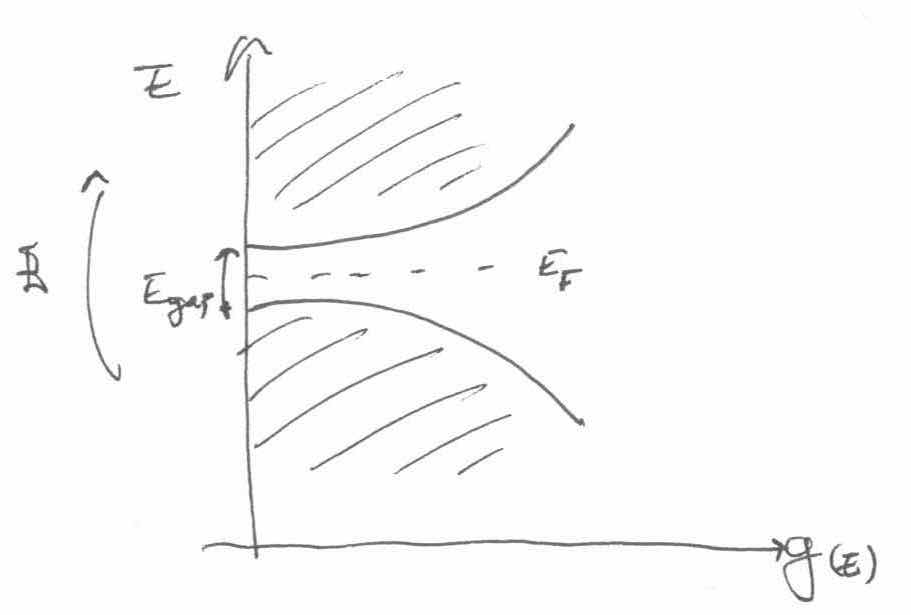
\includegraphics[height=4cm]{images/laser_80_2}
\end{figure}
\noindent
In tempi molto rapidi (pochi fs) gli elettroni eccitati in banda di conduzione e le lacune in banda di valenza termalizzano, cioè si raggiunge una condizione di quasi-equilibrio in cui la probabilità di occupazione degli elettroni in banda di conduzione e valenza è descritta da due distribuzioni di Fermi-Dirac:
\begin{equation*}
f_c(E) = \frac{1}{1+e^\frac{(E - E_{F_c})}{k_B T}}
\end{equation*}
\begin{equation*}
f_v(E) = \frac{1}{1+e^\frac{(E - E_{F_v})}{k_B T}}
\end{equation*}
dove $E_{F_c}$ ed $E_{F_v}$ sono detti quasi-livelli di Fermi in banda di conduzione e valenza. Sia $N$ la densità di portatori iniettati col pompaggio da banda di valenza a banda di conduzione. All'equilibrio termodinamico, se $N=0$, $E_{F_c} = E_{F_v} \equiv E_F$ energia di Fermi.
Se c'è pompaggio, $N\neq 0$, in situazione di quasi-equilibrio $E_{F_c} > E_{F_v}$. Significato fisico di $E_{F_c}$ ed $E_{F_v}$ (a $T\rightarrow0^+$):
\begin{figure}[H]
\centering
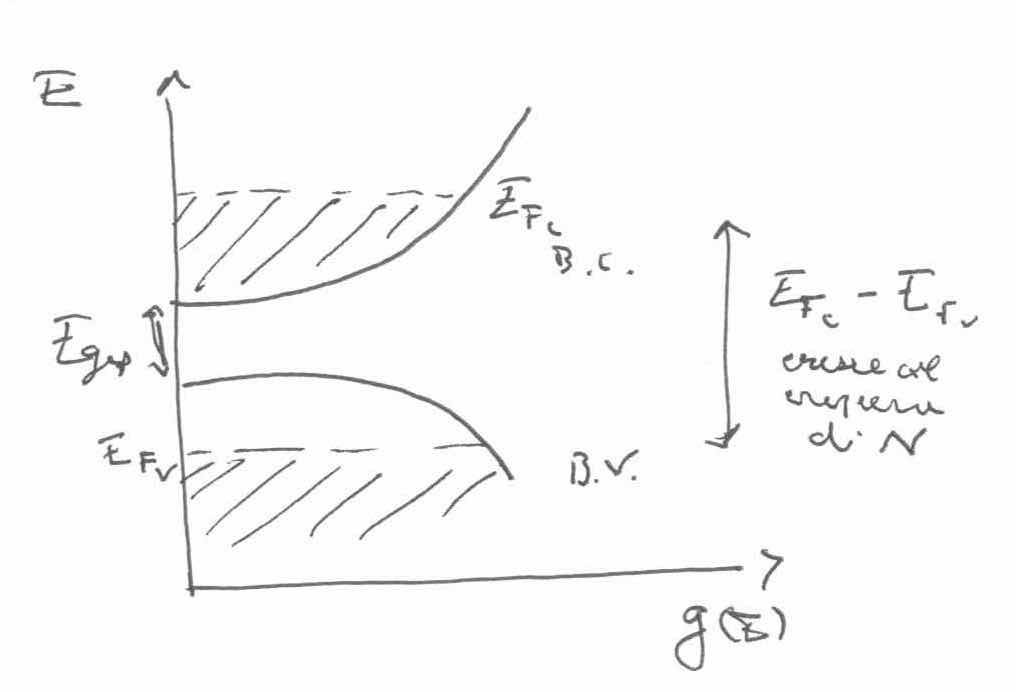
\includegraphics[height=4cm]{images/laser_80_3}
\end{figure}
\noindent
In tempi più lunghi, dell'ordine del tempo di ricombinazione elettrone-lacuna (decadimento radiativo o non radiativo), $\tau \sim 1ns$ nel GaAS, si raggiunge l'equilibrio termodinamico con un solo livello di Fermi $E_F$.

\section{Assorbimento ed emissione stimolata in un semiconduttore. Condizione di Bernard-Duraffourg}
Siano $\psi_v(\*r) = u_{\*k_v} |\*r| e^{i\*k_v \*r}$ e $\psi_c(\*r) = u_{\*k_c} |\*r| e^{i\*k_c \*r}$ che  funzioni di Bloch del cristallo corrispondente alle energie $E_2$, in banda di conduzione, ed $E_1$ in banda di valenza.
\begin{figure}[H]
\centering
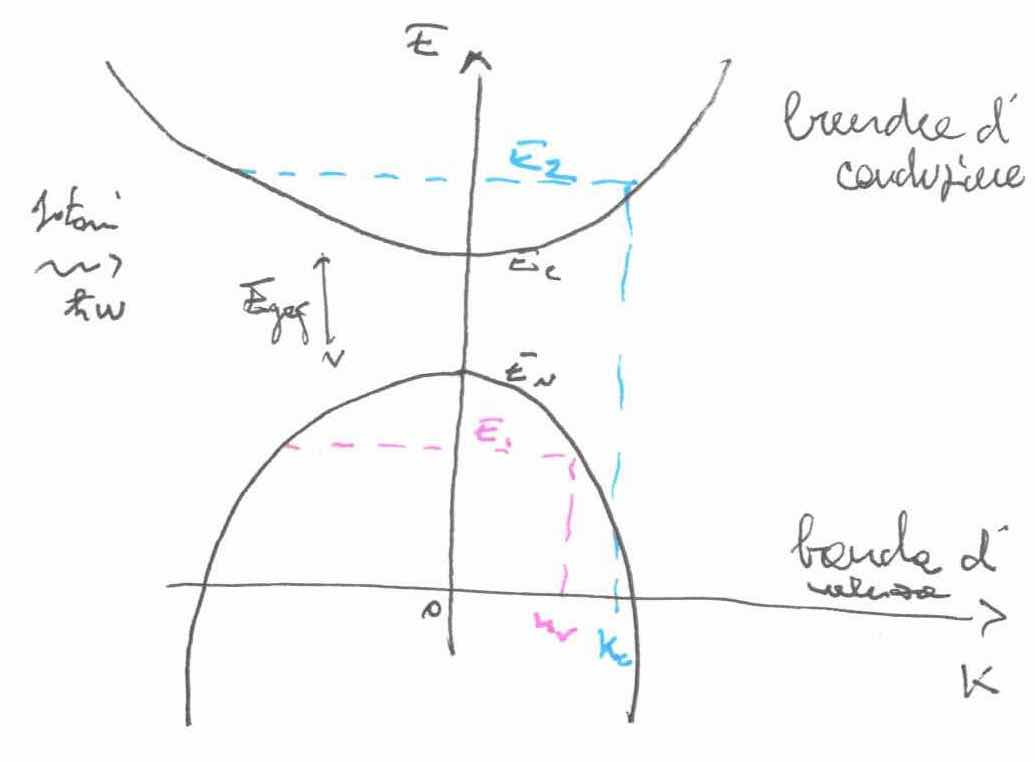
\includegraphics[height=4cm]{images/laser_80_4}
\end{figure}
\noindent
Sul cristallo incide un'onda e.m. monocromatica di frequenza $\w$ e campo elettrico:
\begin{equation*}
\*E(\*r,t) = \*E_0 e^{i\*k_{opt} \*r - i\w t}
\end{equation*}
Applicando la teoria di perturbazione ed assumendo una interazione di dipolo elettrico:
\begin{equation*}
\wh{H}_p = -\*\mu \*E = e\*r \*E
\end{equation*}
è noto che la probabilità nell'unità di tempo di indurre una transizione tra i due stati di Bloch $\psi_c$ e $\psi_v$ vale:
\begin{equation*}
W_{12} = W_{21} = \frac{\pi |\*P_{12}|^2}{2\hbar^2} \delta(\w - \w_0)
\end{equation*}
dove $\w_0 = \frac{E_2 - E_1}{\hbar}$ e $\left|\*P_{12}\right|^2 = \left| \int \psi_c*(\*r) e \*r \*E_0 e^{i\*k_{opt} \*r} \psi_v(\*r) d\*r \right|^2$
Si può dimostrare che $|\*P_{12}|^2 \neq 0$ se è soddisfatta la condizione:
\begin{equation*}
\hbar\*k_c = \hbar \hbar \*k_v + \hbar \*k_{opt}
\end{equation*}
che esprime la condizione di conservazione del momento.
Mentre la $\delta(\w - \w_0)$, cioè $W\neq 0$ se $\w = \w_0$, esprime la conservazione dell'energia. Siccome $|\*k_c|$, $\*k_v|$ sono, come ordine di grandezza, $\frac{\pi}{a}$ (a passo reticolare: tipicamente $a \lesssim 1nm$) mentre $|\*k_{opt}| = \frac{2\pi}{\l}$. Nel visibile ($\l \sim 500 nm$) $|\*k_{opt}| << |\*k_{v,c}|$.
Ciò comporta $\*k_c \sim \*k_v$ (trasmissione verticale nello spazio $\*k$).
Come corollario, segue che non posso usare semiconduttore a gap indiretta (es. Si o Ge) per fare amplificazione stimolata, e quindi un laser. Problema di integrazione tra laser e elettronica.
\begin{figure}[H]
\centering
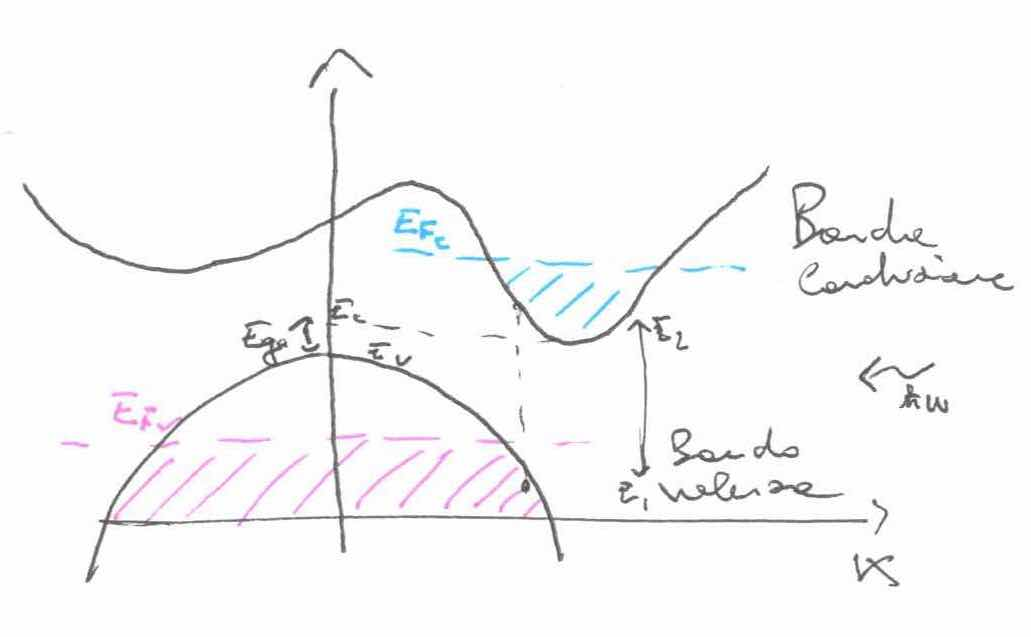
\includegraphics[height=4cm]{images/laser_80_5}
\end{figure}
\noindent
Se si deve avere transizione verticale per conservare il momento, in figura, non si può fare perché l'elettrone che decade dovrebbe andare dove ci sono già presenti due elettroni con spin opposto, quindi violando Pauli.\\
\\
Considero quindi un semiconduttore a gap diretta (es. GaAs, InP) e e chiediamo qual è la condizione tra $E_{F_c}$ ed $E_{F_v}$ per avere amplificazione di luce.
\begin{figure}[H]
\centering
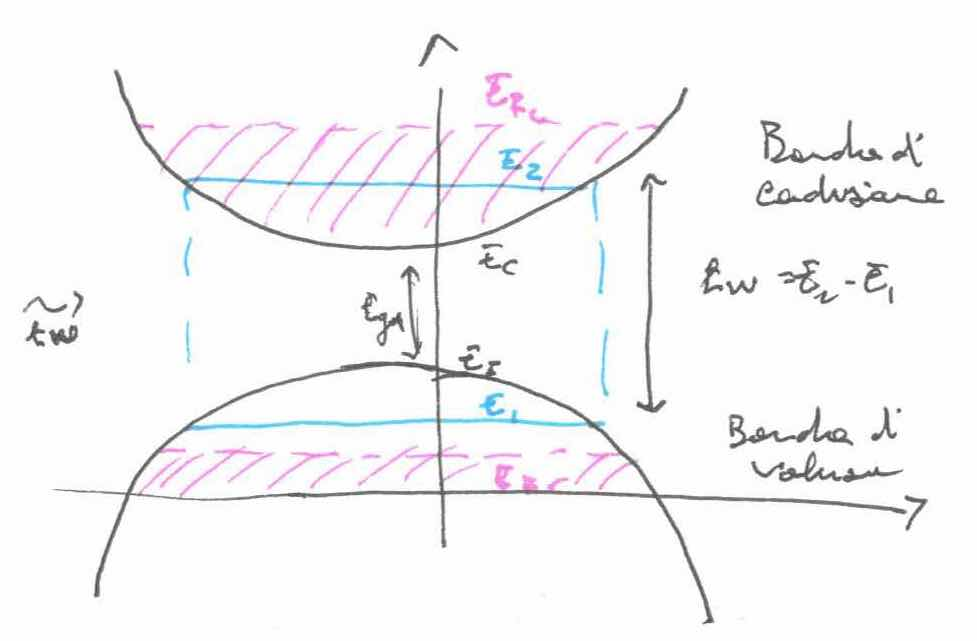
\includegraphics[height=4cm]{images/laser_80_6}
\end{figure}
\noindent
Notiamo che la probabilità che avvenga un processo si assorbimento è proporzionale al termine:
\begin{equation*}
\underbrace{f_v(E_1)}_\text{probabilità di avere elettroni in $E=E_1$} \cdot \underbrace{[1 - f_c(E_2)]}_\text{probabilità di non avere elettroni nel livello $E=E_1$}
\end{equation*}
Similmente, la probabilità che avvenga un processo di emissione stimolata è proporzionale a:
\begin{equation*}
\underbrace{f_c(E_2)}_\text{probabilità di avere elettroni in $E=E_2$ è occupato} \cdot \underbrace{[1 - f_v(E_1)]}_\text{probabilità di non avere elettroni nel livello $E=E_2$ è vuoto}
\end{equation*}
Affinché il semiconduttore amplifichi luce, deve aversi:
\begin{equation*}
f_c(E_2) \cdot [1 - f_v(E_1)] > f_v(E_1) \cdot [1 - f_c(E_2)]
\end{equation*}
cioè:
\begin{equation*}
f_c(E_2) > f_v(E_1)
\end{equation*}
\begin{equation*}
\frac{1}{1 + e^\frac{(E_2 - E_{F_c}}{k_BT}} > \frac{1}{1 + e^\frac{(E_1 - E_{F_v}}{k_BT}}
\end{equation*}
\begin{equation*}
E_2 - E_{F_c} < E_1 - E_{F_v}
\end{equation*}
cioè:
\begin{equation*}
E_2 - E_1 < E_{F_c} - E_{F_v}
\end{equation*}
Del resto, ovviamente $E_2 - E_1 > E_{gap}$ dove:
\begin{equation*}
E_g < E_2 - E_1 < E_{F_c} - E_{F_v}
\end{equation*}
condizione di amplificazione di Bernard-Duraffourg\\
Ciò significa che l'intervallo di frequenze $\w$ che vengono amplificate (banda di guadagno) in un semiconduttore pompato è:
\begin{equation*}
\frac{E_{gap}}{\hbar} < \w < \frac{E_{F_c} - E_{F_v}}{\hbar}
\end{equation*}
Interpretazione ovvia della condizione di Bernard-Douraffourg alla $T=0^+$:
\begin{figure}[H]
\centering
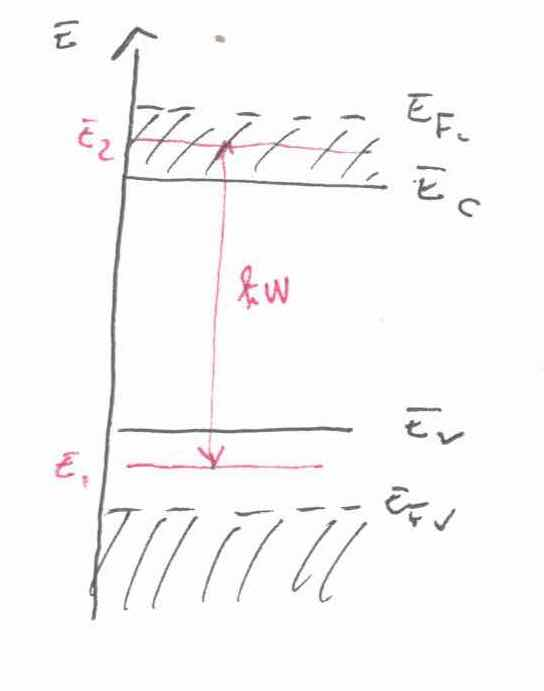
\includegraphics[height=4cm]{images/laser_80_7}
\end{figure}
\noindent
Si noti che per avere amplificazione, $N$ deve essere
\begin{equation*}
N \geq N_{th}
\end{equation*}
dove $N_{th}$ (densità di portatori iniettati a trasparenza) è il valore di $N$ per cui $E_{F_c} - E{F_v} = E_{gap}$.\\
\\
Tipico grafico del coefficiente di guadagno di un semiconduttore:
\begin{figure}[H]
\centering
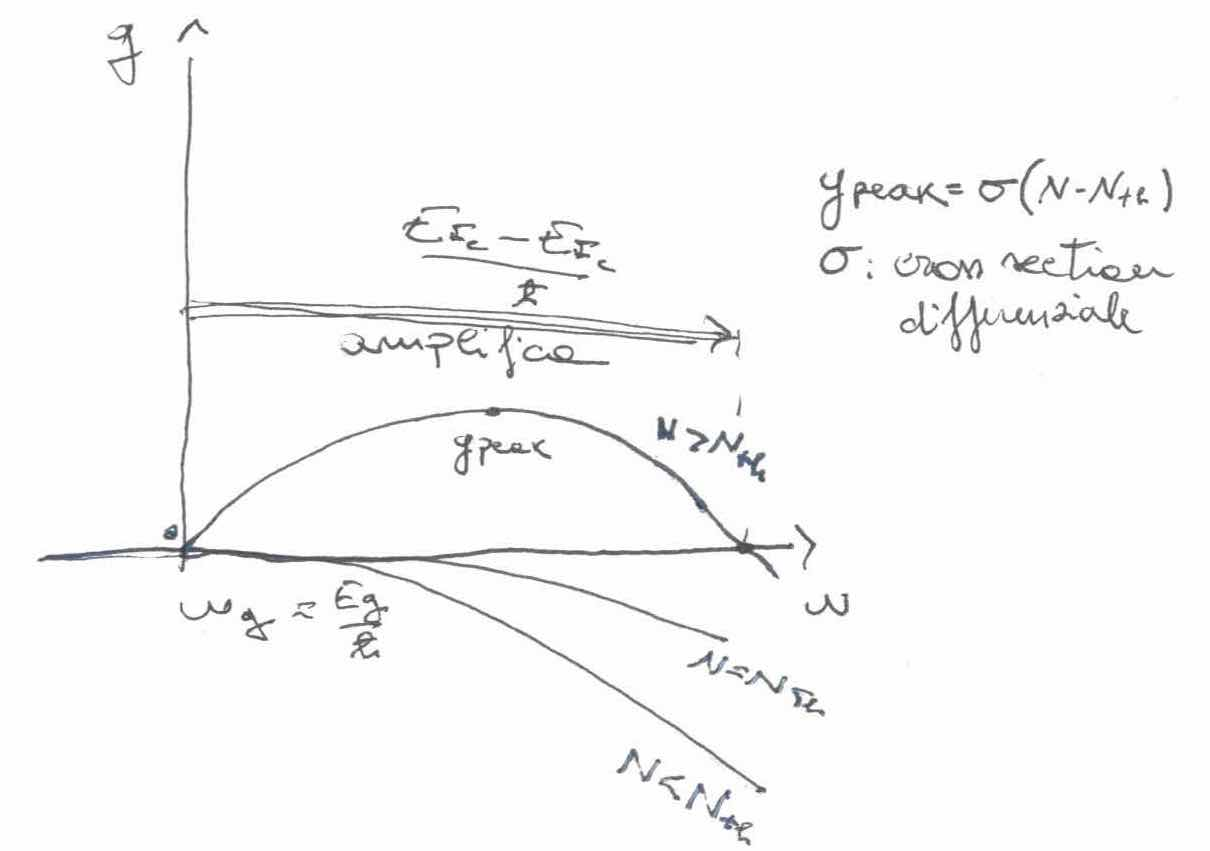
\includegraphics[height=4cm]{images/laser_80_8}
\end{figure}

\end{document}
